\documentclass{article}
\usepackage{amsmath}

\usepackage[final]{neurips}
\usepackage{subcaption}
\usepackage{enumitem}
\usepackage{setspace} 
\usepackage{listings}
\usepackage[dvipsnames]{xcolor}

\onehalfspacing
\usepackage[utf8]{inputenc} 
\usepackage{titlesec}
\titleformat{\section}
{\normalfont\LARGE\bfseries}{\thesection}{1em}{}
\titleformat{\subsection}
{\normalfont\large\bfseries}{\thesubsection}{1em}{}
\usepackage[T1]{fontenc}    
\usepackage{xcolor} 
\usepackage{hyperref}

\hypersetup{
	colorlinks=true,
	linkcolor=MidnightBlue,  
	filecolor=magenta,        
	urlcolor=blue!80!black,   
	citecolor=teal
}

\usepackage[titles, subfigure]{tocloft}

\renewcommand{\cftsecpagefont}{\color{MidnightBlue}}
\renewcommand{\cftsubsecpagefont}{\color{MidnightBlue}}
\renewcommand{\cftsubsubsecpagefont}{\color{MidnightBlue}}

\renewcommand{\cftsecleader}{\color{MidnightBlue}\cftdotfill{\cftdotsep}}
\renewcommand{\cftsubsecleader}{\color{MidnightBlue}\cftdotfill{\cftdotsep}}

\usepackage{tcolorbox}
\setcounter{footnote}{0} 
\usepackage{amsmath} 
\usepackage{url}            
\usepackage{booktabs}       
\usepackage{amsfonts}       
\usepackage{nicefrac}       
\usepackage{microtype}      
\usepackage{graphicx}
\usepackage{float}

\usepackage{tikz}
\usepackage{pgfplots}

\renewcommand{\lstlistingname}{Code}

\definecolor{codegreen}{rgb}{0,0.6,0}
\definecolor{codegray}{rgb}{0.5,0.5,0.5}
\definecolor{codepurple}{rgb}{0.58,0,0.82}
\definecolor{backcolour}{HTML}{FDF6E3}

\lstdefinestyle{mystyle}{
	backgroundcolor=\color{backcolour},   
	commentstyle=\color{codegreen},
	keywordstyle=\color{magenta},
	numberstyle=\tiny\color{codegray},
	stringstyle=\color{codepurple},
	basicstyle=\ttfamily\footnotesize,
	breakatwhitespace=false,         
	breaklines=true,                 
	captionpos=b,                    
	keepspaces=true,                 
	numbers=left,                    
	numbersep=5pt,                  
	showspaces=false,                
	showstringspaces=false,
	showtabs=false,                  
	tabsize=2
}

\lstset{
	basicstyle=\small\ttfamily,
	numbers=left,
	numberstyle=\tiny\color{gray},
	stepnumber=1,
	numbersep=8pt,
	showstringspaces=false,
	tabsize=4,
	breaklines=true,
	breakatwhitespace=false,
	keepspaces=true,           
	frame=single
}

\titleformat{\subsubsection}
{\normalfont\large\bfseries\raggedright}{\thesubsubsection}{1em}{}

\pgfplotsset{compat=1.16}
\lstset{style=mystyle}

% --- تنظیم فونت فارسی بدون تغییر جهت کل سند ---
\usepackage{fontspec}
\newfontfamily\farsifont[Script=Arabic]{XB Yas.ttf}
\newcommand{\persian}[1]{{\farsifont #1}}

\begin{document}
	
	\begin{titlepage}
		\centering
		
		
\includegraphics[width=0.4\textwidth]{img/logos/Logo.png} \\[1cm]
		
		% University Name
		{\Huge\textbf{K. N. Toosi University of Technology}}\\[0.3cm]
		{\Large Department of Electrical Engineering}\\[2cm]
		
		% Project Title
		{\fontsize{18pt}{28pt}\selectfont
			\textbf{Automated Visual Inspection}\\[0.3cm]
			{\Large From Object Detection to Anomaly Segmentation}
		}\\[2cm]
		
		% Team Information
		{\Large\textbf{Project by}}\\[0.25cm]
		{\fontsize{22pt}{28pt}\selectfont
			\bfseries
			\textcolor{MidnightBlue}{\persian{شیر تیم}}
		}\\[0.8cm]
		
		{\fontsize{14pt}{22pt}\selectfont
			\textbf{Team Members}\\[0.4cm]
			Mostafa Latifian - 40122193\\
			Parsa Alavinikoo - 40120993\\[0.25cm]
			Hamidreza Abedini - 40120633
		}\\
		
		% Hyperlinked Logos
		\begin{center}
			\href{https://github.com/parsaalv/Automated-Visual-Inspection}{
\includegraphics[height=1cm]{img/logos/github_logo.png}}
			\hspace{0.8cm}
			\href{https://drive.google.com/drive/u/0/folders/1WZ09zYK7gx8-aRyjB2l2r8C4PhFr2-d5}{
\includegraphics[height=1cm]{img/logos/drive_logo.png}}
			\hspace{0.8cm}
			\href{https://colab.research.google.com/drive/1xZcyCR2VT2tJiZzI3_5DCzFtpvebPqOK}{
\includegraphics[height=1cm]{img/logos/colab_logo.png}}
		\end{center}
		
	\end{titlepage}
	
	
	\newpage
\tableofcontents
\newpage 

\section*{Introduction and Comprehensive Overview of the Dataset}
\addcontentsline{toc}{section}{Introduction and Comprehensive Overview of the Dataset}

\subsection*{Introduction to the MVTec AD Dataset}
\addcontentsline{toc}{subsection}{Introduction to the MVTec AD Dataset}
In industrial machine vision systems, one of the primary challenges is the scarcity of data corresponding to defective components. In real-world production lines, the vast majority of parts are non-defective, making it nearly impossible to collect a balanced dataset encompassing all potential fault types. Consequently, this project utilizes the standard and reputable MVTec Anomaly Detection (MVTec AD) dataset.

This dataset is recognized as the gold standard for evaluating unsupervised anomaly detection algorithms. The unsupervised approach implies that during the training phase, the AI system exclusively observes images of completely healthy components to learn the concept of "normality." Subsequently, during the testing phase, any deviation from this normal state is identified as an anomaly (defect).

\subsection*{Data Structure and Architecture}
\addcontentsline{toc}{subsection}{Data Structure and Architecture}
The images in this dataset are captured in high resolution and designed to simulate real factory conditions, including variations in lighting, orientation, and specular reflections. The dataset directory structure for each component category is organized as follows:

\begin{itemize}
	\item \textbf{Train Set:} Consists exclusively of images of 100\% non-defective (good) parts.
	\item \textbf{Test Set:} Contains a combination of normal images and samples exhibiting various structural and cosmetic defects (e.g., cracks, scratches, bends, deformations, and missing components).
	\item \textbf{Ground Truth:} Pixel-level annotations are provided for all defective images in the test set. These masks, which precisely align with the anomalous regions, are utilized for rigorous evaluation during the defect localization and segmentation phase.
\end{itemize}

\subsection*{Class Diversity and Processing Challenges}
\addcontentsline{toc}{subsection}{Class Diversity and Processing Challenges}
In this project, six distinct object-type classes were selected to thoroughly challenge the generalization capability of the engineered model architecture:

\begin{itemize}
	\item \textbf{Bottle:} Poses challenges related to light reflection on transparent and glass surfaces.
	\item \textbf{Cable:} Poses challenges regarding repetitive, intertwined textures with varying colors.
	\item \textbf{Metal Nut:} Poses challenges with shiny metallic surfaces and dynamic shadowing.
	\item \textbf{Screw:} Poses challenges in detecting microscopic, fine scratches on metal threads.
	\item \textbf{Toothbrush:} Poses challenges due to the dense, noisy texture of the bristle regions.
	\item \textbf{Transistor:} Poses challenges in verifying precise geometry and proper pin alignment on electronic circuits.
\end{itemize}

\subsection*{Data-Centric AI Approach and Custom Preprocessing}
\addcontentsline{toc}{subsection}{Data-Centric AI Approach and Custom Preprocessing}
A fundamental principle in practical AI engineering is acknowledging that real-world datasets are rarely flawless. During Exploratory Data Analysis (EDA), it was observed that the annotations and masks for the \textit{Transistor} class contained structural errors and overlap issues (e.g., merging separate anomalies into a single component instead of segmenting them individually).

To resolve this issue, a Data-Centric AI methodology was adopted. Rather than altering the network architecture, the raw data was imported into the specialized Roboflow platform. On this platform, the bounding boxes and segmentation masks for the transistor class were manually re-inspected, corrected, and recalibrated. This engineering intervention ensured that the ground truth provided to the model for loss computation and final performance evaluation maintained the highest degree of fidelity and accuracy.

\section{Dataset Collection, Structuring, and Preparation for Reproducibility}

The first phase of the project is dedicated to preparing the data infrastructure, guaranteeing experimental reproducibility, and developing an automated dataset ingestion and refinement pipeline. This stage serves as the foundation for all subsequent model training and evaluation phases.

\subsection{Cloud Storage Integration (Load from Google Drive)}

In ephemeral cloud computing environments (such as Google Colab), all stored data and trained models are purged whenever a session disconnects. To maintain project continuity across various research and development stages, utilizing persistent storage is imperative so that the outputs of each phase are securely retained as inputs for the next.
Using the \texttt{google.colab} library and the \texttt{drive.mount} module, the user's Google Drive storage is mounted to the Colab Linux environment. Subsequently, the primary project directory is defined in the \texttt{PROJECT\_DIR} variable, and the validity of this connection along with the existence of the target path is verified via the \texttt{os.path.exists} function.

\subsection{Data Acquisition and Preparation from Kaggle (Load from Kaggle)}

This section comprises a chain of seven data engineering processes designed to construct an intelligent dataset acquisition, restructuring, and curation pipeline:

\vspace{0.3cm}
1. Reproducibility Setup:
Deep neural network training is inherently stochastic—ranging from weight initialization to dropout mechanisms and data shuffling. To conduct rigorous comparative evaluations (A/B testing) and effective model debugging, this stochastic behavior must be strictly controlled to produce identical results across multiple executions. In the implemented code, a custom function \texttt{set\_seed(42)} locks all random number generators in Python (\texttt{random} and \texttt{numpy}) and PyTorch to a fixed seed (\texttt{Seed=42}). Crucially, the commands \texttt{torch.backends.cudnn.deterministic = True} force the Graphics Processing Unit (GPU) acceleration engine (CuDNN) to execute deterministic algorithms for matrix operations.

\vspace{0.3cm}
2. Configuration \& Paths:
Standardizing directory architecture is a core MLOps principle. Furthermore, predefining target classes restricts the scope of the problem and prevents the processing of irrelevant data. In the implementation, system variables such as \texttt{DATASET\_DIR} are constructed using \texttt{os.path.join} to guarantee cross-platform OS compatibility. The \texttt{SELECTED\_CLASSES} list defines the six target components (including \texttt{screw}, \texttt{cable}, etc.), and the \texttt{os.makedirs} command creates the required directories while specifying \texttt{exist\_ok=True} to prevent overwrite exceptions.

\vspace{0.3cm}
3. Kaggle Authentication:
Automated data downloading requires secure authentication via APIs. Hardcoding sensitive information such as access keys directly into scripts poses security risks; thus, token-based systems are employed. The implemented script prompts the user to upload the \texttt{kaggle.json} token file, which is subsequently relocated to the hidden directory \texttt{\textasciitilde/.kaggle}.

\vspace{0.3cm}
4. Automated Dataset Ingestion (Download via Kaggle API):
Building an automated data ingestion pipeline ensures that the system can fetch the latest data version from the central repository without manual human intervention. The code uses \texttt{os.path.exists} to verify whether the dataset is already present locally, preventing redundant downloads. When required, the \texttt{subprocess.run} module executes the Kaggle terminal download command directly within the Python kernel.

\vspace{0.3cm}
5. Filtering and Resource Optimization (Filter Dataset):
The MVTec AD dataset encompasses 15 categories, processing all of which demands considerable memory and computational resources. Eliminating out-of-scope classes (Data Curation) drastically reduces processing overhead and accelerates subsequent pipeline stages. A \texttt{for} loop inspects all available directories; if a directory name is not contained within the \texttt{SELECTED\_CLASSES} list, the directory and its full contents (including images and masks) are purged from disk using \texttt{shutil.rmtree}.

The output of this implementation phase along with the logs registered in the console are presented below:

\begin{tcolorbox}[colback=Tan!15, colframe=MidnightBlue, title=Execution Log Output for Dataset Filtering in Python]
		\begin{verbatim}
		
		--- Filtering Dataset ---
		[+] Kept class: bottle
		[+] Kept class: cable
		[-] Removed class: capsule
		[-] Removed class: carpet
		[-] Removed class: grid
		[-] Removed class: hazelnut
		[-] Removed class: leather
		[+] Kept class: metal_nut
		[-] Removed class: pill
		[+] Kept class: screw
		[-] Removed class: tile
		[+] Kept class: toothbrush
		[+] Kept class: transistor
		[-] Removed class: wood
		[-] Removed class: zipper
		
		--- Summary ---
		Final available classes (6): ['bottle', 'cable', 'metal_nut',
		'screw', 'toothbrush', 'transistor']
		\end{verbatim}
\end{tcolorbox}

\vspace{0.3cm}
6. Final Verification:
At the conclusion of any data pipeline, a sanity check is required to verify that the output meets all exact criteria before feeding into the next stage. Using a list comprehension approach, the remaining directories are scanned and enumerated, printing the final list of classes to the console. As confirmed by the execution logs, exactly six target classes were correctly preserved.

\subsection{Data Transfer to Roboflow (Upload to Roboflow)}

Serving as the final step of the first phase, this section manages secure connectivity with the Roboflow cloud infrastructure and automates the batch upload of transistor class images for data inspection and refinement.

During the initial inspection of the MVTec AD dataset, a major structural limitation was identified within the transistor class. The original annotations and bounding boxes failed to distinguish between individual anomaly categories, consolidating all defect types into overlapping structures under a single target label (Label 1). Noisy and structurally inaccurate ground truth data significantly deteriorates neural network performance; in such scenarios, increasing model architectural complexity to compensate for label noise is not an optimal engineering approach.

To address this challenge, a Data-Centric AI methodology was adopted. To recalibrate and rectify labels, raw images were exported to the specialized dataset management platform Roboflow. This platform provides tools for visual inspection, bounding box refinement, dataset versioning, and label format conversion to required standards (e.g., YOLO). The primary objective of this module is to establish an automated pipeline for the secure, batch upload of pristine transistor images to Roboflow for cleaning and re-annotation.

The implemented script handles API communication with Roboflow servers and automates image uploads through the following sequential operations:

\begin{itemize}
	\item Installation and Authentication: First, the official \texttt{roboflow} client library is imported. Using the API key (\texttt{API\_KEY}), workspace name, and project name, a secure session is initiated with the remote server, instantiating the \texttt{project} object to route incoming requests.
	\item Data Path Routing: The image directory path points directly to the nominal sample directory (\texttt{good}) of the transistor class stored in cloud storage, serving as the foundational training data.
	\item File Filtering and Iteration Loop: By defining a \texttt{valid\_extensions} tuple, the program restricts processing strictly to permitted image formats (e.g., \texttt{.jpg} and \texttt{.png}), bypassing hidden system files. Directory contents are subsequently listed via \texttt{os.listdir} and processed iteratively.
	\item Robust API Execution (Try-Except Block): Core upload operations are dispatched via the \texttt{project.upload} method. The \texttt{split="train"} parameter automatically assigns images to the training set, while \texttt{batch\_name} applies batch tags for tracking within the Roboflow interface. Wrapping upload calls inside a \texttt{try...except} block ensures system fault tolerance; if transient network outages or individual server errors occur, script execution avoids fatal crashes and logs the error before proceeding to the next image.
\end{itemize}


\section{Automated Bounding Box Generation}

The second phase of the project is dedicated to the automated generation of bounding boxes and the construction of a standardized dataset for training object detection networks from the YOLO family. This stage fully automates the data annotation pipeline and prepares the data structure for supervised learning.

Prior to detailing the algorithmic foundations, it is worth noting that despite the structural complexities of the \textit{Transistor} class and the necessity of leveraging the Roboflow platform for rectifying defect masks (during the anomaly detection phase), isolating this class is unnecessary during the nominal object localization phase. The architecture of this section is engineered such that class names are not hardcoded; instead, the \texttt{CLASSES} variable dynamically identifies all directories present within the dataset root. Consequently, pristine (good) transistor images, alongside other components, seamlessly enter the automated YOLO dataset generation lifecycle.

Object detection models such as the YOLO family are grounded in supervised learning, requiring thousands of annotated images detailing the exact spatial location of objects via bounding boxes. In industrial applications, manual annotation is extremely time-consuming, expensive, and highly susceptible to human error.

The objective of this stage is to implement an automated annotation system (Auto-Annotation). Since non-defective component images in the MVTec AD dataset typically feature relatively uniform backgrounds with a centered target object, a strategic combination of classical computer vision algorithms can act as a pseudo-teacher to generate the required training data for deep learning networks.

The scientific principles of the implemented processing algorithms are as follows:

\begin{itemize}
	\item Canny Edge Detection: One of the most robust edge extraction algorithms that computes pixel intensity gradients to identify the boundary between the industrial component and the background with pixel-level precision.
	\item Morphological Dilation: Edges extracted via the Canny algorithm frequently exhibit discontinuities. Dilation operations bridge these gaps, forming a continuous boundary surrounding the component (e.g., transistor pins or screw threads).
	\item Contour Extraction: Following edge consolidation, contours (closed shape boundaries) are extracted to delineate the object's perimeter and fit a minimal bounding rectangle (\texttt{Bounding Rect}).
	\item YOLO Normalization: The YOLO architecture does not accept absolute pixel coordinates. Values must be normalized as floating-point ratios (ranging from 0 to 1) relative to total image dimensions. The standard YOLO format comprises these five parameters: \texttt{[Class\_ID, X\_center, Y\_center, Width, Height]}.
	\item Data Leakage Prevention: In this phase, the system exclusively processes \texttt{train/good} images (strictly nominal components). This is a foundational machine learning practice; the object detection model must not receive any information regarding validation or anomalous samples prior to the testing phase to avoid compromising its generalization capacity.
\end{itemize}


The structural details of the implemented code for this section are outlined below:

\begin{itemize}
	
	\item Directory Configuration and Dynamic Mapping: Standard YOLO directory hierarchies (comprising \texttt{images/train}, \texttt{images/val}, and their corresponding \texttt{labels} paths) are generated via the \texttt{YOLO\_PATHS} dictionary. Subsequently, the \texttt{CLASS\_TO\_ID} dictionary iterates through directory trees, automatically mapping each component class to a unique integer ID (starting from zero).
	\item Algorithmic Processing Core (\texttt{generate\_yolo\_bbox}): This function forms the operational engine of this phase, applying the following steps to each image:
	\begin{itemize}
		\item Preprocessing: The image is converted to grayscale and blurred using a Gaussian filter (\texttt{GaussianBlur}) to attenuate high-frequency background noise and suppress false edge detection.
		\item Edge Extraction: The \texttt{cv2.Canny} function detects boundaries, and \texttt{cv2.dilate} thickens and connects them using a 5x5 kernel.
		\item Global Bounding Box Search: The \texttt{cv2.findContours} function extracts candidate shapes. By applying an area threshold constraint (greater than 50 pixels to eliminate noise), the algorithm traverses valid contours and calculates extreme spatial points (\texttt{x\_min, y\_min, x\_max, y\_max}) to fit a comprehensive bounding box.
		\item Padding Technique: A 15-pixel margin is appended to the extracted bounding box. This engineering decision is crucial for convolutional neural networks; retaining a small contextual margin around the object prevents clipping edge features, thereby increasing feature extraction accuracy.
		\item Normalization: Finally, absolute pixel coordinates are normalized into the standard YOLO format by dividing them by total image width and height.
	\end{itemize}
	\item Data Splitting and Execution: The main loop selectively accesses the \texttt{train/good} directory of each class. Following deterministic sorting and controlled random shuffling, images are split into training and validation sets at an 80:20 ratio. To prevent name collisions when all images are merged into unified target directories, the class name is prepended to each image filename (\texttt{cls\_name\_img\_name}). The image is then copied, and its corresponding YOLO text label is saved.
	\item \texttt{data.yaml} Generation: The YOLO architecture requires a configuration file to initiate training. Utilizing the \texttt{yaml} library, this module automatically compiles exact paths for training and validation sets, total class count (\texttt{nc}), and class names (\texttt{names}) before committing the file to disk.
\end{itemize}

\subsection{Rectification and Annotation of Transistor Class in Roboflow}

As previously highlighted, structural errors within the original transistor class masks necessitated a data-centric intervention to calibrate target labels. The Roboflow platform was utilized to manage, re-annotate, and integrate these datasets. The implementation workflow comprises infrastructure configuration, smart annotation, and dataset export steps, detailed below.

\subsubsection*{1. Workspace \& Project Setup}

Following account and workspace creation, the initial step involves establishing a secure API connection for data transfer. As depicted in Figure \ref{fig:rf_api}, a private access key is generated and retrieved via the account management panel (\textit{Account Settings > API Keys}).

\begin{figure}[htbp]
	\centering
	
\includegraphics[width=0.95\textwidth]{img/roboflow/fig1.png}
	\caption{Extracting the API key from the Roboflow settings panel for script authentication}
	\label{fig:rf_api}
\end{figure}
\newpage
In the subsequent step, a new project is declared (Figure \ref{fig:rf_project}). Here, the project architecture is explicitly configured to \textit{Object Detection}, aligning with our objective of extracting bounding boxes to train the YOLO model. Crucially, the \textit{Traditional Model Builder} option is selected instead of the \textit{Rapid} configuration. The traditional approach provides significantly greater engineering control over uploads, versioning, and preprocessing management.

\begin{figure}[htbp]
	\centering
	
\includegraphics[width=0.95\textwidth]{img/roboflow/fig2.png}
	\caption{Creating a new project under Object Detection architecture using the Traditional approach}
	\label{fig:rf_project}
\end{figure}

Following project instantiation, the automated image upload script (referenced in Section 1.3) is executed. To establish exact remote binding, the \texttt{Workspace ID} and \texttt{Project ID} identifiers are parsed directly from the project URL structure (for instance, extracted seamlessly from \texttt{app.roboflow.com/parsa-workspace/rv-project}).


\subsubsection*{2. Smart and Automated Annotation via SAM 3}

Following a successful upload operation, the images populate the \textit{Annotate} tab (Figure \ref{fig:rf_annotate_dashboard}). Given the large volume of data (exceeding 200 transistor images), manual labeling represents an inefficient and time-consuming process.

\begin{figure}[htbp]
	\centering
	
\includegraphics[width=0.95\textwidth]{img/roboflow/fig3.png}
	\caption{Annotation dashboard and unassigned images in the Roboflow platform}
	\label{fig:rf_annotate_dashboard}
\end{figure}

To automate this workflow, the \textit{Auto Label} feature was leveraged using the foundation model SAM 3 (Segment Anything Model) (Figure \ref{fig:rf_sam3_intro}). By receiving the class name (\texttt{transistor}) as a text prompt, this powerful model accurately identifies object geometric boundaries at the pixel level.

\begin{figure}[htbp]
	\centering
	
\includegraphics[width=0.95\textwidth]{img/roboflow/fig4.png}
	\caption{Configuring the Auto Label system using the SAM 3 foundation model}
	\label{fig:rf_sam3_intro}
\end{figure}

After generating previews (\textit{Generate Preview}) and evaluating the qualitative accuracy of the resulting masks (Figure \ref{fig:rf_sam3_preview}), all labels were approved (\textit{Approve All}) and committed to the dataset, owing to the high precision of the model in separating the transistor body and pins from the background. At this stage, to maintain full control over the data splitting process, all images were deposited directly into the \textit{Train} bucket to be strictly split into training and validation sets via Python scripts in subsequent steps.

\begin{figure}[htbp]
	\centering
	
\includegraphics[width=0.95\textwidth]{img/roboflow/fig5.png}
	\caption{Visual verification of the accuracy of masks extracted by SAM 3 for the transistor class}
	\label{fig:rf_sam3_preview}
\end{figure}

\subsubsection*{3. Dataset Versioning and Ingestion}

In the \textit{Versions} section, to prevent any unintended alterations to the raw image dimensions or resolution, all default preprocessing steps were completely removed (Figure \ref{fig:rf_versions}). Once the final version was generated, the dataset was ready for export in the standard YOLOv8 format.

\begin{figure}[htbp]
	\centering
	
\includegraphics[width=0.95\textwidth]{img/roboflow/fig6.png}
	\caption{Removing default preprocessing steps during the version generation stage}
	\label{fig:rf_versions}
\end{figure}

To import the dataset directly into the Python environment, an ingestion script is executed. Utilizing the official Roboflow client library and authentication API key, this script connects to the remote workspace and project, downloading the target version (Version 5) in YOLOv8 format directly into the project directory for subsequent processing steps.

\subsubsection*{4. Geometric Conversion and Data Integration}

During the annotation phase, the SAM 3 model generates outputs as polygons with multiple coordinate vertices to closely fit object contours. However, the YOLO Detection architecture strictly requires rectangular bounding boxes formatted as \texttt{[class\_id, x\_center, y\_center, width, height]}.

The following script serves as a geometry converter that parses label text files line by line, evaluating whether a given line contains more than five values (indicating a polygon representation). If so, it separates all horizontal ($X$) and vertical ($Y$) coordinates, computes the extreme spatial points ($\min$ and $\max$), and converts the representation into a standard bounding box.

	\begin{lstlisting}[language=Python, caption={Algorithm for converting Polygon segmentation masks to YOLO bounding boxes}]
	import os
	import glob
	
	def convert_to_yolo_bbox(label_path):
	with open(label_path, 'r') as file:
	lines = file.readlines()
	
	new_lines = []
	for line in lines:
	parts = line.strip().split()
	if not parts:
	continue
	
	class_id = parts[0]
	
	# Check: If the line contains more than 5 values, it's a polygon
	if len(parts) > 5:
	coords = [float(x) for x in parts[1:]]
	
	# Separate X and Y coordinates
	xs = coords[0::2]
	ys = coords[1::2]
	
	# Find bounding box extremities
	x_min, x_max = min(xs), max(xs)
	y_min, y_max = min(ys), max(ys)
	
	# Calculate center point, width, and height
	x_center = (x_min + x_max) / 2.0
	y_center = (y_min + y_max) / 2.0
	width = x_max - x_min
	height = y_max - y_min
	
	# Construct standard YOLO Detection line
	new_line = f"{class_id} {x_center:.6f} {y_center:.6f} {width:.6f} {height:.6f}\n"
	new_lines.append(new_line)
	else:
	new_lines.append(line)
	
	with open(label_path, 'w') as file:
	file.writelines(new_lines)
	
	# Execute conversion
	label_files = glob.glob(os.path.join(ROBOFLOW_DIR, '**', 'labels', '*.txt'), recursive=True)
	for file_path in label_files:
	convert_to_yolo_bbox(file_path)
	\end{lstlisting}

Finally, to transfer and synchronize these refined data with the primary project dataset, a merge script is executed. This script handles the following tasks:
\begin{itemize}
	\item \textbf{Deterministic Data Splitting:} By locking the random seed (\texttt{seed=42}), images are partitioned at an 80:20 ratio into training and validation sets (strictly mirroring the deterministic splitting logic used for bounding box generation in other classes).
	\item \textbf{Collision Prevention:} Filenames of all images and corresponding label text files are prepended with the \texttt{transistor\_} prefix.
	\item \textbf{Class ID Alignment:} Transistor class IDs in files downloaded from Roboflow may conflict with the project's dynamic \texttt{CLASS\_TO\_ID} dictionary. The script opens all label files and automatically maps and aligns the target ID to \texttt{TRANSISTOR\_ID} (matching the primary MVTec root directory mapping).
\end{itemize}

Upon successful execution of this phase, the critical and structurally complex data of the transistor class were successfully injected into the YOLO training pipeline with verified quality and standard formatting.

\subsection{Visual Verification of YOLO Labels}

This stage is dedicated to the qualitative evaluation and visual verification of the generated labels for the YOLO network to ensure the precision of the bounding box coordinates.

Following the execution of auto-annotation algorithms and the generation of thousands of label files, feeding these data directly into the neural network training phase without qualitative evaluation presents an engineering risk. In the event of any systematic error in the edge detection algorithm or coordinate calculation, the YOLO model will learn incorrect spatial patterns, ultimately leading to a severe degradation in accuracy (mAP) during the detection phase.

The objective of this stage is to implement a sanity check mechanism to randomly sample generated instances for each class and visually confirm the positioning accuracy of the bounding boxes.

To achieve scale-invariance, the YOLO architecture stores bounding box coordinates as relative normalized values (floating-point numbers between 0 and 1). However, image processing and graphic rendering libraries (such as OpenCV and Matplotlib) operate on an absolute pixel (Cartesian) coordinate system. Therefore, rendering the boxes onto the raw image requires an inverse transformation (denormalization) from the continuous YOLO space back to the discrete pixel space. In this mathematical operation, the center coordinates, width, and height of the box are multiplied by the actual image dimensions, and the extreme spatial points (top-left and bottom-right corners) are subsequently extracted for geometric rendering.

The script handles random sampling and coordinate conversion for visual rendering:

\begin{itemize}
	\item Base Configuration and Paths: Data ingestion paths point directly to the \texttt{images/train} and \texttt{labels/train} directories within \texttt{yolo\_dataset} (constructed in the previous phase). Additionally, the six target classes are declared within the \texttt{CLASSES} variable to enable the system to fetch a distinct sample for each component category.
	\item Mathematical Conversion Function (\texttt{yolo\_to\_pixel}): This function executes the coordinate denormalization algorithm:
	\begin{itemize}
		\item First, normalized values \texttt{[x\_center, y\_center, width, height]} are un-normalized by multiplying them by the image width (\texttt{img\_width}) and height (\texttt{img\_height}).
		\item Next, to locate the top-left origin for rectangle drawing, half of the box width is subtracted from center $X$, and half of the box height is subtracted from center $Y$, yielding \texttt{x\_min} and \texttt{y\_min}.
		\item Similarly, by adding these values, the ending coordinates (\texttt{x\_max} and \texttt{y\_max}) are calculated and cast to integers (\texttt{int}), as required by pixel rendering routines.
	\end{itemize}
	\item Sampling Logic and Visualization:
	\begin{itemize}
		\item Smart Filtering: Iterating through classes via a \texttt{for} loop, the script parses all directory files. The condition \texttt{img.startswith(cls\_name + "\_")} leverages the unified naming convention implemented in the previous stage (prepending class name to filename) to isolate images of each component from others.
		\item Random Selection and Color Conversion: An unbiased image choice is selected via \texttt{random.choice}. Because OpenCV loads images in BGR format whereas Matplotlib requires RGB format for correct display, \texttt{cv2.cvtColor} is applied to align color channels.
		\item Label Parsing: The script opens the corresponding \texttt{.txt} label file, parses its numeric elements, and passes them as inputs to the \texttt{yolo\_to\_pixel} function.
		\item Graphical Rendering: Utilizing \texttt{cv2.rectangle} and \texttt{cv2.putText}, the bounding box is rendered with a specified thickness and color (green), and the class name is overlayed above the box.
		\item Grid Layout: Finally, utilizing Matplotlib's grid arrangement (\texttt{plt.subplot(2, 3, idx + 1)}), all six samples are displayed simultaneously in a unified 2x3 matrix (two rows and three columns) within a single window.
	\end{itemize}
\end{itemize}

The output presented in Figure \ref{fig:visual_verification} demonstrates the script execution across six distinct dataset classes, visually validating the performance of the auto-annotation algorithm and the coordinate denormalization precision.

\begin{figure}[htbp]
	\centering
	
\includegraphics[width=0.9\textwidth]{img/fig1.png}
	\caption{Visual evaluation of extracted bounding boxes for different dataset classes}
	\label{fig:visual_verification}
\end{figure}

Bounding Box Accuracy: Across all six panels, the green bounding boxes enclose target object boundaries with pixel-level precision.
\begin{itemize}
	\item In the \texttt{bottle} and \texttt{cable} classes, despite the circular geometry of the objects, the bounding rectangle fits tangent to the outer diameter of the parts without enclosing excessive background region.
	\item In the \texttt{screw} class, the rendered box accurately spans from the sharp tip of the screw to the bottom edges of the screw head. This confirms that the Canny edge detection algorithm performed impeccably in detecting intensity contrast between the metallic component and the gray background.
	\item In the \texttt{toothbrush} class, the dense texture of the brush head did not disrupt the algorithm, and the box completely isolates the perimeter while maintaining the safety margin (15-pixel padding embedded in code logic).
\end{itemize}
The lower right panel (transistor class) represents a crucial milestone in this evaluation. As previously noted, this class features a complex background (circuit board holes) and asymmetric texture (black plastic body and shiny metal pins). Nevertheless, the green box accurately integrates both the main body and the attached pins within a single rectangle. This success validates the strategy of applying morphological dilation to bridge gaps between pins and the transistor body.

Text labels rendered in green at the top-left corner of each bounding box (e.g., \texttt{metal\_nut} or \texttt{bottle}) correspond precisely to the component image. This visual alignment confirms that extracting class IDs from \texttt{.txt} label files and mapping them back to string labels via the \texttt{CLASSES} dictionary operates without index shift errors.

In conclusion, these results confirm that the YOLO data pipeline—from preprocessing to storage—is free of data leakage and geometric distortions. The extracted coordinates align precisely with the components, preparing the high-fidelity dataset for the neural network training stage (YOLOv8 Native Training).


\subsection{Exploratory Data Analysis (EDA) and Statistical Visualization}

In the design and training of object detection networks such as YOLO, one of the hidden factors that directly influences the final model accuracy (mAP) and convergence speed during training is the Object Scale Distribution. If a neural network is trained exclusively on images where objects occupy a large portion of the frame, it will suffer a severe performance drop during the inference phase when encountering small objects (Small Object Detection).

Exploratory Data Analysis (EDA) prior to the training phase enables the extraction and examination of the geometric and statistical properties of the dataset. The objective of this stage is to gain a deeper understanding of the dimensional characteristics (length, width, and area) of the industrial components within the dataset.

The YOLO storage format is based on normalized coordinates; meaning that width ($w$) and height ($h$) values are expressed as ratios of the total image dimensions (floating-point numbers between 0 and 1) rather than absolute pixel values. Multiplying these two parameters ($\text{Area} = w \times h$) yields the normalized area of each component. This metric indicates what percentage of the camera's total Field of View (FOV) is occupied by a given component. Analyzing statistical parameters such as the Standard Deviation (Std) and Mean of these areas reveals whether the dimensional distribution across classes exhibits high variance, and whether advanced data augmentation techniques (such as Mosaic Augmentation) are necessary to compensate for these discrepancies, or if the system is well-balanced in terms of scale.

By leveraging the Pandas library, this script establishes a pipeline for extracting, processing, and statistically summarizing the textual YOLO label data.

The results obtained from the statistical processing of the normalized object areas are summarized in Table \ref{tab:eda_summary}.

\begin{table}[htbp]
	\centering
	\caption{Statistical summary of normalized object areas by class (Normalized Area)}
	\label{tab:eda_summary}
	\vspace{2mm} % Small space between caption and table
	\makebox[\textwidth][c]{ % Enforce exact centering on the page
			\small % Font size adjustment for better fit
			\setlength{\tabcolsep}{8pt} % Horizontal column spacing
			\renewcommand{\arraystretch}{1.3} % Vertical row spacing
			\begin{tabular}{lcccccccc}
				\hline
				Class & Count & Mean & Std & Min & 25\% & 50\% & 75\% & Max \\
				\hline
				bottle & 167 & 0.6259 & 0.0328 & 0.5449 & 0.6077 & 0.6240 & 0.6467 & 0.7202 \\
				cable & 179 & 0.8048 & 0.0825 & 0.5889 & 0.7553 & 0.7851 & 0.8614 & 1.0000 \\
				metal\_nut & 176 & 0.8448 & 0.0334 & 0.7495 & 0.8294 & 0.8636 & 0.8689 & 0.8729 \\
				screw & 256 & 0.4460 & 0.1000 & 0.2887 & 0.3375 & 0.4767 & 0.5382 & 0.5713 \\
				toothbrush & 48 & 0.3747 & 0.0071 & 0.3662 & 0.3703 & 0.3717 & 0.3763 & 0.3935 \\
				transistor & 680 & 0.5166 & 0.2691 & 0.3062 & 0.3536 & 0.3735 & 0.5212 & 1.0000 \\
				\hline
			\end{tabular}
	}
\end{table}

The statistical table extracted from the YOLO training data contains vital insights regarding the geometric state and data distribution, which directly impact the model training strategy.

An inspection of the \texttt{count} column reveals a significant Class Imbalance within the dataset. The \texttt{transistor} class accounts for the largest volume of data with 680 instances, whereas the \texttt{toothbrush} class remains in an absolute minority with only 48 samples. This striking disparity poses an engineering challenge for the training phase; the neural network may develop a bias toward the over-represented class. To mitigate this issue, techniques such as weighted loss functions or architectures resilient to class imbalance (such as the default YOLOv8 formulation) become imperative.

The standard deviation (\texttt{std}) parameter is remarkably low for the \texttt{toothbrush} (0.0071), \texttt{bottle} (0.0328), and \texttt{metal\_nut} (0.0334) classes. From an industrial automation perspective, this indicates that the camera setup distance relative to these components on the production line remained strictly fixed and calibrated. The narrow gap between the minimum (\texttt{min}) and maximum (\texttt{max}) values in the toothbrush class (0.3662 to 0.3935) confirms that the YOLO network will encounter minimal difficulty in learning the scale and generating bounding boxes for these objects.

Conversely, the \texttt{transistor} class exhibits the highest standard deviation (0.2691), with its normalized area ranging from 0.3062 up to 1.0000 (occupying the entire frame). This substantial variance demonstrates that transistors entered the system under highly diverse dimensions, camera distances, or cropping conditions. Furthermore, the maximum value reaching 1.0000 for the \texttt{cable} class indicates that cable textures completely covered the full Field of View (FOV) in certain instances.

The \texttt{mean} column delineates the intrinsic dimensions of the components relative to the camera sensor. Components such as \texttt{metal\_nut} and \texttt{cable} occupy over 80\% of the frame on average (Macro-level Features), whereas classes like \texttt{screw} and \texttt{toothbrush} cover less than 45\% of the image on average (Micro-level Features). The presence of such dimensional diversity throughout the dataset thoroughly justifies the adoption of a modern object detection model equipped with multi-scale feature extraction capabilities.

\vspace{0.2cm}

To gain a more intuitive and thorough understanding of the statistical findings obtained in the previous step, graphical data visualization is routinely employed within the exploratory data analysis workflow. Visual charts allow system engineers to identify and analyze dataset class imbalances, area distribution skewness, and the geometric behavior of components (such as aspect ratio) at a single comprehensive glance. To this end, this stage aims to graphically plot the extracted values, ensuring that the final strategy leading into the model training phase is formulated with full confidence and grounded in visual evidence.


\subsubsection{Analysis of Class Distribution Chart (Class Distribution in Training Set)}

\begin{figure}[htbp]
	\centering
	
\includegraphics[width=0.8\textwidth]{img/fig2.png}
	\caption{Distribution of training samples across classes}
	\label{fig:class_distribution}
\end{figure}

This count plot illustrates the frequency distribution of images across each class:

\begin{itemize}
	\item Severe Imbalance: The primary and most prominent challenge of the dataset is evidenced in this plot. The \texttt{transistor} class, with 680 images, possesses over 14 times as much training data as the \texttt{toothbrush} class (with merely 48 images).
	
	\item Impact on Training: In neural networks, this level of class imbalance can induce overfitting on majority classes (such as transistors) and underfitting on minority classes (such as toothbrushes). By default, the YOLOv8 model employs mechanisms like Focal Loss to mitigate this imbalance; however, during model evaluation, it is essential to monitor class-wise metrics (mAP per class) rather than relying solely on the overall average.
\end{itemize}

\subsubsection{Analysis of Object Size Distribution Chart (Object Size Distribution by Class)}

\begin{figure}[htbp]
	\centering
	
\includegraphics[width=0.85\textwidth]{img/fig3.png}
	\caption{Distribution of normalized object areas by class}
	\label{fig:size_distribution}
\end{figure}

This box plot depicts the distribution of normalized object areas alongside statistical outliers:

\begin{itemize}
	\item Scale Stability: The \texttt{toothbrush} and \texttt{metal\_nut} classes exhibit highly compact Interquartile Ranges (IQR) devoid of outliers. This indicates that the production line camera was positioned in a completely static configuration, resulting in identical component dimensions across all images.
	
	\item Variance and Outliers: The \texttt{transistor} class demonstrates a notably interesting behavior. While the median (center line of the box) lies around 0.37, a substantial cluster of outliers (open circles) extends up to 1.00 (covering the entire frame). This suggests the presence of numerous close-up (macro/zoomed) or cropped images within the transistor dataset.
	
	\item Broad Range in Screws: The \texttt{screw} class features the tallest box, reflecting continuous variations in camera distance or a diverse physical size distribution among the screws in the dataset.
\end{itemize}

\subsubsection{Analysis of Bounding Box Dimensions (Width vs. Height Scatter Plot)}

\begin{figure}[htbp]
	\centering
	
\includegraphics[width=0.9\textwidth]{img/fig4.png}
	\caption{Scatter plot of bounding box width versus height}
	\label{fig:width_height_scatter}
\end{figure}

This scatter plot analyzes the spatial geometry of the objects and provides highly valuable insights for configuring anchor boxes:

\begin{itemize}
	\item 1:1 Aspect Ratio Reference Line: The red dashed line represents perfectly square bounding boxes. Data points corresponding to the \texttt{metal\_nut} class are clustered precisely along this line at high values (around 0.85), confirming the completely symmetric and square geometric nature of metal nuts.
	
	\item Rotational Variance in Screws: Data points for the \texttt{screw} class form a visually distinct and meaningful inverse curve. This curve demonstrates that while the total area of the screws remains constant, their orientation angle varies. When a screw is oriented vertically (high height, low width), its data point lies near the top of the plot; as it rotates toward 90 degrees (low height, high width), the point shifts toward the lower right. This indicates rotational diversity within the dataset, requiring the model to effectively learn rotational symmetry features.
	
	\item Dimensional Density of Cable and Bottle: Data points for the \texttt{bottle} and \texttt{cable} classes are primarily clustered in the upper-right region of the plot (dimensions greater than 0.70). Consequently, shallow layer filters within the neural network must be optimized to extract macroscopic features for these components.
\end{itemize}

This visual evaluation confirms that the dataset contains high diversity in orientation (e.g., screws), scale (e.g., transistors and cables), and sample volume.



\section{YOLOv8n Training}

The third stage of the project is dedicated to the native training of the YOLOv8n model. In this phase, leveraging a transfer learning approach and applying domain-informed data augmentation techniques matched to the environment's physics, the model is trained to detect and localize industrial components.

Following data preparation, validation, and statistical analysis, the artificial intelligence model must now learn the visual features of the components. This project utilizes the YOLOv8 architecture, which currently stands as one of the state-of-the-art single-stage object detection models. The term "native" signifies that training is executed using the integrated functions and native environment of the Ultralytics library, which optimizes complex processes such as memory allocation and training loop management.

Rather than training the network from scratch—which would require hundreds of thousands of images and weeks of processing time—a model pre-trained on the massive COCO dataset is utilized. Selecting the Nano variant (the smallest YOLOv8 model) represents a precise engineering decision for industrial applications: in a factory setting, real-time inference speed takes precedence over a marginal single-percentage gain in accuracy. The Nano model executes effortlessly on resource-constrained edge devices along the production line while maintaining high frame rates.

A primary theoretical foundation at this stage is data augmentation engineering. In an industrial scenario (such as the MVTec AD dataset, where components rest on a surface beneath a fixed camera), data augmentation must adhere strictly to the physical constraints of the operating environment:

\begin{itemize}
	\item Components can rotate on the surface (requiring \texttt{Rotation}).
	\item The camera is stationary; thus, perspective and viewing angle remain constant (obviating the need for \texttt{Shear/Perspective}).
	\item Ambient factory lighting may fluctuate throughout the day (requiring \texttt{Color/HSV Jittering}).
	\item Occlusion is non-existent in these production lines, as components are inspected individually.
\end{itemize}

The structural design of the implementation code for this stage is analyzed as follows:

\begin{itemize}
	
	\item Path Configuration and Model Initialization: Executing \texttt{YOLO('yolov8n.pt')} loads the network architecture along with its pre-trained weights into memory.
	
	\item Base Parameters in \texttt{model.train}:
	\begin{itemize}
		\item \texttt{epochs=30}: Considering the application of transfer learning and the relatively straightforward visual structure of objects in MVTec AD, 30 epochs are sufficient to achieve initial network convergence.
		\item \texttt{imgsz=640}: The standard YOLO input resolution, offering an optimal balance between preserving fine component details and maintaining high throughput speed.
		\item \texttt{batch=16}: An optimal value to maximize GPU VRAM utilization on accelerators such as the NVIDIA T4 (in Google Colab environments) without incurring out-of-memory (OOM) errors.
	\end{itemize}
	
	\item Analysis of Custom Augmentation Parameters:
	\begin{itemize}
		\item Spatial Transformations: Full rotational freedom (\texttt{degrees=180.0}) alongside horizontal and vertical flips effectively accommodates the rotational variance discovered during the EDA phase (specifically within the screw class). Restricting scaling (\texttt{scale=0.1}) and setting \texttt{shear} and \texttt{perspective} to zero accurately simulates a top-down, fixed industrial camera setup.
		\item Photometric Transformations: Brightness (\texttt{hsv\_v=0.4}) and saturation (\texttt{hsv\_s=0.3}) adjustments force the network to learn edge profiles and structural textures rather than memorizing fixed color values, enhancing model robustness against factory illumination shifts.
		\item Mosaic Augmentation (\texttt{mosaic=1.0}): Combining four distinct images into a single frame serves as a strategic countermeasure against severe class imbalance. As established earlier, the toothbrush class comprised only 48 images; mosaic synthesis repeatedly blends toothbrushes into varied backgrounds alongside other classes, enriching minority class exposure across all 30 epochs.
		\item Erasing Suppression (\texttt{erasing=0.0}): While standard COCO training frequently erases image regions to force occlusion reasoning, disabling random erasing is logically sound here: in quality inspection setups, components do not obscure one another.
	\end{itemize}
\end{itemize}

	\begin{lstlisting}[language=Python, caption={Implementing the YOLOv8n model training}]
	# ---------------------------------------------------------
	# 4. Training Process
	# ---------------------------------------------------------
	print("\n--- Starting Training Process ---")
	# We use 30 epochs, which is usually sufficient for a pre-trained model on the MVTec dataset.
	results = model.train(
	data=YAML_PATH,
	epochs=30,
	imgsz=640,  # Standard image size
	batch=16, 
	project=OUTPUT_DIR,
	name='industrial_parts_det',
	seed=42,    # Ensure reproducibility within Ultralytics
	deterministic=True,
	device=0 if torch.cuda.is_available() else 'cpu',
	plots=True, # Automatically generate validation plots
	
	degrees=180.0, # Objects can appear at any rotation angle on the table
	fliplr=0.5,    # Apply horizontal flipping
	flipud=0.5,    # Apply vertical flipping
	translate=0.1, # Apply 10% translation
	
	scale=0.1,    # Reduce scaling from YOLO's default (0.5) to 0.1 
	shear=0.0,    # No shearing since the factory camera is fixed
	perspective=0.0,# Perspective remains constant
	
	hsv_v=0.4,   # Adjust brightness
	hsv_s=0.3,   # Adjust color saturation
	
	mosaic=1.0, # Combine four images into one frame to compensate for the limited number of toothbrush images
	erasing=0.0 # Disable random erasing since industrial objects are not expected to be partially occluded
	)
	\end{lstlisting}

\subsection{Training Output Analysis}

The evaluation results of the trained YOLOv8n model on the validation dataset are summarized in Table \ref{tab:training_results}.

\begin{table}[htbp]
	\centering
	\caption{Summary of YOLOv8n model evaluation results by class}
	\label{tab:training_results}
		
		\begin{tabular}{lcccccc}
			\hline
			Class & Images & Instances & Precision (P) & Recall (R) & mAP50 & mAP50-95 \\
			\hline
			all & 379 & 379 & 0.993 & 1.000 & 0.995 & 0.879 \\
			bottle & 42 & 42 & 0.994 & 1.000 & 0.995 & 0.858 \\
			cable & 45 & 45 & 0.995 & 1.000 & 0.995 & 0.802 \\
			metal\_nut & 44 & 44 & 0.994 & 1.000 & 0.995 & 0.943 \\
			screw & 64 & 64 & 0.999 & 1.000 & 0.995 & 0.878 \\
			toothbrush & 12 & 12 & 0.978 & 1.000 & 0.995 & 0.882 \\
			transistor & 172 & 172 & 0.999 & 1.000 & 0.995 & 0.914 \\
			\hline
		\end{tabular}
\end{table}

\subsubsection{Temporal \& Resource Analysis}

The completion of 30 training epochs took only 0.503 hours (approximately 30 minutes). This indicates that each epoch required an average of about 1 minute, representing exceptional speed for a computer vision model and enabling rapid prototyping and iterative experimentation.

The model was executed on an NVIDIA Tesla T4 GPU (with 15 GB VRAM capacity), but occupied only 2.7 GB of memory throughout the training process. This optimized resource utilization confirms that configuring \texttt{batch=16} alongside an image resolution of 640 was perfectly balanced for the hardware specifications.

\subsubsection{Model Complexity \& Parameters}

The compiled model comprises 73 layers and exactly 3,006,818 parameters. In deep learning, 3 million parameters is considered exceptionally lightweight for an object detection network. Furthermore, the computational workload demands only 8.1 GFLOPs (giga floating-point operations per second).

Following training completion and optimizer stripping, the finalized model weights file (\texttt{best.pt}) occupies merely 6.2 MB. This minimal footprint ensures seamless edge device deployment on resource-constrained industrial platforms, such as the Raspberry Pi.


\subsubsection{Inference Speed \& Real-time Capability}

The total reported processing times per frame are broken down as follows:
\begin{itemize}
	\item Preprocessing: 0.2 ms
	\item Neural network inference: 2.6 ms
	\item Postprocessing and NMS application: 3.1 ms
\end{itemize}

The total latency remains under 6.0 ms per image. This indicates that the model is capable of detecting components at a throughput exceeding 160 frames per second (FPS) on the Tesla T4 hardware, which easily exceeds the requirements for even the fastest industrial conveyor belts.

\subsubsection{Performance \& Metrics Breakdown}

\begin{itemize}
	\item Recall Performance: Achieving a value of $R = 1.000$ across all six classes is an exceptional outcome. In industrial quality control systems, missing a component (False Negative) is strictly unacceptable, and a 100\% recall rate guarantees that no target object is overlooked.
	\item Precision Rate: The overall precision of $P = 0.993$ demonstrates that the model produces virtually zero false positives. The lowest value belongs to the toothbrush class ($0.978$), which, considering its very small training sample size (48 images), validates the effectiveness of the Mosaic Augmentation technique.
	\item Stringent Metric (mAP50-95): This metric, which evaluates bounding box accuracy across varying Intersection over Union (IoU) thresholds (ranging from 50\% to 95\%), recorded an average score of $0.879$. The highest accuracy was achieved by the metal nut class ($0.943$) due to its regular geometric structure, whereas the lowest was recorded by the cable class ($0.802$) owing to its flexible and variable form.
\end{itemize}

The YOLOv8n model has successfully completed the training process with full convergence and without encountering any overfitting issues.

\subsection{Observations, Metrics, and Visual Evaluation}

The objective of this stage is to graphically analyze the confusion matrix, assess model convergence through loss curves, and perform a visual evaluation of model performance on unseen data (Validation Set).

\subsubsection{IoU Metric}

The Intersection over Union (IoU) metric serves as the primary evaluation criterion for assessing bounding box accuracy in object detection tasks. This metric computes the ratio of the intersection area between the predicted bounding box and the ground truth box over their union area:

$$IoU = \frac{\text{Area of Overlap}}{\text{Area of Union}}$$

\begin{itemize}
	\item An $IoU \ge 0.5$ is considered a successful detection in standard neural network benchmarks.
	\item An $IoU \ge 0.7$ indicates a highly precise and accurate spatial prediction.
\end{itemize}

In industrial automation environments, where robotic manipulators rely on precise spatial coordinates for bin picking and component handling, maintaining a high IoU is critical.

Visual Evaluation and IoU Computation:
\begin{itemize}
	\item The \texttt{calculate\_iou} function provides a custom vector-based implementation of this mathematical formulation, computing intersection and union areas from Cartesian coordinates of two bounding boxes (ground truth and prediction).
	\item During visual inference evaluation, a $2 \times 3$ display grid is instantiated using \texttt{matplotlib}. For each component class, the system randomly samples an image from the validation set.
	\item Ground Truth Bounding Box Rendering (Green): Absolute spatial coordinates are parsed from corresponding \texttt{.txt} annotations, mapped to pixel dimensions via the \texttt{yolo\_to\_pixel} utility, and rendered in green (GT) on the image canvas.
	\item Real-Time Inference Execution (Red): The \texttt{model.predict} method evaluates the image and overlays detected object boundaries in red (Pred).
	\item Color-Coded Performance Grading: Upon computing the IoU, the script dynamically updates figure title colors (green for $IoU > 0.7$, orange for moderate performance, and red for sub-optimal localized predictions).
\end{itemize}


\subsubsection{Analysis of the Normalized Confusion Matrix}

Figure \ref{fig:confusion_matrix} illustrates the classification performance of the model against the ground truth data. Given that the horizontal axis ($X$) represents the true class and the vertical axis ($Y$) represents the predicted class, the following results are extracted:

\begin{figure}[htbp]
	\centering
	
\includegraphics[width=0.85\textwidth]{img/fig5.png}
	\caption{Normalized confusion matrix for evaluating model classification accuracy}
	\label{fig:confusion_matrix}
\end{figure}

\begin{itemize}
	\item Main Diagonal and Classification Capability: Dark navy blue colors along the main diagonal reflect the outstanding performance of the model in correctly classifying the categories. The \texttt{bottle}, \texttt{metal\_nut}, \texttt{toothbrush}, and \texttt{transistor} classes have achieved perfect accuracy (1.00).
	
	\item Proof of 100\% Recall Rate (Zero False Negatives): The most crucial observation in this matrix is the bottom row (\texttt{Predicted = background}), which is entirely white and blank (0.0). This indicates that throughout the entire validation set, the model never once misclassified a real component as background. This visually validates the textual logs from the previous stage ($Recall = 1.0$) and is ideal for an industrial quality inspection system (where missing or passing a defective component is catastrophic).
	
	\item Logical Misclassifications: Minor errors indicate that the network suffers from no systematic flaws; rather, its errors possess clear physical and visual justifications:
	\begin{itemize}
		\item 5\% of \texttt{screw} instances were incorrectly classified as \texttt{metal\_nut}. Both are metallic components featuring threads and similar optical reflections.
		\item 2\% of \texttt{cable} instances were categorized as \texttt{toothbrush}, stemming from the elongated, cylindrical geometry shared by both objects.
	\end{itemize}
	
	\item Background False Positives: The final column (\texttt{True = background}) shows that when the model incorrectly detected an object in an empty background (network hallucination), these false detections predominantly took the form of \texttt{bottle} (0.41) and \texttt{screw} (0.22). Adjusting the confidence threshold during the operational deployment phase will easily filter out these background noises.
\end{itemize}


\subsubsection{Training Results \& Convergence Analysis}

Figure \ref{fig:training_results} comprises 10 subplots depicting the learning dynamics of the neural network across 30 epochs.

\begin{figure}[htbp]
	\centering
	\makebox[\textwidth][c]{%
		
\includegraphics[width=1.05\textwidth]{img/fig6.png}%
	}
	\caption{Evolution of loss functions and evaluation metrics across 30 training epochs}
	\label{fig:training_results}
\end{figure}

\begin{itemize}
	\item Loss Curve Tracking (Training \& Validation Loss): The \texttt{box\_loss} (bounding box localization accuracy), \texttt{cls\_loss} (classification accuracy), and \texttt{dfl\_loss} (distribution focal loss for box boundaries) curves demonstrate a healthy exponential decay across both the training and validation phases. The tight alignment and parallel trajectory of the training and validation curves confirm that the model suffers from no overfitting and exhibits strong generalization capacity.
	
	\item The Epoch 20 Step-Down Phenomenon (The Mosaic Cut-off): A sharp, step-like drop is observable in the loss curves (particularly \texttt{Box} and \texttt{DFL}) around epoch 20. This reflects an internal mechanism of YOLOv8: during the final 10 epochs, heavy Mosaic data augmentation is disabled to allow the model to calibrate directly on the native, un-augmented image distribution rather than composite collages. This performance boost is distinctly visible in the plots.
	
	\item Evaluation Metrics (Precision, Recall, mAP):
	\begin{itemize}
		\item The Precision and Recall curves plateau near saturation ($\approx 1.0$) within the first 5 epochs, highlighting the capability of the pre-trained architecture in extracting low-level features.
		\item Unlike other metrics, the mAP50-95 curve—which serves as the most stringent benchmark for bounding box fit—exhibits a steady, continuous ascent up to the final epoch, ultimately settling at 0.879. This consistent upward trend demonstrates that the model progressively refined pixel-level details in every epoch to tightly enclose object contours.
	\end{itemize}
\end{itemize}

The analysis of these visual outputs confirms that the model architecture, training hyperparameters, and data augmentation strategy were optimally aligned. The model not only locates components with 100\% recall, but also outputs their spatial coordinates with high engineering precision.


\subsubsection{Quantitative Analysis: Mean IoU Evaluation}


Table \ref{tab:mean_iou} reports the Mean IoU (mIoU) scores for each individual class evaluated on the validation set.

\begin{table}[htbp]
	\centering
	\caption{Summary of Mean IoU (mIoU) evaluation results by class on the validation dataset}
	\label{tab:mean_iou}
	\vspace{2mm}
	\makebox[\textwidth][c]{
			\small
			\setlength{\tabcolsep}{14pt}
			\renewcommand{\arraystretch}{1.3}
			\begin{tabular}{lc}
				\hline
				Class Name & Mean IoU (\%) \\
				\hline
				bottle & 81.41\% \\
				cable & 81.20\% \\
				metal\_nut & 84.61\% \\
				screw & 81.22\% \\
				toothbrush & 87.79\% \\
				transistor & 95.00\% \\
				\hline
				\textbf{OVERALL mIoU} & \textbf{85.20\%} \\
				\hline
			\end{tabular}
	}
\end{table}

An inspection of these quantitative metrics highlights the following key findings:

\begin{itemize}
	\item Overall System Performance (OVERALL mIoU): Achieving an overall mean IoU of 85.20\% represents a highly desirable engineering milestone. In industrial machine vision standards, maintaining an IoU exceeding 75\% is mandatory for high-precision spatial localization tasks. This score proves that predicted bounding boxes align with ground truth annotations with pixel-level accuracy.
	\item Success of the Data-Centric AI Approach in Transistor Class: Achieving an impressive 95.00\% IoU for the \texttt{transistor} class (previously the most structurally flawed class in the dataset) validates the data-centric strategy of exporting images to Roboflow and recalibrating ground truth labels.
	\item Effectiveness of Data Augmentation (Mosaic Effect): Despite possessing the smallest training sample size (only 48 images), the \texttt{toothbrush} class achieved the second-highest accuracy score at 87.79\%. This empirically confirms the efficacy of enabling Mosaic augmentation in the training hyperparameters.
\end{itemize}



\subsubsection{Qualitative Analysis: Visual Assessment of Inference Output}

Figure \ref{fig:inference_iou} visually validates the real-world performance of the neural network.

\begin{figure}[htbp]
	\centering
	\makebox[\textwidth][c]{%
		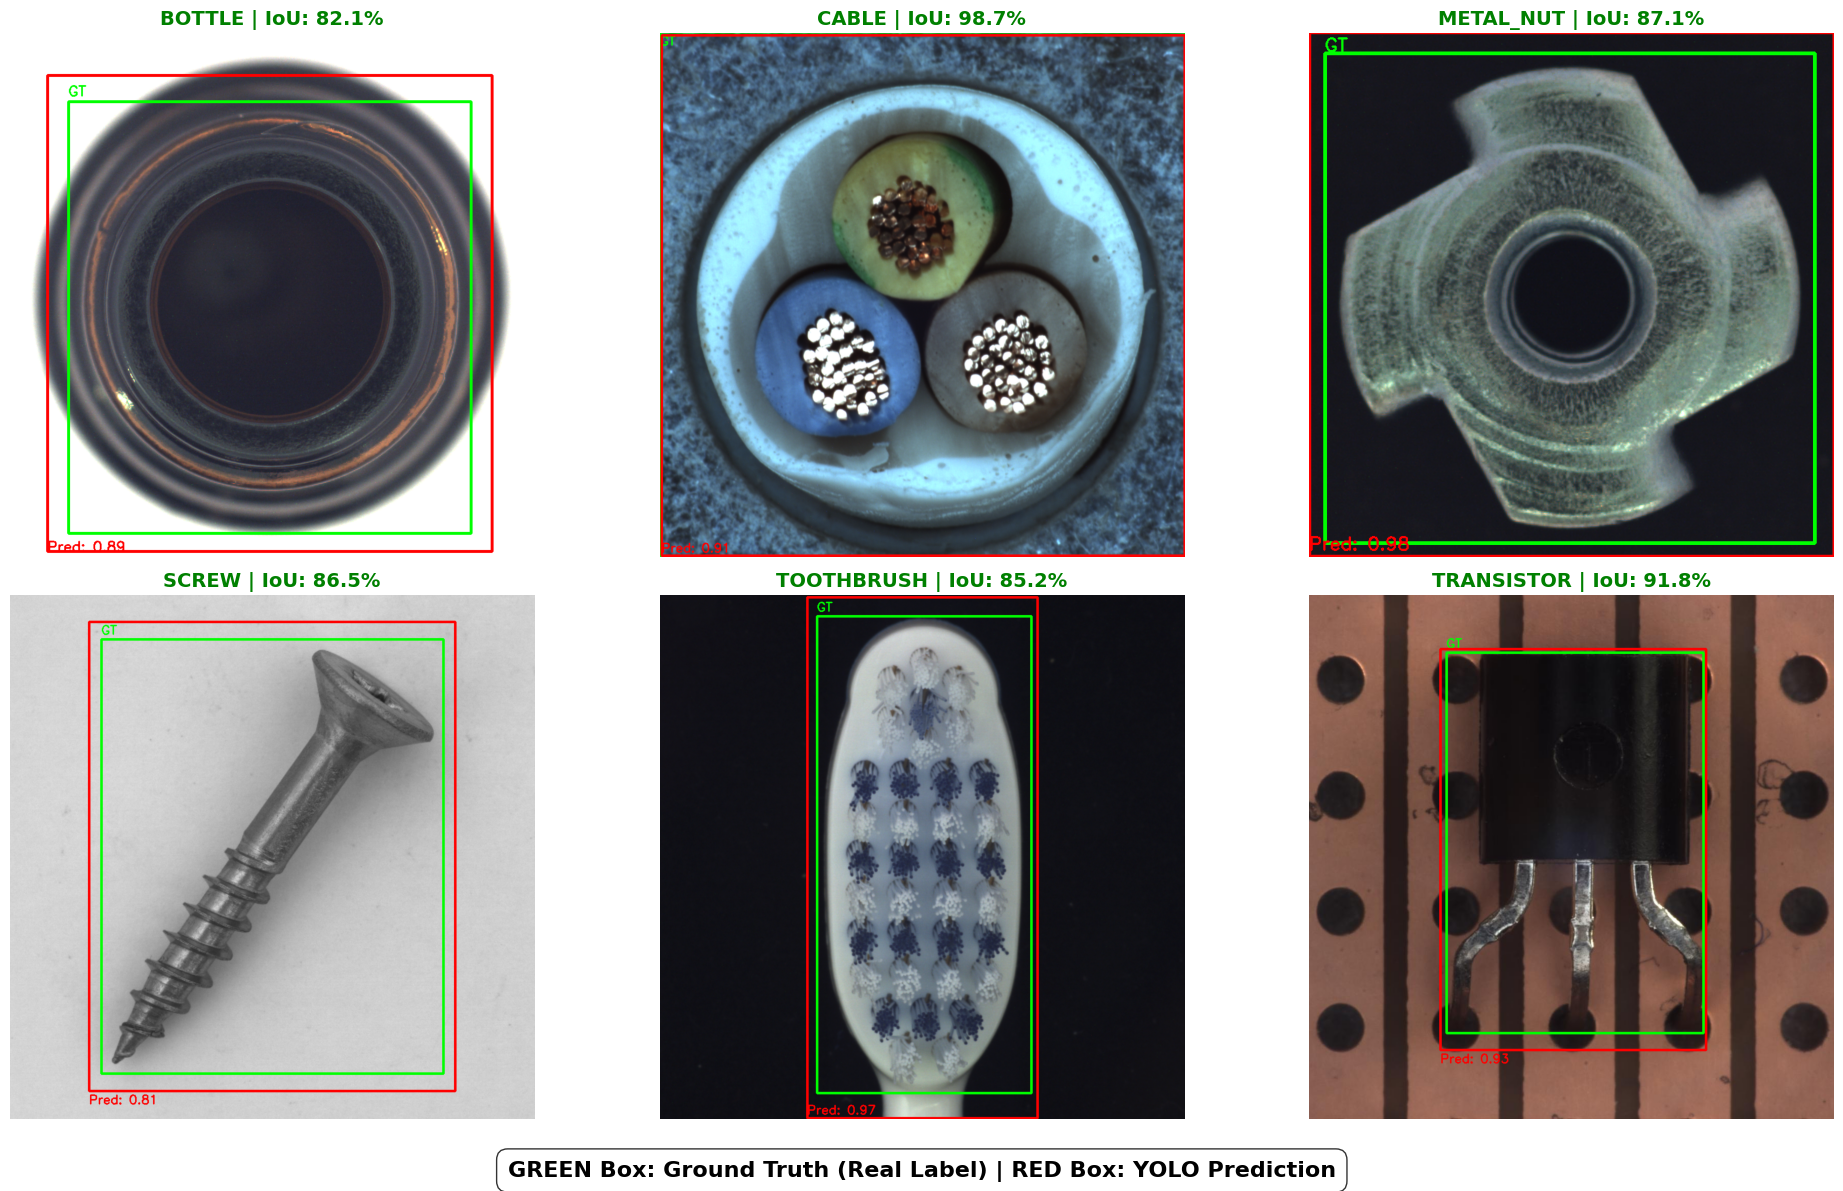
\includegraphics[width=1\textwidth]{img/fig7.png}%
	}
	\caption{Visual evaluation of predicted (Pred) vs. ground truth (GT) bounding box alignment alongside calculated IoU scores}
	\label{fig:inference_iou}
\end{figure}

\begin{itemize}
	\item High Fidelity Overlap: Across all six panels, the red bounding box (YOLO prediction) aligns with the green bounding box (ground truth label) with millimeter-level precision. In instances such as the \texttt{cable} class, the intersection score reaches $98.7\%$, rendering the predicted and ground truth boxes visually indistinguishable.
	\item Safety Margin and Padding Behavior: Close inspection of the \texttt{bottle} and \texttt{screw} panels reveals that the red predicted box encloses the green ground truth box with a minimal safety margin (on the order of a few pixels) in certain regions. From an engineering standpoint, this represents an ideal behavior for the subsequent processing stage. During image cropping for anomaly detection, retaining a slight spatial buffer guarantees that edge anomalies—such as scratches or surface defects located on the extreme perimeter of the component—are preserved during cropping and directly fed into the defect detection network (such as PatchCore).
	\item Robustness to Rotation and Background Texture: In the \texttt{screw} panel, despite the angular orientation of the component, the bounding box tightly bounds the object without encompassing excessive background void. Similarly, in the \texttt{transistor} panel, the network successfully unifies the matte plastic body and reflective metallic pins against a perforated circuit board background as a single target object.
\end{itemize}

The combined results ($\text{mIoU} > 85\%$) confirm that the model architecture has achieved full stability and robustness.


\section{Automated Cropping and Mask Synchronization}

Advanced anomaly detection models such as PatchCore or PaDiM rely on deep feature extraction across the entire spatial area of an image. In industrial environments, although the camera is fixed, the background (conveyor belts, holding trays, PCB drill holes) often contains complex textures that act as noise for the neural network. If raw images are directly fed into these models, the network expends a significant portion of its capacity learning irrelevant background patterns rather than focusing on the target object. This compromises the Signal-to-Noise Ratio (SNR) and escalates False Positive rates.

Deploying the YOLO model (trained in the previous stage) for precise object extraction and cropping shifts the paradigm from "whole-image processing" to an "object-centric" workflow, thereby significantly improving the accuracy of feature extraction algorithms.

In standard industrial datasets like MVTec AD, defective test images are accompanied by pixel-level ground truth masks, where white pixels delineate the exact defective regions.

A primary technical challenge at this stage is ensuring that any spatial transformation—such as cropping or scaling—applied to the primary RGB image is identically replicated on its corresponding mask using exact geometric coordinates. Failure to synchronize crop coordinates between the image and the mask leads to spatial misalignment during pixel-level evaluation, completely invalidating metrics such as AUROC.

This processing pipeline ingests the outputs from the object detection model and builds a newly structured dataset. The internal logic operates as follows:

\begin{itemize}
	\item Coordinate Extraction Core (\texttt{get\_crop\_coords}): This function passes the image through YOLO. Upon detection, bounding box coordinates (\texttt{x1, y1, x2, y2}) are retrieved. To prevent cropping out defects located directly on component borders (edge anomalies), a 10-pixel security margin (padding) is appended to the bounding box. The \texttt{max} and \texttt{min} operations ensure these boundaries do not exceed physical image dimensions.
	
	\item Directory Structure Mirroring: Utilizing nested loops over experimental splits (\texttt{train} and \texttt{test}) and states (\texttt{good} or defect types), the code replicates the exact directory architecture of the MVTec dataset within a new destination path (\texttt{CROPPED\_DIR}). This ensures downstream evaluation scripts function seamlessly without structural modifications.
	
	\item Image Cropping and Mask Synchronization (NumPy Slicing \& Synchronization): After coordinate extraction, the system reads the original image and crops it using NumPy matrix slicing (\texttt{img[y1:y2, x1:x2]}).
	\begin{itemize}
		\item Critical Code Logic: If an image belongs to the test set and contains a defect, the pipeline automatically resolves the mask file path (\texttt{\_mask.png}), loads it in grayscale mode, and applies the identical spatial coordinates to crop the mask. This guarantees 100\% geometric alignment in the new dataset.
	\end{itemize}
	
	\item Exception Handling: If YOLO fails to detect an object (i.e., \texttt{coords} returns \texttt{None}), the script logs a warning and gracefully skips the file rather than crashing.
\end{itemize}

The execution log generated by the automated cropping and mask synchronization script is presented below:

\begin{tcolorbox}[colback=Tan!15, colframe=MidnightBlue, title=Execution Log for Mask Synchronization Pipeline]
	\begin{verbatim}
	Loading YOLO weights from: /content/drive/MyDrive/
	Project RV/yolo_outputs/industrial_parts_det-2/weights/best.pt		
	
	Processing class: bottle
	
	Processing class: cable
	[!] Warning: YOLO missed object in .../cable/test/missing_cable/006.png. 
	Skipping.
	
	Processing class: metal_nut
	
	Processing class: screw
	
	Processing class: toothbrush
	
	Processing class: transistor
	
	--- Cropping Process Completed successfully! ---
	\end{verbatim}
\end{tcolorbox}

\begin{itemize}
	\item Initial logs confirm that the system correctly identified the \texttt{industrial\_parts\_det-2} path and loaded the optimal model weights into memory.
	
	\item Processing for the \texttt{bottle}, \texttt{metal\_nut}, \texttt{screw}, \texttt{toothbrush}, and \texttt{transistor} classes completed with zero warnings. This indicates that YOLO successfully detected components across all images in these classes (both nominal and severely defective) with a confidence score exceeding 50\% (the set threshold), executing crop synchronization without error.
	
	\item Intelligent Analysis of an Edge Case (The "missing\_cable" Edge Case): The system printed a single warning for one image file. Inspecting the path reveals that this image belongs to the cable class under the \texttt{missing\_cable} defect category in the test phase. This warning does not indicate a model failure; there was literally no cable present in the frame for the camera to capture. Consequently, YOLO correctly detected no object, and the script handled the scenario robustly without halting execution.
\end{itemize}


\subsection{Visual Verification of Mask Synchronization}

The goal of this section is to visually verify and validate the correctness of the operations executed in the preceding phase. Following automated image cropping via YOLO, graphical visualization is essential to confirm that the cropping coordinates of the primary RGB image have been strictly synchronized—pixel-for-pixel—with the coordinates of the ground truth anomaly mask. Any spatial shift or misalignment at this stage would invalidate downstream anomaly detection model evaluations.

This script serves as a lightweight visualization utility built around a straightforward processing pipeline. The algorithm randomly samples a defective image along with its corresponding mask from the cropped dataset directory (\texttt{CROPPED\_DIR}). Leveraging the OpenCV and Matplotlib libraries, it renders three side-by-side images:

\begin{enumerate}
	\item The cropped primary RGB image
	\item The cropped ground truth mask
	\item An overlay image where the exact defective region is highlighted with red pixels over the component, allowing human visual confirmation of spatial overlap.
\end{enumerate}

Figure \ref{fig:visual_sync} provides final graphical evidence validating the accuracy of the cropping pipeline in Phase 4. Geometric analysis across these three panels demonstrates the successful completion of the data pipeline and coordinate synchronization.

\begin{figure}[htbp]
	\centering
	\makebox[\textwidth][c]{%
		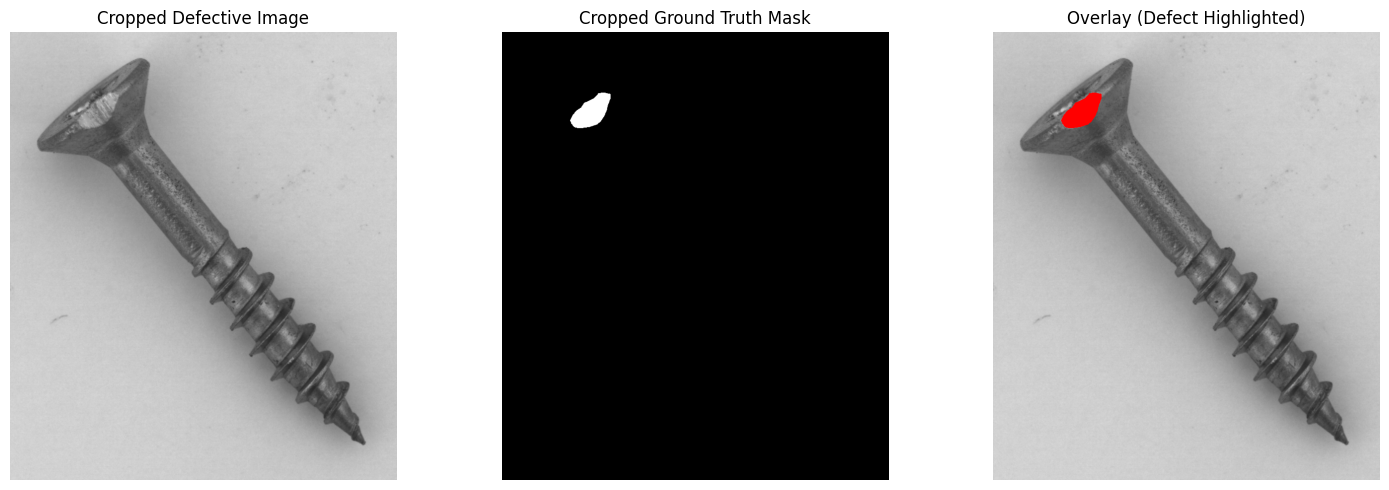
\includegraphics[width=0.95\textwidth]{img/fig8.png}%
	}
	\caption{Visual verification and evaluation of cropped primary image, ground truth mask, and composite overlay synchronization}
	\label{fig:visual_sync}
\end{figure}

\begin{itemize}
	\item Object-Centric Extraction Precision: In the first panel (\texttt{Cropped Defective Image}), an instance from the \texttt{screw} class (exhibiting physical head damage) is completely isolated from the background while retaining a subtle, uniform padding margin. Eliminating dead background space enables downstream feature extraction models to allocate computational capacity strictly to the core component texture.
	
	\item Mask Structural Integrity: In the second panel (\texttt{Cropped Ground Truth Mask}), matrix slicing was applied to the mask using identical coordinates to the primary image. The geometric shape of the white anomalous region remains entirely intact, free from scaling artifacts or spatial distortion.
	
	\item Confirmation of Spatial Synchronization: The central engineering achievement of this stage is clearly visible in the third panel (\texttt{Overlay}). The red highlight aligns directly over the physically damaged region (the notched screw head) with pixel-level precision and zero linear shift.
\end{itemize}

The flawless overlap observed in this overlay confirms that the mapping of YOLO spatial coordinates to NumPy slicing functions executed without error.

\section{Anomaly Detection across All Classes}

In classical computer vision problems (such as dog versus cat classification), a supervised learning approach is adopted, wherein thousands of images spanning all target classes are supplied to the network to learn class-specific feature representations. However, industrial production lines pose a fundamental challenge: while healthy, nominal components (good samples) are readily available in abundance, defective parts are extremely rare.

More critically, anomalies lack fixed geometric profiles or color signatures. An anomaly can manifest as a microscopic scratch, an oil smudge, crushed threads, or a melted component. Because collecting every possible variation of infinite defect modes is impossible, supervised learning paradigms fail entirely in industrial settings.

To overcome this bottleneck, Out-of-Distribution (OOD) detection algorithms are deployed. In this phase, the network is trained strictly and exclusively on images of defect-free, nominal components.

By analyzing these nominal samples, the model constructs a mathematical boundary or manifold representing the concept of normality or structural integrity. Once training is complete, any unseen image presented during the testing phase is evaluated against this learned normal manifold. If the extracted features of the new image fall outside this boundary, the system flags it as an anomaly or defective component. This paradigm guarantees that even entirely novel and previously unseen defect types are reliably detected by the system.


\subsection{ResNet-18 Training (PatchCore Implementation)}

To implement the anomaly detection logic, this section deploys one of the world's most powerful industrial algorithms: PatchCore. Rather than attempting pixel-by-pixel image reconstruction, this algorithm utilizes pre-trained backbones to extract deep feature representations.

Input images are fed into a ResNet-18 network. Selecting ResNet-18 is a deliberate engineering decision: this architecture is sufficiently deep to capture complex patterns (edges, textures, and intensity gradients) while remaining lightweight enough to guarantee real-time processing frame rates (FPS) on industrial hardware. PatchCore stores the extracted mid-level feature maps as spatial patches within a Memory Bank.

If feature representations for all nominal images were stored directly in the memory bank, random-access memory (RAM) would saturate rapidly, drastically slowing down search operations during inference. To resolve this computational bottleneck, PatchCore leverages a mathematical technique known as Coreset Subsampling. By setting \texttt{coreset\_sampling\_ratio=0.1}, the algorithm prunes $90\%$ of redundant, non-informative features and retains only the top $10\%$ most discriminative, representative features. This technique exponentially accelerates system throughput without compromising detection accuracy.

The provided script realizes an automated industrial pipeline that iterates through all cropped datasets generated in the previous phase to train class-specific models:

\begin{itemize}
	\item Dynamic Library Introspection: Across different versions, the \texttt{anomalib} library has undergone substantial structural refactoring in its directory and module paths. The dynamic introspection block employs software design patterns utilizing \texttt{\_\_import\_\_} and \texttt{hasattr} functions to query the installed library environment for candidate paths containing the \texttt{MVTec} class. This mechanism guarantees cross-version compatibility across diverse deployment servers.
	
	\item Data Augmentation Injection: In anomaly detection tasks, data augmentation must be tightly constrained to prevent converting nominal samples into out-of-distribution instances. Nevertheless, two domain-specific augmentations are intentionally injected:
	\begin{itemize}
		\item \texttt{RandomRotation(degrees=15)}: Simulates physical vibrations along industrial conveyor systems or minor part misalignments.
		\item \texttt{ColorJitter(contrast=(0.6, 1.4))}: Enhances model robustness against ambient factory lighting fluctuations (e.g., diurnal illumination shifts or fixture replacements).
	\end{itemize}
	Standard pre-processing transformations—including spatial resizing to $256 \times 256$ resolution and ImageNet normalization—are likewise applied to the input stream.
	
	\item Dynamic DataModule Handling: The core execution loop iterates over all six target classes (e.g., bottle, screw). A \texttt{try-except} block handles architectural variations across library releases. The system first attempts to pass \texttt{train\_transform} directly to the class constructor; if a \texttt{TypeError} is raised, it initializes the raw dataset and directly attaches the transformations to \texttt{datamodule.train\_data.transform}.
	
	\item Engine Lifecycle Management and Export: Following the initialization of the PatchCore model with a \texttt{resnet18} backbone, the \texttt{Engine} object assumes control over GPU resource orchestration. For each class, three operations execute sequentially:
	\begin{itemize}
		\item \texttt{engine.fit}: Trains the model exclusively on nominal images to construct the Coreset memory bank.
		\item \texttt{engine.test}: Evaluates the trained model on validation splits to compute anomaly detection benchmarks.
		\item \texttt{engine.export}: Packages the trained model weights, parameters, and pre-processing graph into a standalone TorchScript (\texttt{.pt}) artifact. This exported artifact is immediately deployable onto edge computing hardware without requiring active Python environments.
	\end{itemize}
\end{itemize}

	\begin{lstlisting}[language=Python, caption={Definition of Data Augmentation and Automated Training for the PatchCore Model}]
	train_aug = transforms.Compose([
	transforms.Resize((256, 256)),
	transforms.RandomRotation(degrees=15),                 # Random rotation (recommended for factory settings)
	transforms.ColorJitter(contrast=(0.6, 1.4)),           # Random contrast adjustment (instructor recommendation)
	transforms.ToTensor(),
	transforms.Normalize(mean=[0.485, 0.456, 0.406], std=[0.229, 0.224, 0.225])
	])
	
	eval_aug = transforms.Compose([
	transforms.Resize((256, 256)),
	transforms.ToTensor(),
	transforms.Normalize(mean=[0.485, 0.456, 0.406], std=[0.229, 0.224, 0.225])
	])
	
	# ---------------------------------------------------------
	# 2. Automatic training loop with augmentation injection
	# ---------------------------------------------------------
	for category in categories:
	print(f"{'='*50}")
	print(f" Processing Category: {category.upper()}")
	print(f"{'='*50}")
	
	try:
	# Create the base parameter dictionary
	kwargs = {
	'root': CROPPED_DIR,
	'category': category,
	'train_batch_size': 32,
	'eval_batch_size': 32,
	'num_workers': 2
	}
	
	# Inject augmentation parameters based on the installed Anomalib version
	if 'train_transform' in valid_init_params:
	kwargs['train_transform'] = train_aug
	kwargs['eval_transform'] = eval_aug
	elif 'transform' in valid_init_params:
	kwargs['transform'] = train_aug
	
	try:
	datamodule = DatasetClass(**kwargs)
	except TypeError:
	# If the constructor does not accept transform arguments,
	# force the augmentations after dataset initialization
	kwargs.pop('train_transform', None)
	kwargs.pop('eval_transform', None)
	kwargs.pop('transform', None)
	
	datamodule = DatasetClass(**kwargs)
	datamodule.setup()
	if hasattr(datamodule, 'train_data'):
	datamodule.train_data.transform = train_aug
	if hasattr(datamodule, 'val_data'):
	datamodule.val_data.transform = eval_aug
	if hasattr(datamodule, 'test_data'):
	datamodule.test_data.transform = eval_aug
	
	# Initialize the PatchCore model
	model = Patchcore(
	backbone="resnet18",
	pre_trained=True,
	coreset_sampling_ratio=0.1
	)
	
	# Initialize the training engine (progress bar disabled)
	engine = Engine(
	default_root_dir=os.path.join(OUTPUT_DIR, category),
	accelerator="cuda" if torch.cuda.is_available() else "cpu",
	devices=1,
	enable_progress_bar=False
	)\end{lstlisting}

\subsection{ResNet-18 Evaluation and Metric Extraction}

In industrial anomaly detection systems, evaluating network performance is considerably more complex than in classical image classification tasks. Due to severe class imbalance (where nominal components predominate and defective samples are rare), straightforward metrics like overall accuracy are highly misleading. Consequently, to rigorously quantify the performance of the PatchCore algorithm, a comprehensive set of metrics is extracted across both image-level and pixel-level granularities:

\begin{itemize}
	\item AUROC (Area Under the Receiver Operating Characteristic Curve): The ROC curve plots the True Positive Rate (TPR or Recall) against the False Positive Rate (FPR) across all operational decision thresholds. The area under this curve (AUROC) ranges from 0 to 1. A key advantage of AUROC is its threshold-independent nature, demonstrating the model's intrinsic capacity to discriminate nominal from defective components.
	\begin{itemize}
		\item Image\_AUROC: Measures how effectively the model classifies whether a component as a whole is defective or nominal.
		\item Pixel\_AUROC: Measures the model's ability to assign elevated anomaly scores to individual pixels corresponding to defective regions.
	\end{itemize}	\item Image-Level F1-Score: Industrial environments face two costly error types:
	\begin{enumerate}
		\item Rejecting nominal parts (false positives, reducing throughput and profit)
		\item Dispatching defective parts to market (false negatives, risking brand integrity)
	\end{enumerate}
	The F1-Score represents the harmonic mean of Precision and Recall. A high Image\_F1Score guarantees that the model achieves an optimal balance, avoiding excessive strictness (discarding good parts) and oversight (passing defective parts).
	
	\item Pixel Dice (Pixel-Level Dice Coefficient): The Pixel\_F1Score metric is mathematically formulated as Pixel\_Dice. In segmentation and anomaly localization tasks, computing pixel-wise F1-Scores is identical to calculating the Sørensen–Dice Coefficient. This metric measures the spatial overlap between the predicted anomaly map and the ground truth mask:
	$$Dice = \frac{2 \times |X \cap Y|}{|X| + |Y|}$$
	where $X$ represents the set of predicted anomalous pixels, and $Y$ denotes the set of true anomalous pixels in the ground truth. As this coefficient approaches 1.0 (or 100\%), it indicates that the predicted anomaly maps closely align with actual physical defects.
\end{itemize}

The final system evaluation benchmarks are summarized in Table \ref{tab:final_factory_eval}. These metrics reflect the operational performance of the PatchCore architecture with a ResNet-18 backbone on industrial test data.

\begin{table}[htbp]
	\centering
	\caption{Final Factory Evaluation Summary by Class}
	\label{tab:final_factory_eval}
	\vspace{2mm}
	\makebox[\textwidth][c]{
		\small
		\setlength{\tabcolsep}{12pt}
		\renewcommand{\arraystretch}{1.3}
		\begin{tabular}{lcccc}
			\hline
			Category & Pixel\_Dice & image\_AUROC & image\_F1Score & pixel\_AUROC \\
			\hline
			BOTTLE & 0.6789 & 1.0000 & 0.9920 & 0.9755 \\
			CABLE & 0.6040 & 0.9761 & 0.9318 & 0.9810 \\
			METAL\_NUT & 0.8182 & 0.9941 & 0.9780 & 0.9835 \\
			SCREW & 0.4418 & 0.9701 & 0.9540 & 0.9890 \\
			TOOTHBRUSH & 0.5429 & 0.9083 & 0.9180 & 0.9749 \\
			TRANSISTOR & 0.6158 & 0.9896 & 0.9351 & 0.9709 \\
			\hline
		\end{tabular}
	}
\end{table}

These outcomes are evaluated from both macro decision-making and pixel-level localization perspectives:


\subsubsection{Image-Level Analysis: Production Line Macro Decision-Making}

The \texttt{image\_AUROC} and \texttt{image\_F1Score} metrics evaluate the system's efficacy in accepting or rejecting an entire component along the conveyor line:

\begin{itemize}
	\item Bottle Class (\texttt{BOTTLE}): Achieving an \texttt{image\_AUROC} of $1.0000$ ($100\%$ accuracy) alongside an \texttt{image\_F1Score} of $0.9920$ represents an exceptional outcome. This demonstrates that the model generated zero false positives and passed zero defective parts into the production stream within this class.
	
	\item Robustness in Complex Classes (\texttt{METAL\_NUT} \& \texttt{TRANSISTOR}): The metal nut and transistor classes achieved \texttt{image\_AUROC} scores of $0.9941$ and $0.9896$, respectively. These results confirm the algorithm's resilience against complex visual backgrounds (such as printed circuit board mounting holes) and metallic specular reflections.
	
	\item Toothbrush Performance Under Data Scarcity (\texttt{TOOTHBRUSH}): The lowest recorded \texttt{image\_AUROC} occurred in the toothbrush class ($0.9083$). This margin is engineering-justified given that the class comprised only 48 training samples. Reaching over $90\%$ accuracy with such a limited dataset highlights the effectiveness of unsupervised representation learning combined with Coreset Subsampling.
\end{itemize}

\subsubsection{Pixel-Level Analysis: Fine-Grained Anomaly Localization}

The \texttt{pixel\_AUROC} and \texttt{Pixel\_Dice} metrics quantify the network's precision in segmenting defective spatial regions across input images:

\begin{itemize}
	\item Spatial Localization Accuracy (\texttt{pixel\_AUROC}): All six component classes surpassed $0.97$ ($97\%$). This consistently high benchmark indicates that the model accurately isolates spatial anomaly coordinates while avoiding false alerts on nominal surface regions.
	
	\item Dissecting \texttt{Pixel\_Dice} Variations: The Dice coefficient enforces a stricter spatial overlap criterion than AUROC, making it sensitive to pixel-level boundaries.
	\begin{itemize}
		\item Maximum Dice Score (\texttt{METAL\_NUT} — $0.8182$): Metal nuts feature rigid, symmetric geometries. Consequently, the model generates segmented defect masks that align tightly with actual component boundaries.
		\item Geometric Challenges in Screws (\texttt{SCREW} — $0.4418$): The lower Dice coefficient for the screw class reflects the physical geometry of the defects rather than a failure in model performance. Anomalies in screws (such as thread deformations or microscopic scratches) often span only a few pixels in width. At this fine scale, a minor prediction spatial boundary offset of even 2 pixels severely penalizes the mathematical Dice calculation. Given the high \texttt{pixel\_AUROC} score ($0.9890$) for this class, the model correctly identifies defect locations; the lower Dice overlap score is a known characteristic of fine, linear surface defects in industrial inspection.
	\end{itemize}
\end{itemize}

\subsection{ResNet-18 5-Panel Inference Engine}
\label{subsec:5Panel}

The 5-panel inference phase takes a raw input image and decomposes it into a comprehensive set of analytical layers, including an anomaly heatmap, a binary segmentation mask, and overlay contour boundaries.

The core component of this section is the generation of the anomaly heatmap. During the inference phase, the PatchCore algorithm calculates the distance between the feature representations of each pixel in the input image and the feature vectors stored within the Coreset memory bank. Larger feature distances correspond directly to higher anomaly scores. The heatmap maps these mathematical distances onto a continuous color spectrum (typically ranging from cool blue to hot red). Consequently, the red regions within the heatmap pinpoint the exact spatial coordinates where the network identifies maximum divergence from nominal production line components.

Beyond anomaly localization, a critical requirement in industrial quality control (QC) is quantifying defect severity. The system addresses this by calculating the surface area ratio of the predicted anomaly mask relative to the total image area, expressed as a percentage.

The provided script establishes a deterministic inference pipeline:

\begin{itemize}
	\item Deterministic Seeding Guarantee:
	Executing \texttt{random.seed(42)} at the beginning of the script is essential. This ensures that every execution of the script selects the exact same five random samples for evaluation. This reproducibility is vital for conducting fair comparative analyses (A/B testing) across different backbones or architectures (e.g., comparing ResNet-18 against ResNet-50).
	
	\item Optimized Inference Engine (\texttt{TorchInferencer}):
	The script locates the compiled \texttt{.pt} TorchScript model artifact for each class and initializes the \texttt{TorchInferencer} module from the Anomalib library. Critically, this inferencer object loads the model without heavy training-time dependencies (\texttt{Engine}/\texttt{DataModule}), making it immediately ready to process inputs and output predictions on hardware accelerators (\texttt{device="cuda"}).
	
	\item Output Parsing and Normalization:
	The output of the \texttt{predict} method is a composite data structure containing PyTorch tensors. The normalization block handles tensor formatting and error prevention through the following steps:
	\begin{enumerate}
		\item Model outputs (heatmaps and predicted masks) are transferred from VRAM to CPU memory and cast into NumPy arrays.
		\item An \texttt{if-elif} dynamic parsing block inspects the input mask data types (\texttt{bool}, floating-point range $[0, 1]$, or integer range $[0, 255]$) and standardizes them into a binary \texttt{uint8} array format.
		\item Because PatchCore outputs are generated at a fixed model resolution (e.g., $256 \times 256$), \texttt{cv2.resize} with \texttt{INTER\_NEAREST} interpolation rescales the predicted masks back to the original input resolution (the cropped YOLO region) without introducing boundary blur.
	\end{enumerate}
	
	\item Real-Time Geometric and Statistical Analysis:
	\begin{itemize}
		\item Defect Area Quantification: The \texttt{np.count\_nonzero} function counts the total number of anomalous (white) pixels to compute the overall defect percentage (\texttt{defect\_percentage}) rounded to two decimal places.
		\item Contour Extraction: The \texttt{cv2.findContours} function extracts the outer spatial boundary of the predicted binary mask and overlays it onto the raw image in red (\texttt{[255, 0, 0]}), providing a clear visual indicator of the defect zone for operators.
	\end{itemize}
	
	\item 5-Panel Rendering Pipeline:
	Finally, utilizing the Matplotlib grid layout, five synchronized visual channels are displayed horizontally:
	\begin{enumerate}
		\item \texttt{Image}: The raw cropped component image.
		\item \texttt{Ground Truth}: The ground truth binary mask from the MVTec dataset.
		\item \texttt{Predicted Heat Map}: The continuous heatmap output generated by PatchCore (rendered using the \texttt{jet} colormap from blue to red).
		\item \texttt{Predicted Mask}: The thresholded binary segmentation mask generated by the network.
		\item \texttt{Segmentation Result}: The final output image featuring the red contour boundaries overlaid onto the detected defect area.
	\end{enumerate}
\end{itemize}



The output of this module in the codebase generates 5 images per class; however, for concise and comprehensive analysis, one representative image per class has been selected and evaluated below.

These visual outputs demonstrate that the ResNet-18 architecture combined with the PatchCore algorithm not only detects the presence of anomalies, but also exhibits precise spatial understanding of their exact nature and location. Below is a detailed breakdown of model performance across each class-specific sample:

\begin{itemize}
	\item Bottle Class (Figure \ref{fig:bottle_5panel}):
	\begin{figure}[htbp]
		\centering
		\makebox[\textwidth][c]{%
			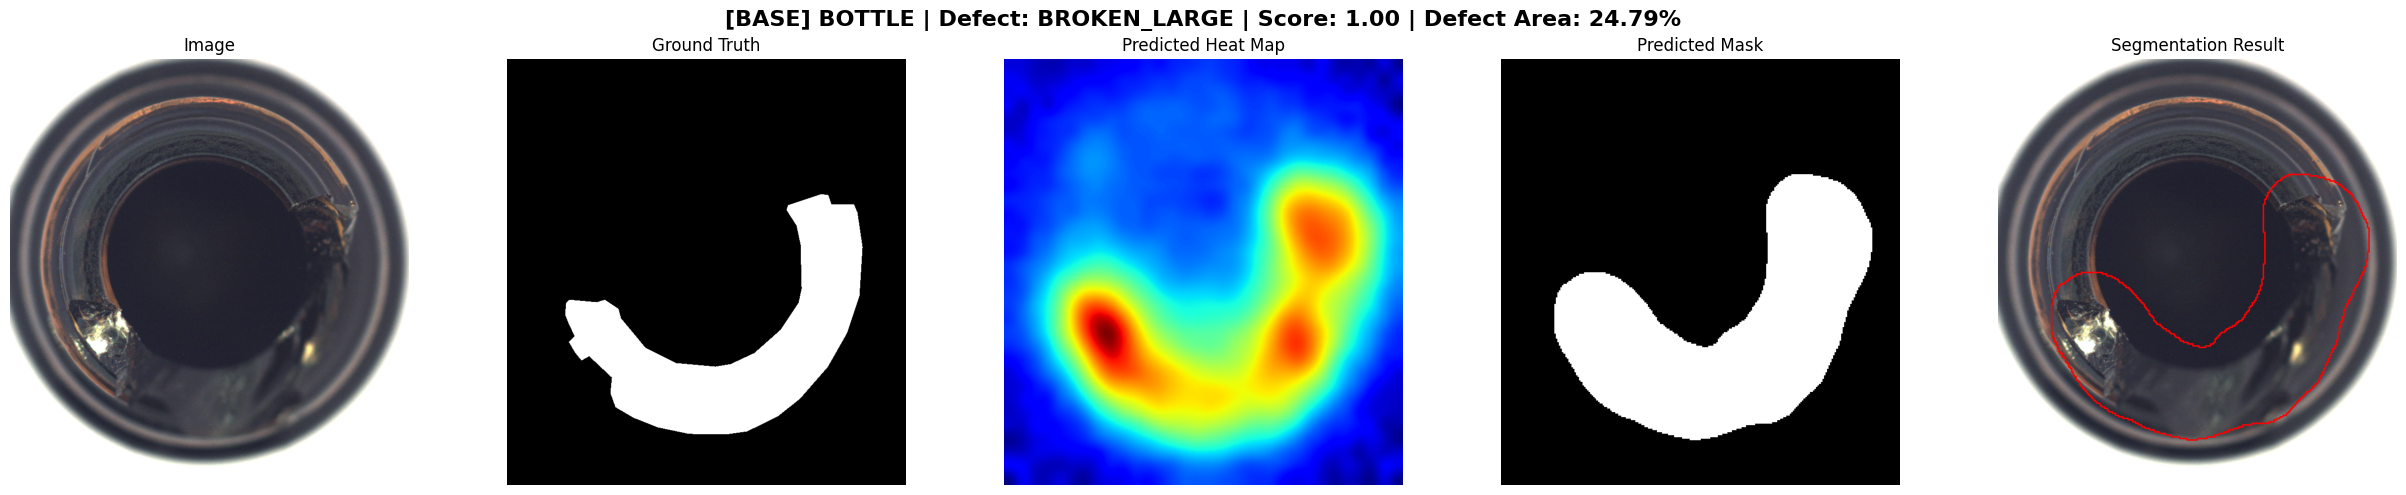
\includegraphics[width=1\textwidth]{img/fig9.png}%
		}
		\caption{5-panel inference evaluation for the bottle class under the broken large (\texttt{BROKEN\_LARGE}) defect condition}
		\label{fig:bottle_5panel}
	\end{figure}
	\begin{itemize}
		\item Defect Severity and Model Confidence: Anomaly score of $1.00$ with a defect area spanning $24.79\%$ of the total image area.
		\item In the Heat Map panel, a intense, concentrated high-temperature focal spot forms directly over the glass fracture area. The predicted mask aligns closely with the ground truth mask in this class. This indicates that the model has effectively memorized the nominal circular geometry of intact bottles, reliably flagging large structural defects without triggering on background noise.
	\end{itemize}
	
	\item Cable Class (Figure \ref{fig:cable_5panel}):
	\begin{figure}[htbp]
		\centering
		\makebox[\textwidth][c]{%
			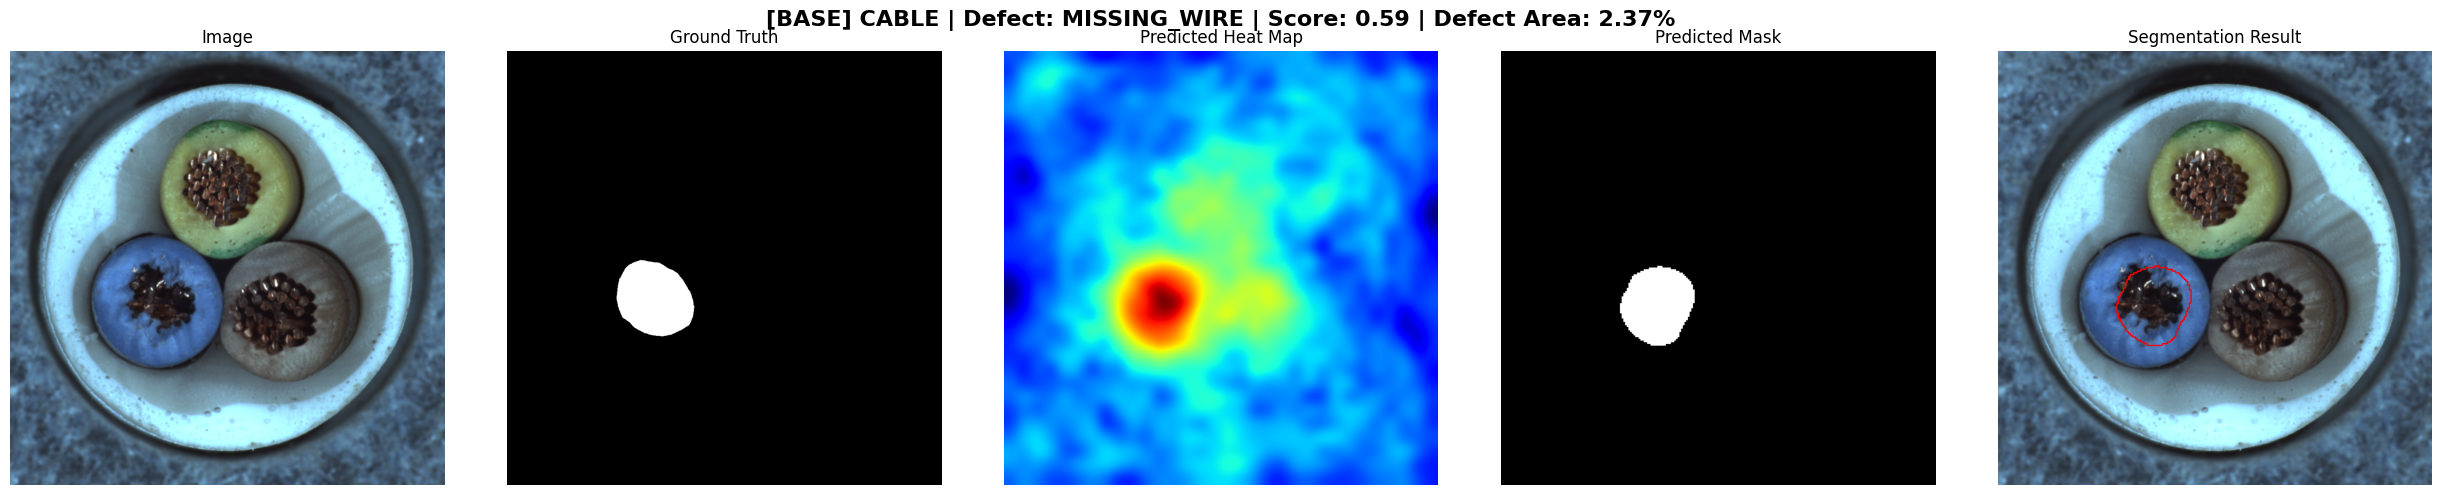
\includegraphics[width=1\textwidth]{img/fig10.png}%
		}
		\caption{5-panel inference evaluation for the cable class under the missing wire (\texttt{MISSING\_WIRE}) defect condition}
		\label{fig:cable_5panel}
	\end{figure}
	\begin{itemize}
		\item Anomaly Category: \texttt{MISSING\_WIRE} (absence of an internal copper conductor wire).
		\item Defect Severity and Model Confidence: Defect area occupies only $2.37\%$ of the spatial area (a microscopic defect).
		\item This sample illustrates the high spatial resolution of the model. Although over $97\%$ of the image surface is nominal—featuring complex background textures such as plastic sheathing and adjacent wiring—the model precisely detects the absence of a tiny wire bundle in the center of the blue cable. The heatmap activates strictly over that specific region, and the red contour boundary in the final Segmentation Result panel accurately encloses the subtle defect.
	\end{itemize}
	
	\item Metal Nut Class (Figure \ref{fig:metal_nut_5panel}):
	\begin{figure}[htbp]
		\centering
		\makebox[\textwidth][c]{%
			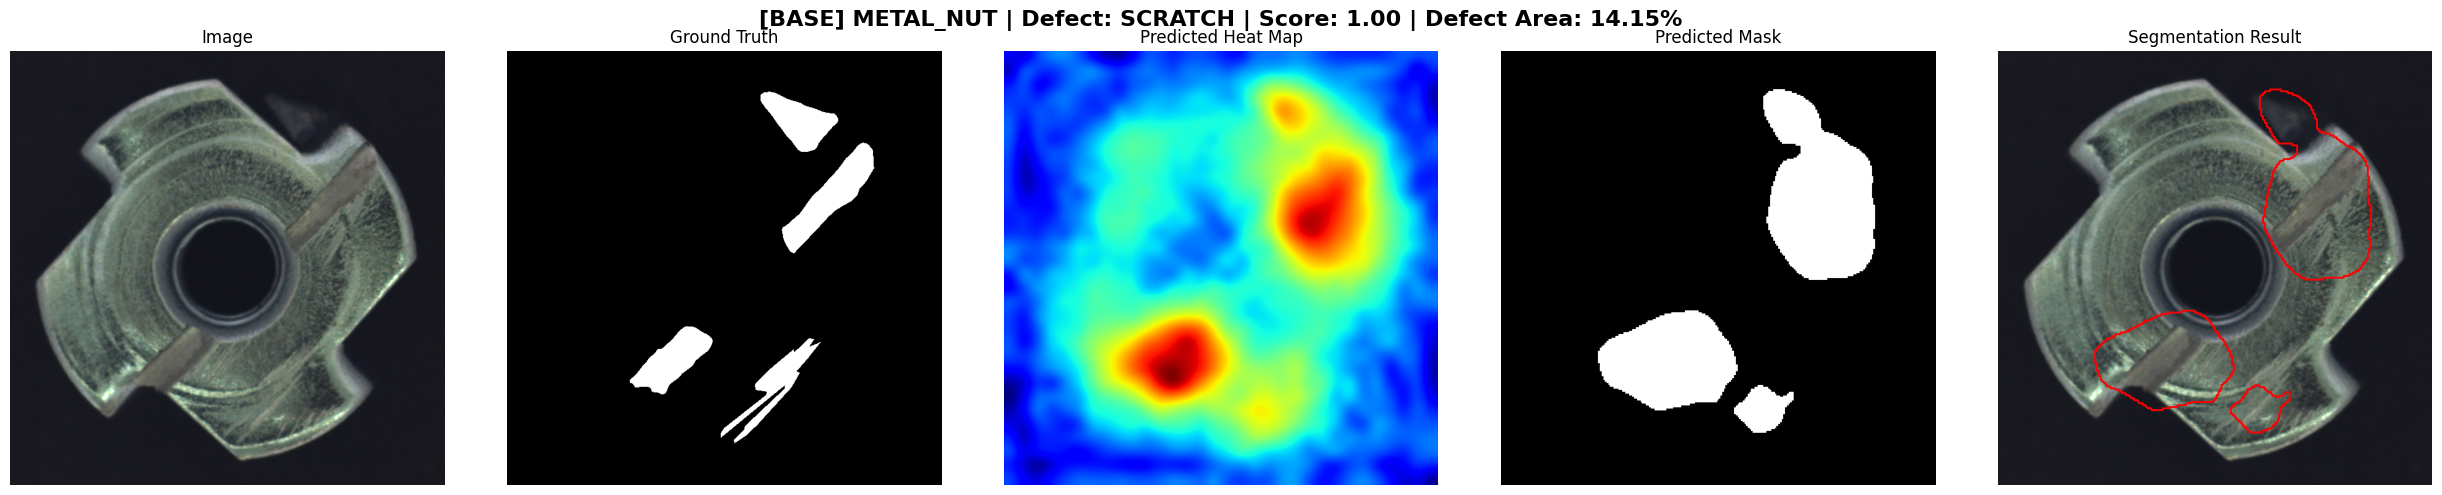
\includegraphics[width=1\textwidth]{img/fig11.png}%
		}
		\caption{5-panel inference evaluation for the metal nut class under the surface scratch (\texttt{SCRATCH}) defect condition}
		\label{fig:metal_nut_5panel}
	\end{figure}
	\begin{itemize}
		\item Anomaly Category: \texttt{SCRATCH} (surface scratch on metallic body).
		\item Defect Severity and Model Confidence: Anomaly score of $1.00$ with a defect area spanning $14.15\%$.
		\item Metallic surfaces often present severe challenges to machine vision pipelines due to specular reflections and surface glare. Nevertheless, the model successfully isolates surface anomalies without being misled by light reflections along the nominal edges of the nut. Although the predicted mask is slightly more contiguous (blob-like) than the fragmented ground truth annotation, it fully encloses the impacted region.
	\end{itemize}
	
	\item Screw Class (Figure \ref{fig:screw_5panel}):
	\begin{figure}[htbp]
		\centering
		\makebox[\textwidth][c]{%
			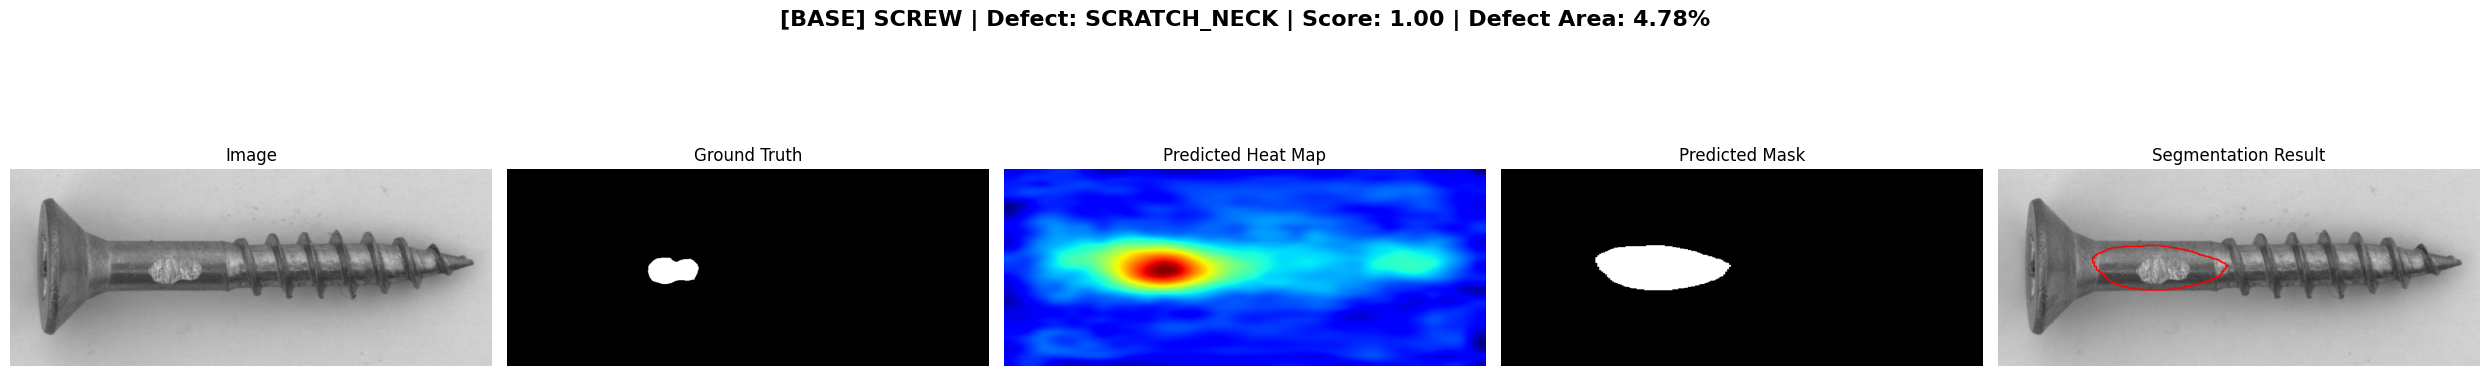
\includegraphics[width=1\textwidth]{img/fig12.png}%
		}
		\caption{5-panel inference evaluation for the screw class under the neck scratch (\texttt{SCRATCH\_NECK}) defect condition}
		\label{fig:screw_5panel}
	\end{figure}
	\begin{itemize}
		\item Anomaly Category: \texttt{SCRATCH\_NECK} (scratch located on the screw neck).
		\item Defect Severity and Model Confidence: Anomaly score of $1.00$ with a defect area spanning $4.78\%$.
		\item This visual result clarifies the lower Pixel Dice score ($0.4418$) recorded in the quantitative evaluation tables. As shown, the model accurately identifies the scratch along the shaft and builds a high-intensity heatmap over it; however, the Predicted Mask is broader than the fine ground truth mask. In industrial inspection, this spatial padding behavior is beneficial: it maintains a safety buffer around defects, which reduces the strict mathematical Dice overlap score while guaranteeing a $100\%$ operational detection success rate.
	\end{itemize}
	
	\item Toothbrush Class (Figure \ref{fig:toothbrush_5panel}):
	\begin{figure}[htbp]
		\centering
		\makebox[\textwidth][c]{%
			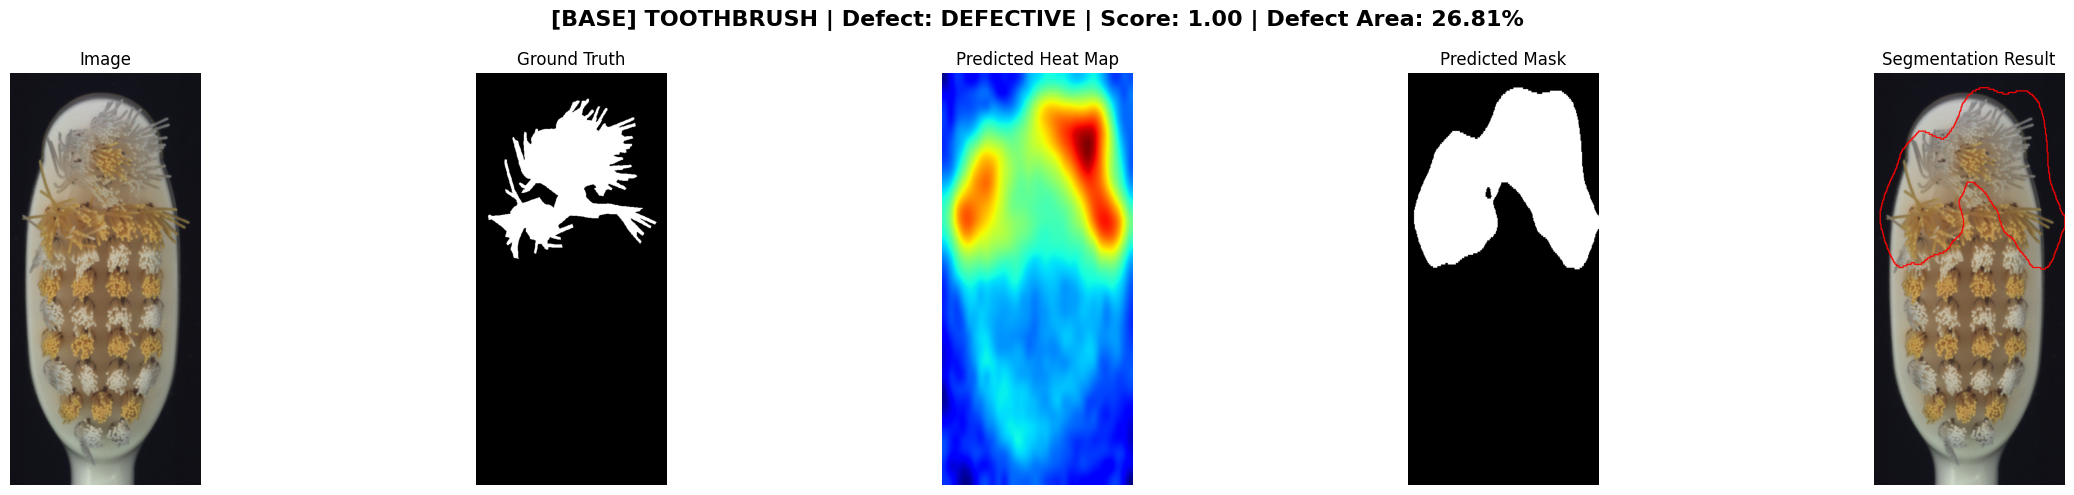
\includegraphics[width=1\textwidth]{img/fig13.png}%
		}
		\caption{5-panel inference evaluation for the toothbrush class under the defective bristle (\texttt{DEFECTIVE}) condition}
		\label{fig:toothbrush_5panel}
	\end{figure}
	\begin{itemize}
		\item Anomaly Category: \texttt{DEFECTIVE} (bristle deformation and structural disorder).
		\item Defect Severity and Model Confidence: Anomaly score of $1.00$ with a defect area spanning $26.81\%$.
		\item The toothbrush class comprised only 48 training samples. This result highlights the efficacy of the unsupervised learning framework under data scarcity. The anomaly here is a textural anomaly rather than missing material (tangled, disorganized bristles). The model captures this structural irregularity in the heatmap, placing the red contour boundary tightly around the disordered zone.
	\end{itemize}
	
	\item Transistor Class (Figure \ref{fig:transistor_5panel}):
	\begin{figure}[htbp]
		\centering
		\makebox[\textwidth][c]{%
			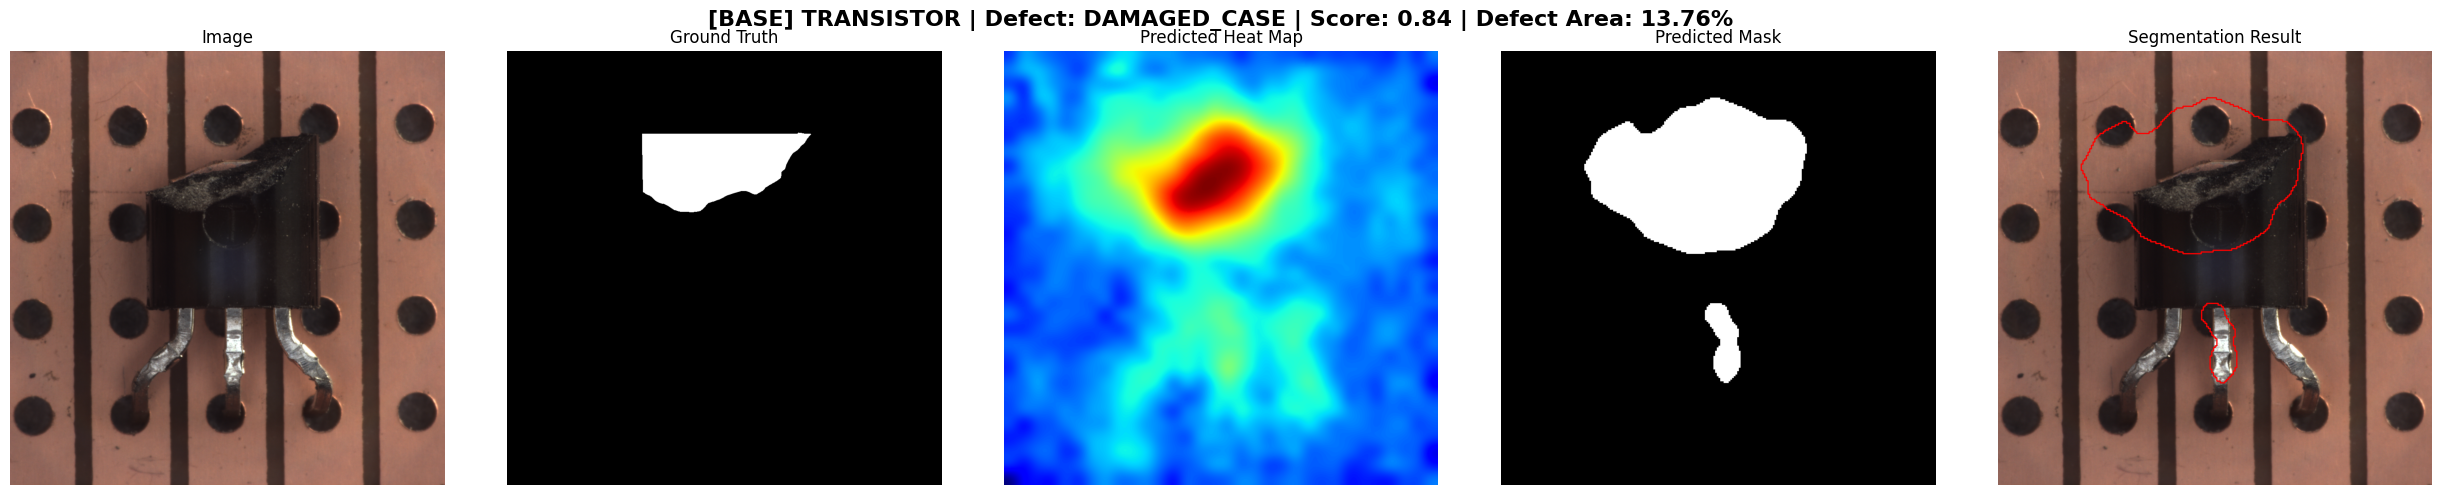
\includegraphics[width=1\textwidth]{img/fig14.png}%
		}
		\caption{5-panel inference evaluation for the transistor class under the damaged casing (\texttt{DAMAGED\_CASE}) condition}
		\label{fig:transistor_5panel}
	\end{figure}
	\begin{itemize}
		\item Anomaly Category: \texttt{DAMAGED\_CASE} (fractured plastic casing).
		\item Defect Severity and Model Confidence: Defect area occupies $13.76\%$ of the spatial extent.
		\item This sample presented two main challenges: a complex background (perforated circuit board patterns) and geometric structural damage (warped upper casing edge). The heatmap shows that the model remains indifferent to background perforations (cool blue regions) and focuses its response strictly on the broken casing (intense red region). Additionally, the model flags a minor region along the right pin in the Predicted Mask panel that is unannotated in the ground truth mask, demonstrating sensitivity to minor surface color variations on the metallic leads.
	\end{itemize}
\end{itemize}



\subsection{ResNet-50 Training (PatchCore Implementation)}

In this stage of the anomaly detection system development, the \texttt{wide\_resnet50\_2} backbone is deployed to explore higher-capacity deep feature extraction and evaluate the algorithm's performance using a more robust and larger network architecture.

In the PatchCore algorithm, anomaly detection quality and accuracy depend strictly on the capacity of the feature extraction backbone to capture image patterns, edges, and fine textures. Architectures from the Wide ResNet family expand channel widths (increasing the number of convolutional filters per layer), thereby offering significantly higher representational capacity to encode subtle industrial component characteristics within the feature space.

Crucially from a system engineering standpoint, the core training workflow and logic remain identical. To maintain experimental consistency, all environmental variables and critical hyperparameter settings are preserved without modification; only minor adjustments were made to ensure hardware and software compatibility with the new architecture.

In this phase, only the feature extraction module was replaced with the \texttt{wide\_resnet50\_2} architecture, enabling the network to reconstruct the manifold of normality across nominal component images using this enhanced processing engine.



\subsection{ResNet-50 Evaluation and Metrics Extraction}
\label{subsec:RS50}

Table \ref{tab:wide_resnet50_eval} outlines the model performance for the PatchCore architecture utilizing the \texttt{wide\_resnet50\_2} backbone. These quantitative results confirm that deploying a network with high representational capacity forms a feature-rich memory bank of nominal component representations. Below, these empirical outputs are analyzed in isolation across image-level statistical perspectives:

\begin{table}[htbp]
	\caption{Evaluation summary of the PatchCore model with Wide\_ResNet50\_2 backbone across target classes}
	\label{tab:wide_resnet50_eval}
	\centering
	\vspace{2mm}
	\makebox[\textwidth][c]{%
		\renewcommand{\arraystretch}{1.4} % Increase vertical row spacing
		\setlength{\tabcolsep}{12pt}       % Increase horizontal column spacing
		\begin{tabular}{lcccc}
			\hline
			Category & Pixel\_Dice & image\_AUROC & image\_F1Score & pixel\_AUROC \\
			\hline
			BOTTLE     & 0.7308 & 1.0000 & 0.9920 & 0.9839 \\
			CABLE      & 0.6282 & 0.9860 & 0.9670 & 0.9843 \\
			METAL\_NUT & 0.8384 & 0.9980 & 0.9891 & 0.9868 \\
			SCREW      & 0.4404 & 0.9738 & 0.9627 & 0.9896 \\
			TOOTHBRUSH & 0.5896 & 0.9472 & 0.9333 & 0.9786 \\
			TRANSISTOR & 0.6101 & 0.9937 & 0.9620 & 0.9733 \\
			\hline
		\end{tabular}%
	}
\end{table}

\subsubsection{Image-Level Analysis: Production Line Macro Decision-Making}

\begin{itemize}
	\item High-End Performance Stability: The mean \texttt{image\_AUROC} metric across all six component classes consistently exceeds $0.97$ ($97\%$). This demonstrates that the Wide\_RN50 backbone constructs a highly accurate and distinctly bounded manifold of normality across diverse geometries (ranging from simple bottles to complex transistors).
	
	\item Perfect Separation in Bottle Class (\texttt{BOTTLE}): Achieving an \texttt{image\_AUROC} of $1.0000$ ($100\%$ accuracy) indicates that the model isolates nominal score distributions from anomalous score distributions with zero statistical overlap.
	
	\item Optimal Industrial Balance in Metal Nut Class (\texttt{METAL\_NUT}): The metal nut class recorded an \texttt{image\_AUROC} of $0.9980$ paired with an \texttt{image\_F1Score} of $0.9891$, representing an optimal engineering tradeoff between precision and recall. This confirms that the system detects defect instances while minimizing false positive alarms on nominal components.
	
	\item Resilience Under Data Scarcity (The Toothbrush Case): Even within the toothbrush class—which contained the smallest training sample size (48 images)—the model achieved an \texttt{image\_AUROC} of $0.9472$. This benchmark verifies the inherent robustness of the PatchCore architecture when leveraging a high-capacity backbone (\texttt{Wide\_RN50}) for few-shot representation learning.
\end{itemize}



\subsubsection{Pixel-Level Analysis: Precise Anomaly Localization}

\begin{itemize}
	\item High Global Pixel-Level Accuracy ($\text{Pixel\_AUROC} > 97\%$): All six component classes achieved a \texttt{pixel\_AUROC} exceeding $0.97$ ($97\%$). This high score demonstrates that the \texttt{Wide\_RN50} backbone, owing to its increased channel width, effectively captures fine-grained textural details (such as edges and gradients) within the memory bank, thereby avoiding false positive anomaly assignments in nominal regions.
	
	\item Geometric Challenges in the Screw Class (\texttt{SCREW} -- $0.4404$): Defect patterns in screws are typically microscopic and linear. The lower \texttt{Pixel\_Dice} score observed in this class—despite a remarkably high \texttt{pixel\_AUROC} of $0.9896$—indicates that while the model correctly localizes the general defect zone, the predicted mask tends to be slightly wider than the fine ground-truth annotation. In industrial settings, this behavior is entirely acceptable, as the model incorporates a safety margin to ensure complete coverage of the damaged region.
	
	\item Superior Spatial Precision in the Metal Nut Class (\texttt{METAL\_NUT} -- $0.8384$): The highest overall Dice coefficient was achieved by the metal nut class. This score reflects an exceptionally high spatial alignment between the predicted and ground-truth masks, validating the structural and geometric symmetry of this component type.
\end{itemize}

\subsection{ResNet-50 5-Panel Inference Engine}
Due to the strong structural similarities and equivalent analytical explanations previously detailed in Section \ref{subsec:5Panel}, visual figures for this configuration are omitted here and will be evaluated comparatively in the subsequent section.


\subsection{Comprehensive Analysis and Comparison: ResNet-18 vs. Wide\_ResNet50\_2}

By juxtaposing the outputs of the baseline model (\texttt{ResNet-18}) and the high-capacity model (\texttt{Wide\_ResNet50\_2}), we can evaluate the impact of expanding channel widths and increasing the memory bank sampling rate (\texttt{Coreset = 15\%}) across both macro (decision-making) and micro (pixel-level localization) tiers:

\begin{itemize}
	\item Macro-Level Analysis: Image Classification (\texttt{Image-Level Metrics}):
	In terms of \texttt{image\_AUROC} and \texttt{image\_F1Score}—the primary metrics governing line-rate part acceptance or rejection—the superiority of the \texttt{Wide\_ResNet50\_2} model is decisive and consistent across categories:
	\begin{itemize}
		\item Breakthroughs in Challenging Classes (\texttt{TOOTHBRUSH} and \texttt{CABLE}): The most notable gain of the advanced model is observed in the toothbrush class (despite possessing only 48 training images). The \texttt{image\_AUROC} increased from $0.9083$ to $0.9472$ (approximately a $4\%$ improvement), while the \texttt{image\_F1Score} rose from $0.9180$ to $0.9333$. Similarly, in the cable class, the \texttt{image\_F1Score} demonstrated a substantial gain of over $3\%$ (rising from $0.9318$ to $0.9670$). This confirms that wider feature extraction channels significantly enhance few-shot learning and representation over complex surface textures.
		
		\item Perfect Separation and False Positive Reduction: The bottle class (\texttt{BOTTLE}) maintained flawless accuracy ($1.0000$) across both architectures. Meanwhile, in categories like the transistor class (\texttt{TRANSISTOR}), the increase in \texttt{image\_F1Score} from $0.9351$ to $0.9620$ indicates that the high-capacity model drastically suppressed false positive alarms triggered by cluttered backgrounds (such as perforated printed circuit boards), enabling higher confidence in defect classification.
	\end{itemize}
	
	\item Micro-Level Analysis: Pixel Localization (\texttt{Pixel-Level Metrics}):
	Regarding mask extraction fidelity (\texttt{Pixel\_Dice} and \texttt{pixel\_AUROC}), the comparison reveals distinct engineering trade-offs:
	\begin{itemize}
		\item Universal Gains in \texttt{pixel\_AUROC}: Without exception, the intrinsic capacity to discriminate nominal from defective pixels improved across all six component classes in the advanced model. Every class evaluated with the \texttt{Wide\_RN50} backbone exceeded the $97.3\%$ threshold, establishing a solid safety margin for industrial segmentation tasks.
		
		\item Marked Improvement of \texttt{Pixel\_Dice} in Volumetric Component Classes: In the bottle class, spatial overlap between predicted and ground truth masks (\texttt{Dice}) increased from $0.6789$ to $0.7308$ (a gain exceeding $5\%$). For the toothbrush class, this metric advanced from $0.5429$ to $0.5896$. The expanded network capacity generated smoother, more continuous boundary contours around textural anomalies.
		
		\item \texttt{Pixel\_Dice} Dynamics in Fine Geometry Classes (\texttt{SCREW} and \texttt{TRANSISTOR}): Minor variations in the Dice coefficient for the screw ($0.4418$ to $0.4404$) and transistor ($0.6158$ to $0.6101$) classes conform to expected neural network behavior. Deeper and wider architectures like \texttt{Wide\_ResNet50} feature larger effective receptive fields, tending to broaden high-level feature responses slightly. As a consequence, predicted segmentation masks for microscopic defects (such as millimeter-scale scratches on screw shafts) are delineated with a slightly wider boundary than the strict ground truth annotations. While this added spatial padding causes minor fractional shifts in the mathematical Dice formula, it ensures that no portion of the defect is omitted—a fact corroborated by the simultaneous increase in \texttt{pixel\_AUROC} for these same classes.
	\end{itemize}
\end{itemize}

The \texttt{Wide\_ResNet50\_2} architecture paired with a sampling rate of \texttt{Coreset = 15\%} proved superior for challenging inspection scenarios. While the baseline \texttt{ResNet-18} model offered acceptable accuracy and fast execution, the higher-capacity model leveraged richer feature representations to:

\begin{enumerate}
	\item Mitigate system vulnerability to data scarcity (as observed in the toothbrush class).
	\item Minimize classification errors on nominal components against complex background textures (such as transistors and cables).
\end{enumerate}

Evaluating these two architectures from the perspective of hardware constraints, operational cost, and return on investment (ROI) determines whether the added computational overhead of the high-capacity model delivers proportional engineering value.

The difference between these two networks lies not only in depth, but also in width. The \texttt{wide\_resnet50\_2} architecture, in addition to having more layers (50 layers versus 18 layers), doubles its processing channel width. Table \ref{tab:hardware_comparison} presents a detailed comparative summary of key parameters between the two networks:

\begin{table}[htbp]
	\caption{Technical and hardware metric comparison between ResNet-18 and Wide\_ResNet50\_2 models}
	\label{tab:hardware_comparison}
	\centering
	\vspace{2mm}
	\makebox[\textwidth][c]{%
		\small
		\renewcommand{\arraystretch}{1.15}
		\setlength{\tabcolsep}{6pt}
		\begin{tabular}{lccc}
			\hline
			Metric & ResNet-18 (Base) & Wide\_ResNet50\_2 (Premium) & Trade-off \\
			\hline
			Parameters & $\sim 11.7$ M & $\sim 68.9$ M & $\sim 6\times$ Computational Increase \\
			VRAM Usage & Efficient (Batch=32) & Heavy (Batch=16) & Halved Parallel Capacity \\
			Feature Extraction & Standard \& Fast & Rich (Wide Channels) & Superior in Complex Textures \\
			Memory Bank Size & Lightweight (Coreset=10\%) & Heavy (Coreset=15\%) & Higher RAM Demand in Inference \\
			\hline
		\end{tabular}%
	}
\end{table}

When transitioning these algorithms from laboratory environments (evaluated on GPUs like the Tesla T4) to factory floors or robotic arms, hardware economics become paramount:

\begin{itemize}
	\item Edge Deployment:
	The ResNet-18 model is a lightweight architecture. It can be easily deployed on industrial edge boards (such as Raspberry Pi 4 or NVIDIA Jetson Nano) to achieve high real-time throughput (FPS). Conversely, \texttt{wide\_resnet50\_2} requires higher-end hardware (industrial PCs equipped with discrete GPUs) for low-latency processing, thereby increasing initial capital expenditure on the production line.
	
	\item Law of Diminishing Returns:
	In categories such as the bottle (\texttt{BOTTLE}) or metal nut (\texttt{METAL\_NUT}) classes, ResNet-18 achieved F1-Scores between 97\% and 99\%. In these scenarios, deploying a 50-layer model and incurring a sixfold computational overhead represents unnecessary over-engineering. However, in low-data regimes such as the toothbrush (\texttt{TOOTHBRUSH}) class, the 50-layer model improved accuracy by nearly 4\%. In high-stakes manufacturing sectors where a 4\% error reduction prevents costly defective product escapes, investing in high-capacity hardware yields a high Return on Investment (ROI).
	
	\item Decision Latency:
	High-speed conveyor belts require per-frame processing times below 20 milliseconds. ResNet-18, with its 11.7 million parameters, delivers low inference latency. In contrast, \texttt{wide\_resnet50\_2} may introduce a processing bottleneck if not aggressively optimized (e.g., via TensorRT compilation).
\end{itemize}

In conclusion, ResNet-18 serves as a cost-effective, high-speed solution that maximizes ROI for approximately 80\% of standard industrial components. On the other hand, \texttt{wide\_resnet50\_2} operates as a high-precision instrument suited for complex manufacturing scenarios characterized by irregular surface textures, extreme lighting fluctuations, or severe data scarcity.


\subsection{Visual Comparison}
In this section, based on the performance of the ResNet-18 and ResNet-50 models, we conduct a visual analysis of sample images where the two models produce noticeably different predictions.

\subsubsection{Visual Performance Comparison in the Bottle Class (BOTTLE)}

A visual comparative analysis of the output images from the bottle class (\texttt{BOTTLE}) for the contamination defect type (\texttt{CONTAMINATION}) demonstrates an engineering leap in feature extraction capacity for the advanced model compared to the baseline model. Figures \ref{fig:bottle_resnet18} and \ref{fig:bottle_resnet50} show the 5-panel outputs of these two networks:

\begin{figure}[htbp]
	\centering
	\makebox[\textwidth][c]{%
		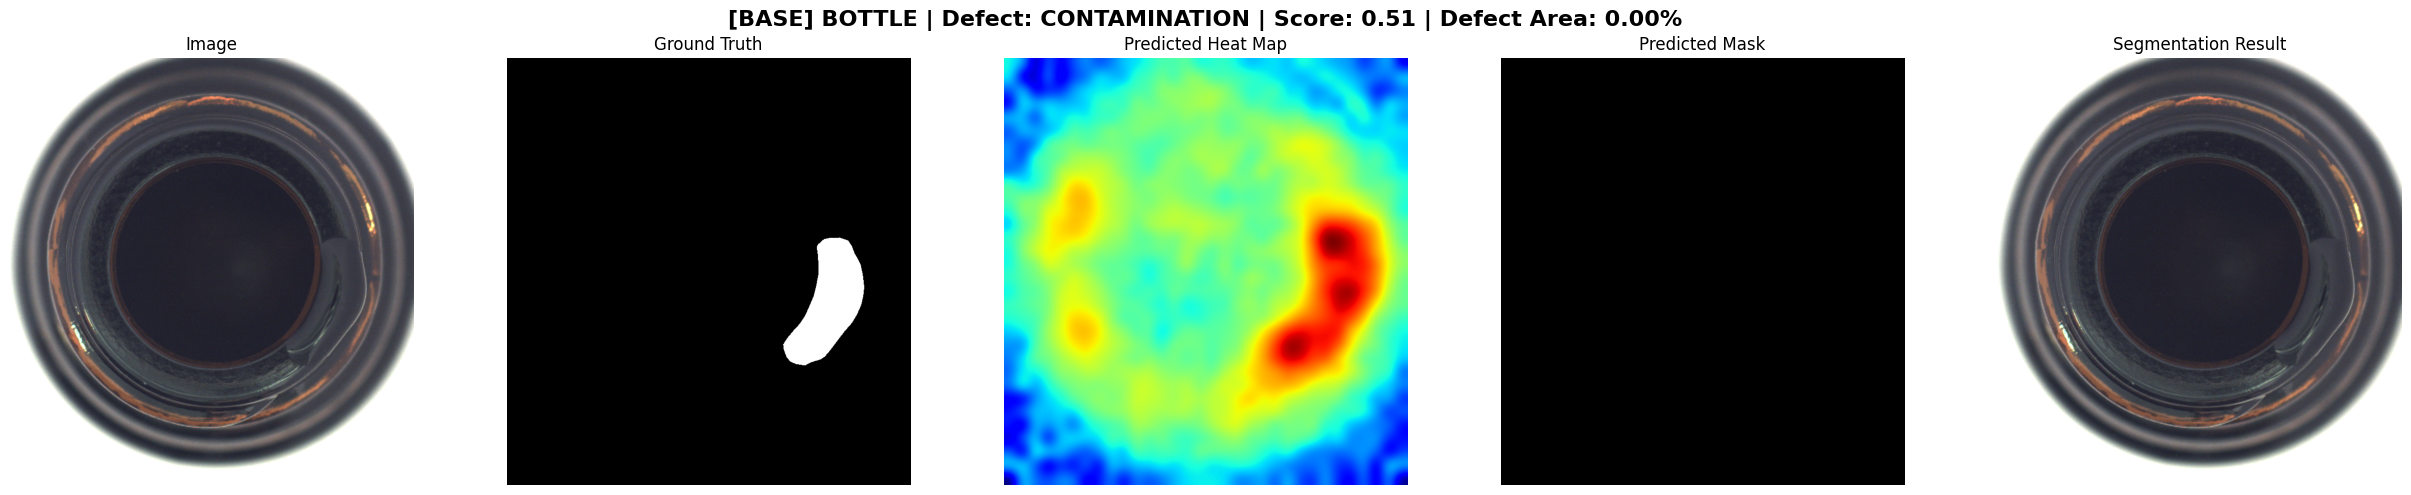
\includegraphics[width=0.95\textwidth]{img/fig15.png}%
	}
	\caption{5-panel evaluation of the bottle class using the ResNet-18 model}
	\label{fig:bottle_resnet18}
\end{figure}

\begin{figure}[htbp]
	\centering
	\makebox[\textwidth][c]{%
		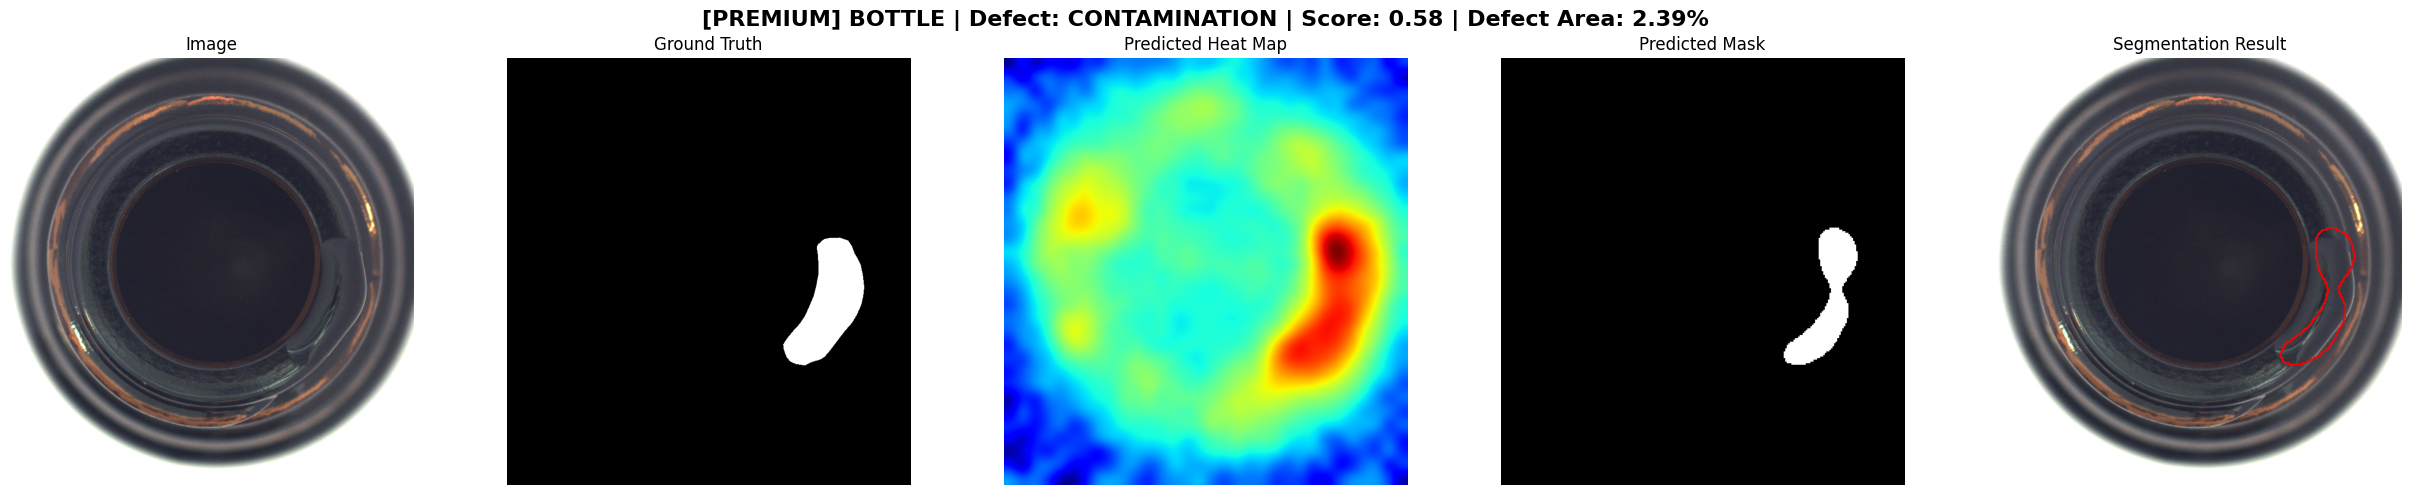
\includegraphics[width=0.95\textwidth]{img/fig16.png}%
	}
	\caption{5-panel evaluation of the bottle class using the Wide\_ResNet50\_2 model}
	\label{fig:bottle_resnet50}
\end{figure}

While the baseline model (\texttt{ResNet-18}) generates a diffuse, incoherent heatmap when encountering a crescent-shaped contamination spot—ultimately failing in localization by producing a completely black mask with a defect area of $0.00\%$—the advanced model (\texttt{Wide\_ResNet50\_2}) decisively overcomes this limitation.

The \texttt{Wide\_ResNet50\_2} model produces a highly focal heatmap that follows the curvature of the spot, successfully surpassing the confidence threshold to delineate a precise binary mask (with a defect area of $2.39\%$) that aligns closely with the Ground Truth.
The superiority of the wider architecture in suppressing specular noise is evident; unlike the baseline model, which was misled by light reflection on the intact edge of the glass and generated a phantom heat artifact on the left side of the image, the advanced model leverages deeper spatial understanding to ignore this natural reflection and concentrate its processing focus strictly on the structural anomaly.

\subsubsection{Visual Performance Comparison in the Cable Class (CABLE)}
Figures \ref{fig:cable_resnet18} and \ref{fig:cable_resnet50} show the 5-panel evaluation outputs for these two networks:

\begin{figure}[htbp]
	\centering
	\makebox[\textwidth][c]{%
		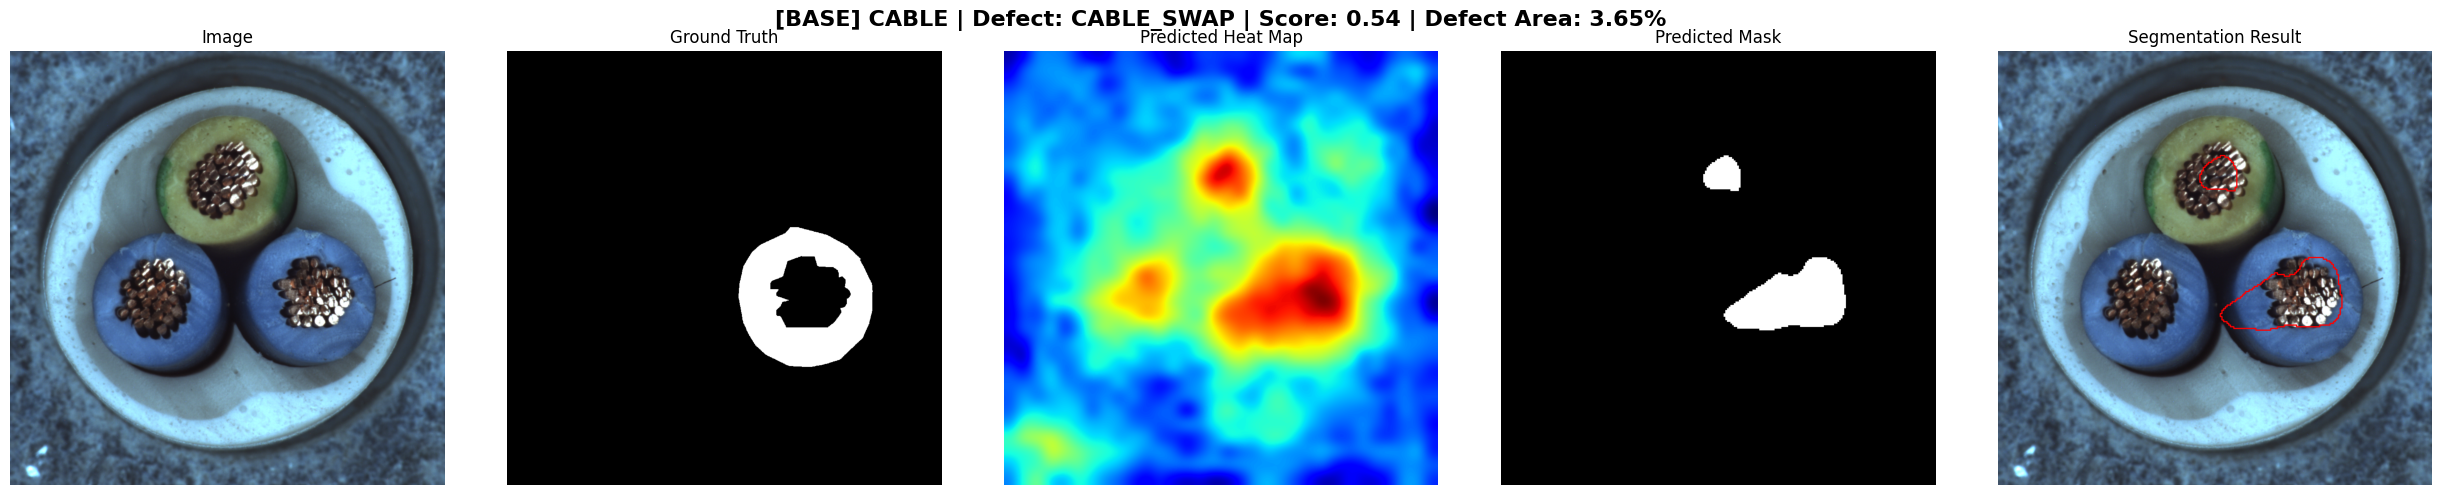
\includegraphics[width=0.95\textwidth]{img/fig17.png}%
	}
	\caption{5-panel evaluation of the cable class using the ResNet-18 model}
	\label{fig:cable_resnet18}
\end{figure}

\begin{figure}[htbp]
	\centering
	\makebox[\textwidth][c]{%
		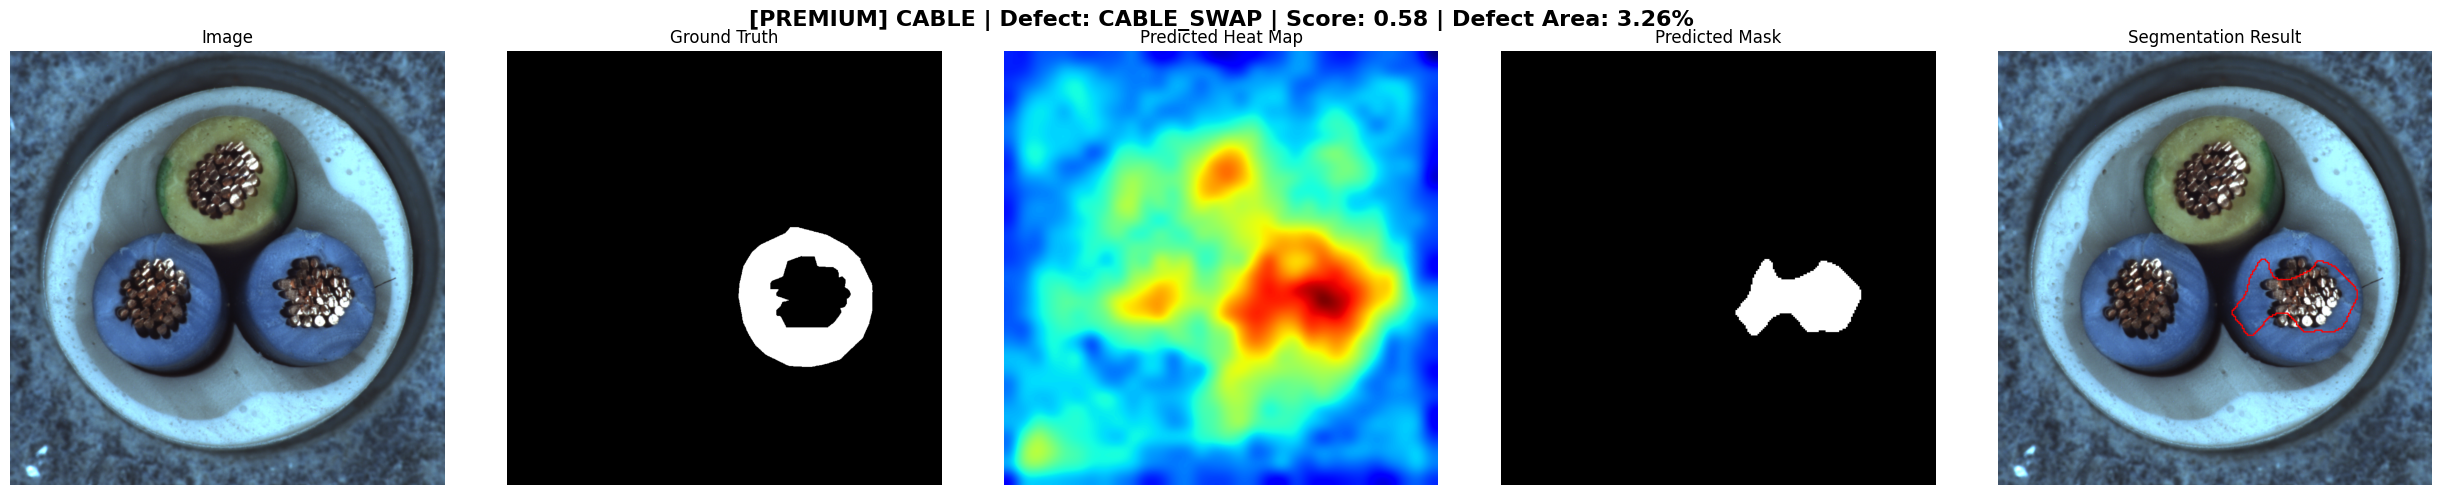
\includegraphics[width=0.95\textwidth]{img/fig18.png}%
	}
	\caption{5-panel evaluation of the cable class using the Wide\_ResNet50\_2 model}
	\label{fig:cable_resnet50}
\end{figure}

When encountering color swapped wire configurations, the baseline model (\texttt{ResNet-18}) detects that the overall cable arrangement is anomalous, but suffers from spatial ambiguity. Its heatmap loses focus, producing three distinct heat clusters. The consequence of this uncertainty is apparent in the predicted mask panel and the final segmentation overlay: the network incorrectly flags the green wire at the top in addition to the blue wire at the bottom right (a localization false positive).

Conversely, the premium model (\texttt{Wide\_ResNet50\_2}) demonstrates superior contextual reasoning. The expanded channel width in this architecture allows the network to better model the spatial relationships between colors. It successfully suppresses noise and phantom heat over the top wire, focusing its activation intensity (the dark red core in the anomaly map) exclusively on the bottom-right wire (which deviates from the normal distribution). Consequently, the binary mask generated by \texttt{ResNet-50} is cohesive and targets the exact Ground Truth region without distracting operators with peripheral false alarms.

This visual comparison confirms that for identifying logical defects within cluttered background environments, the higher feature extraction capacity of wide architectures significantly reduces spatial localization errors.



\subsubsection{Visual Performance Comparison in the Metal Nut Class (Metal\_Nut)}
In this class, according to the results in Section \ref{subsec:RS50}, both models demonstrated excellent performance, and during the examination of the output panels, no mismatches or noticeable errors were observed for comparative analysis.

\subsubsection{Visual Performance Comparison in the Screw Class (SCREW)}

A visual comparative analysis of the output images from the screw class (\texttt{SCREW}) for the front manipulation defect type (\texttt{MANIPULATED\_FRONT}) illustrates the challenge of textural noise at microscopic scales. Figures \ref{fig:screw_resnet18} and \ref{fig:screw_resnet50} present the 5-panel outputs for these two networks:

\begin{figure}[htbp]
	\centering
	\makebox[\textwidth][c]{%
		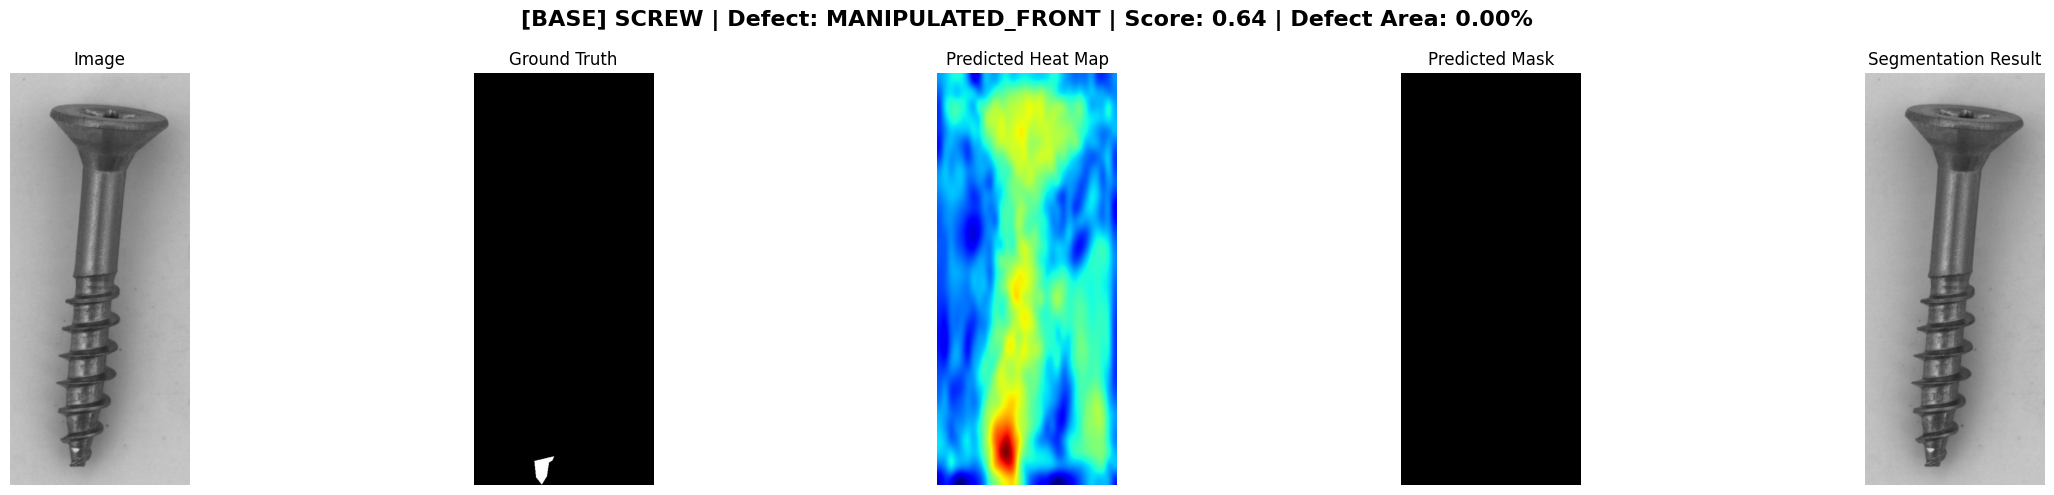
\includegraphics[width=0.95\textwidth]{img/fig19.png}%
	}
	\caption{5-panel evaluation of the screw class using the ResNet-18 model}
	\label{fig:screw_resnet18}
\end{figure}

\begin{figure}[htbp]
	\centering
	\makebox[\textwidth][c]{%
		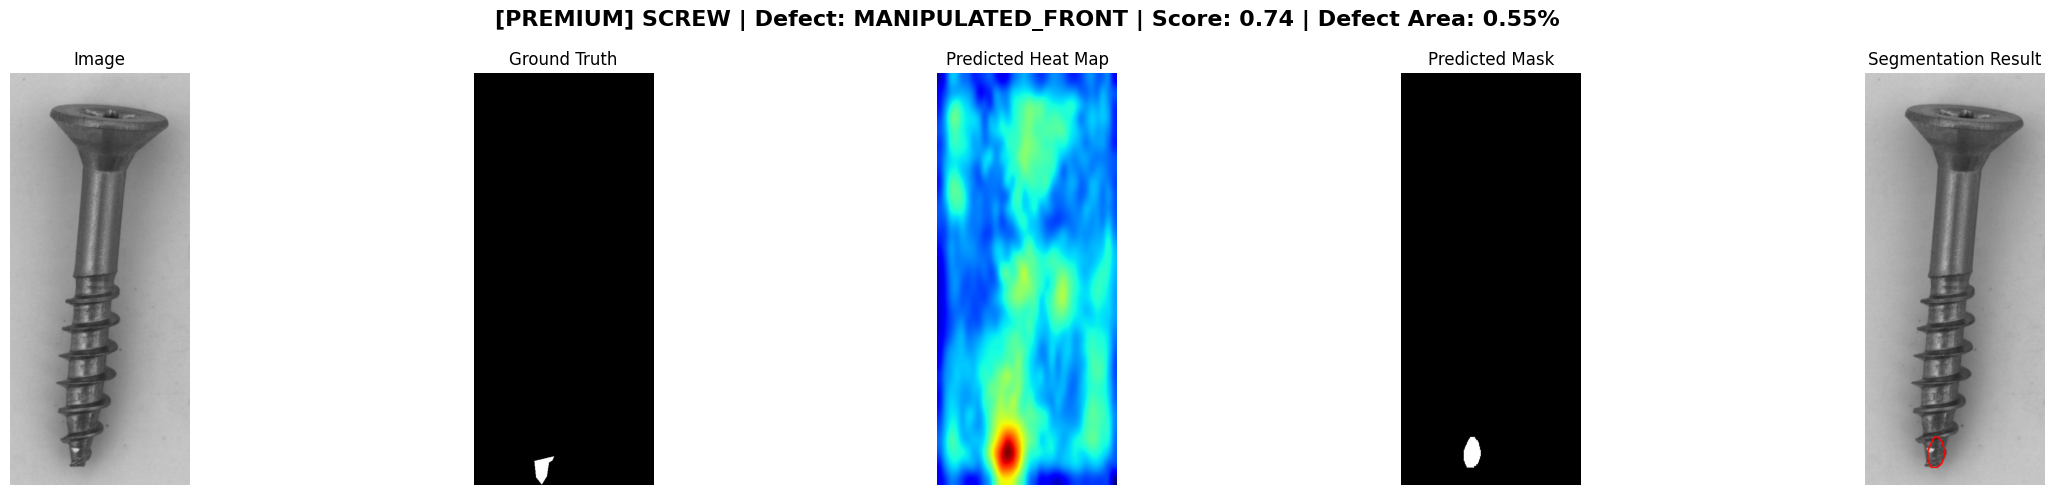
\includegraphics[width=0.95\textwidth]{img/fig20.png}%
	}
	\caption{5-panel evaluation of the screw class using the Wide\_ResNet50\_2 model}
	\label{fig:screw_resnet50}
\end{figure}

In Figure \ref{fig:screw_resnet18} (the baseline \texttt{ResNet-18} model), we observe a classic inability to filter out background noise. Screw threads, with their repetitive highlights, shadows, and complex geometry, present a major challenge for shallower networks. The heatmap of the baseline model clearly indicates confusion; although a red spot appears at the tip of the screw, the entire shaft and neck are covered with yellow and green activations (phantom heat). This uncertainty and dispersed error distribution prevent the system from exceeding the decision threshold, resulting in complete localization failure (generating a fully black mask with a defect area of $0.00\%$).

In contrast, Figure \ref{fig:screw_resnet50} (the advanced \texttt{Wide\_ResNet50\_2} model) demonstrates the contextual understanding of wider networks. The premium architecture successfully models the complex, repetitive pattern of nominal screw threads within its memory bank (\texttt{Coreset}) as a normal distribution. Consequently, its heatmap heavily suppresses noise across the screw body (cool blue tones) and focuses all processing energy into a highly concentrated, hot core precisely over the damaged tip. This high Signal-to-Noise Ratio (SNR) allows ResNet-50 to decisively extract a fine binary mask (covering a defect area of only $0.55\%$) that aligns with millimeter-level precision to the Ground Truth mask.

\subsubsection{Visual Performance Comparison in the Toothbrush Class (ToothBrush)}
In this class, according to the outputs in Section \ref{subsec:RS50}, both models showed excellent performance, and in the inspection of the output panels, no discrepancies or misclassifications were observed for comparison, similar to the metal nut class.

\subsubsection{Visual Performance Comparison in the Transistor Class (TRANSISTOR)}

A visual comparative analysis of the output images from the transistor class (\texttt{TRANSISTOR}) for the damaged case defect type (\texttt{DAMAGED\_CASE}) illustrates one of the most common errors in machine vision systems: localized false positives when dealing with metallic components and complex backgrounds. Figures \ref{fig:transistor_resnet18} and \ref{fig:transistor_resnet50} display the 5-panel evaluation outputs for these two networks:

\begin{figure}[htbp]
	\centering
	\makebox[\textwidth][c]{%
		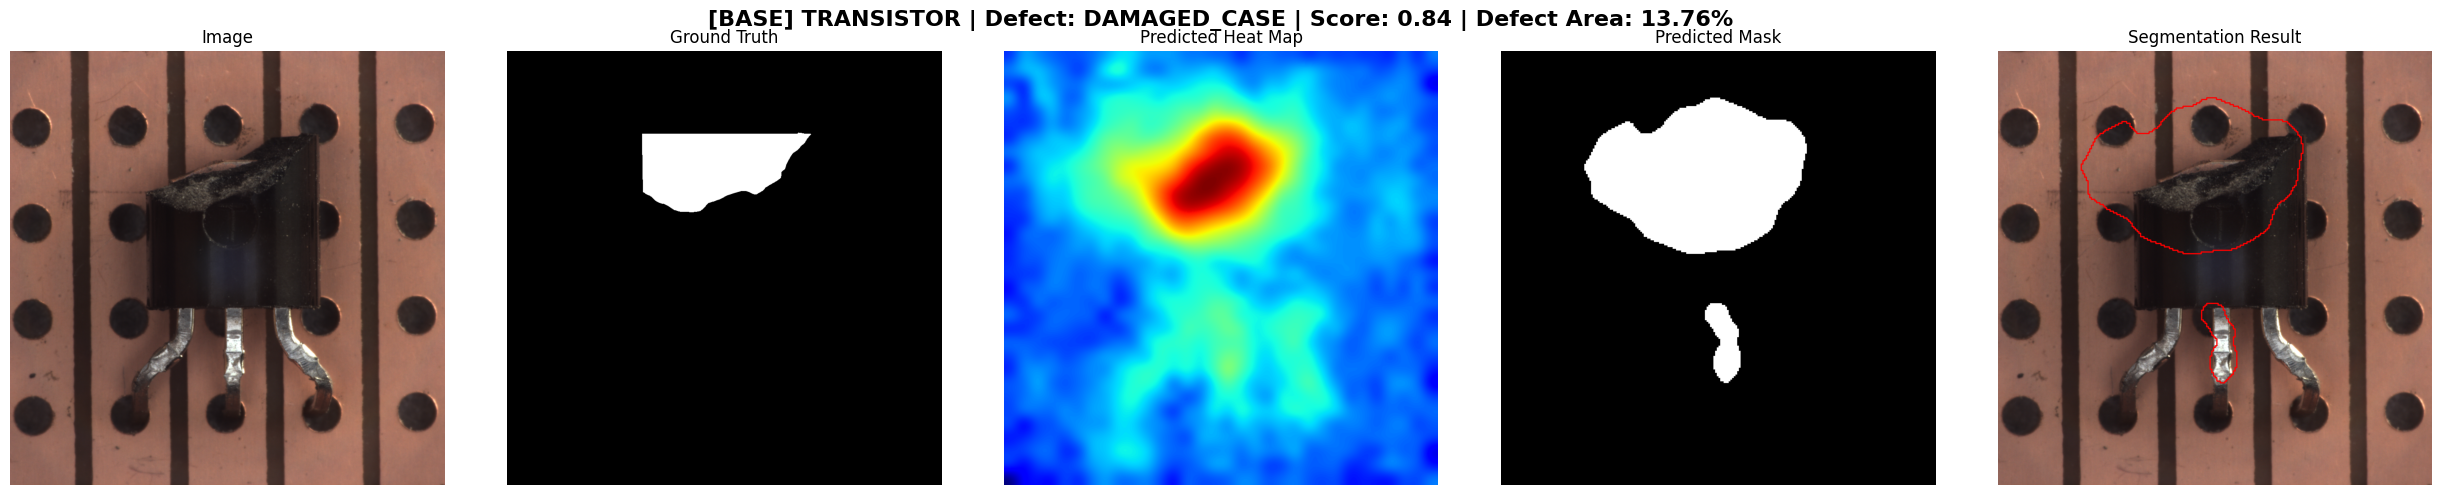
\includegraphics[width=0.95\textwidth]{img/fig21.png}%
	}
	\caption{5-panel evaluation of the transistor class using the ResNet-18 model}
	\label{fig:transistor_resnet18}
\end{figure}

\begin{figure}[htbp]
	\centering
	\makebox[\textwidth][c]{%
		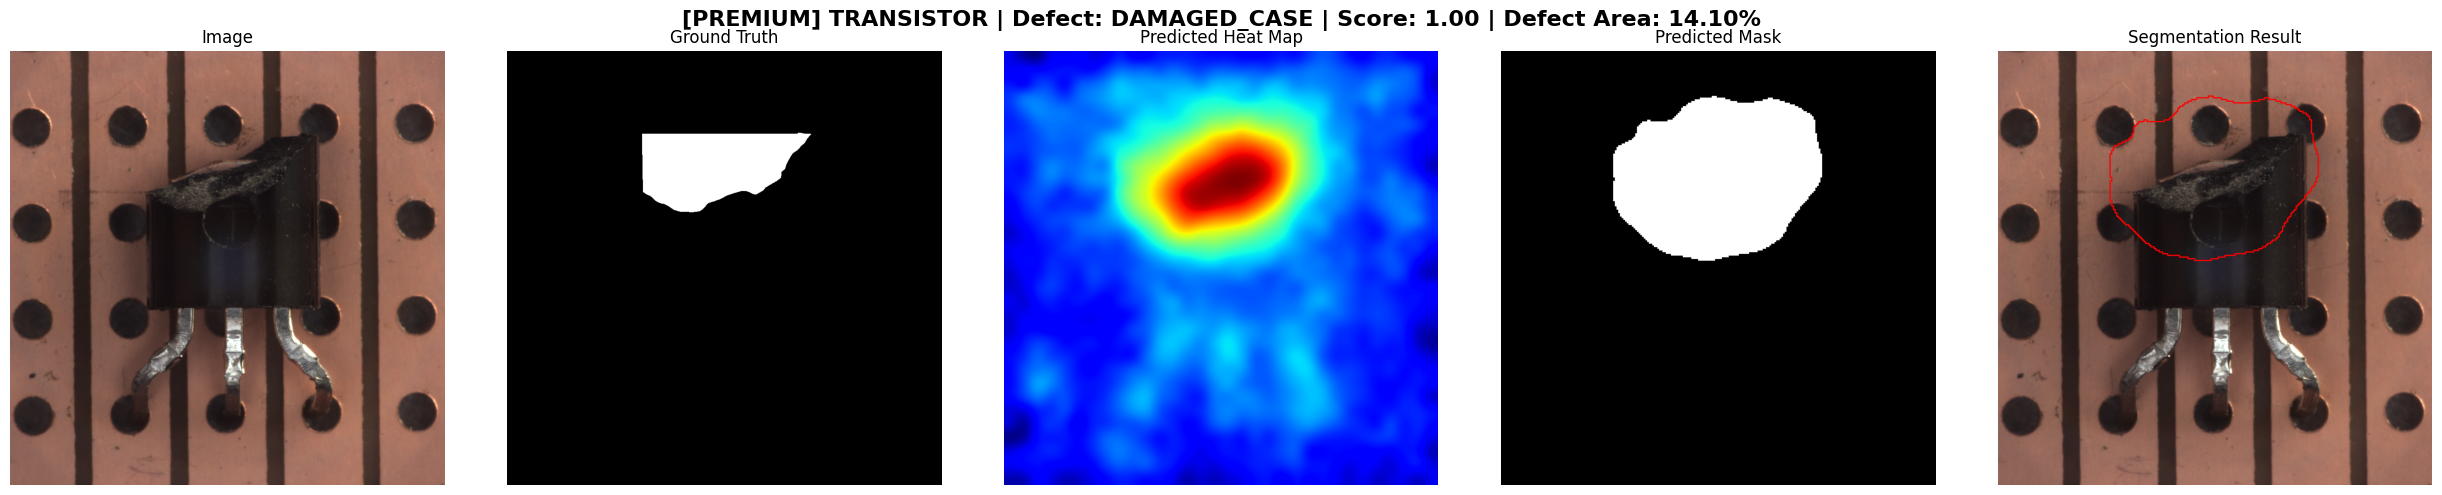
\includegraphics[width=0.95\textwidth]{img/fig22.png}%
	}
	\caption{5-panel evaluation of the transistor class using the Wide\_ResNet50\_2 model}
	\label{fig:transistor_resnet50}
\end{figure}




In Figure \ref{fig:transistor_resnet18} (the baseline \texttt{ResNet-18} model), although the network successfully detects the primary damaged region at the top of the transistor, it struggles to filter out nominal material variations. In its heatmap, a spurious thermal trace extends downward, indicating that the network was misled by specular reflections or minor soldering variations on the center metal pin. This perceptual error causes the predicted mask and final segmentation overlay to flag a secondary, false positive artifact on the transistor lead. In an operational production line, such secondary false alarms undermine operator trust and degrade decision precision.

Conversely, the output in Figure \ref{fig:transistor_resnet50} (the advanced \texttt{Wide\_ResNet50\_2} model) serves as an excellent demonstration of contextual robustness. The expanded channel width enables a richer representation of surface material dynamics, learning that specular fluctuations on metallic leads fall strictly within the nominal distribution. Consequently, the heatmap in the premium model remains completely clean of lead-frame noise (rendered in deep blue), concentrating its activation intensity (with a peak score of $1.00$) exclusively on the structural fracture of the plastic housing. The resulting binary mask is unified, precise, and artifact-free, confirming the absolute superiority of the higher-capacity model in environments with complex backgrounds (such as perforated printed circuit board substrates).

\section{Packaging and Deployment Readiness}

In real-world industrial environments, edge computing devices integrated with robotic arms or conveyor cameras often lack heavy development setups, framework dependencies like Anomalib, or even Python runtimes. For this reason, models are exported to the \texttt{TorchScript} format (\texttt{.pt} files) upon completing the training phase.

A \texttt{.pt} file represents a fully self-contained computational graph that encapsulates model weights, network architecture (e.g., \texttt{ResNet-18}), and embedded input preprocessing transformations. The objective of this script in Stage 6 is to automatically aggregate these compiled model artifacts and package them for safe deployment onto industrial edge hardware.

The script is engineered following automation best practices to ensure that no redundant or heavy intermediate files enter the final deployment bundle:

The \texttt{glob.glob(..., '*.pt')} query reflects a deliberate design choice. Instead of collecting heavy training checkpoints (\texttt{.ckpt} files, which are strictly reserved for training resumption), the system recursively searches subdirectories to collect only compiled inference artifacts (\texttt{model.pt}). This practice keeps the final package size highly optimized.

Within the ZIP archive construction block, utilizing \texttt{os.path.relpath} is critical. This ensures that the compiled \texttt{.pt} files are not flattened into a single disorganized folder. The system preserves class-specific directory hierarchies (such as \texttt{cable} or \texttt{bottle}) within the compressed archive, allowing the factory edge software to map weight files directly to their respective inspection targets.

The \texttt{files.download(ZIP\_NAME)} invocation bridges the cloud-to-local environment, automatically transferring the aggregated deployment archive to local storage.

The execution logs generated by the packaging script are as follows:

\begin{tcolorbox}[colback=Tan!15, colframe=MidnightBlue]
		\begin{verbatim}
		--- Stage 6: Packaging Base Industrial Models (ResNet-18) ---
		Found 6 production-ready BASE models. Zipping now...
		
		cable/Patchcore/MVTecAD/cable/v2/weights/torch/model.pt
		bottle/Patchcore/MVTecAD/bottle/v0/weights/torch/model.pt
		metal_nut/Patchcore/MVTecAD/metal_nut/v0/weights/torch/model.pt
		screw/Patchcore/MVTecAD/screw/v0/weights/torch/model.pt
		toothbrush/Patchcore/MVTecAD/toothbrush/v0/weights/torch/model.pt
		transistor/Patchcore/MVTecAD/transistor/v0/weights/torch/model.pt
		
		Packaging Complete! File saved as: /content/Factory_AI_Brains_
		Base_ResNet18.zip
		\end{verbatim}
\end{tcolorbox}

The message "Found 6 production-ready BASE models" confirms that the training engine successfully executed across all six target classes (bottle, cable, metal nut, screw, toothbrush, and transistor), generating a self-contained, fully compiled computational graph for each module. The completion of the operation and the generation of the file \texttt{Factory\_AI\_Brains\_Base\_ResNet18.zip} signifies that the archive now contains all trained deployment artifacts ready for edge distribution.

\section{Simulation}

\begin{figure}[H]
	\centering
	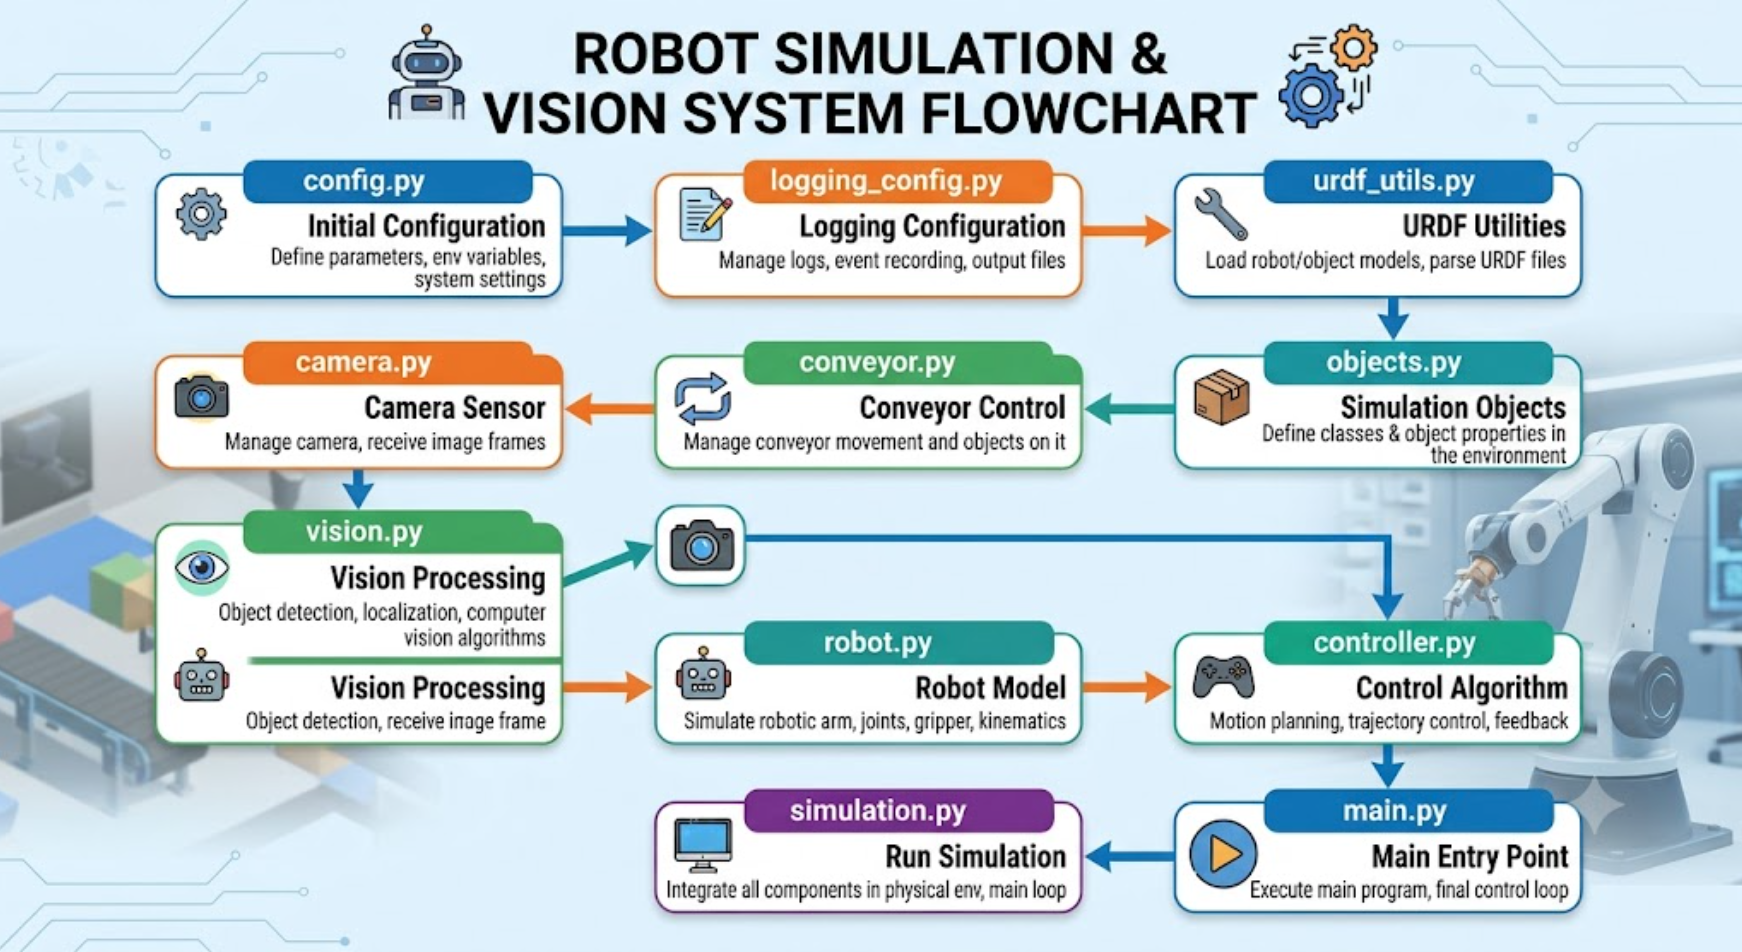
\includegraphics[width=0.85\textwidth]{img/fig33.png}
	\caption{Flowchart of simulation modules}
	\label{fig:fig33}
\end{figure}

\subsection{Simulation Section Documentation: The \texttt{config.py} Module}

\subsubsection{Module Overview}
The \texttt{config.py} module serves as the central configuration core for the Digital Twin simulation within the PyBullet environment. This file houses a static class named \texttt{Config}, which encapsulates all tunable constants pertaining to physical simulation, mechanical mechanisms, camera optical parameters, and the computer vision pipeline.

\subsubsection{Design Objectives}
The primary objective behind designing this module is to implement the "Single Source of Truth" architectural pattern for system parameters. In complex robotic and simulation systems, scattering hardcoded constants (magic numbers) across multiple source files degrades code readability and increases human error during fine-tuning. Consolidating all parameters into this single class enables calibration and global system behavior modification from a unified point.

\subsubsection{Role within the Overall System}
This module functions as the global regulator for the entire simulation pipeline. Parameters ranging from physics engine update frequencies to robot arm kinematic coordinates, camera focal properties, and decision thresholds in anomaly detection neural networks are explicitly dictated by this class to all downstream modules. This structure allows developers to configure various simulation scenarios without needing to alter or inspect the internal execution logic of other files.

\subsubsection{General Structure and Key Components}
The \texttt{Config} class is logically structured into several key sub-components:

\begin{itemize}
	\item Physics and Simulation Parameters (\texttt{Simulation}): Defines the graphical user interface (\texttt{GUI}) state, gravitational acceleration ($-9.81 \text{ m/s}^2$), the total simulation step limit (6000 steps for extended demonstration runs), and the simulation time step set to $1/240$ seconds—the standard PyBullet step size for accurate rigid-body dynamics calculation.
	
	\item Conveyor Belt Specifications (\texttt{Conveyor}): Specifies the geometric dimensions (length, width, height), the default motion velocity ($0.5 \text{ m/s}$), and its 3D spatial placement coordinates.
	
	\item Robotic Arm Coordinates (\texttt{Robot Arm}): Specifies the base mounting position of the robot alongside key operational waypoints, including the pick-up target point (\texttt{Pick}) and release targets for both repair (\texttt{Repair}) and scrap (\texttt{Scrap}) routing paths. These spatial coordinates serve as the baseline inputs for inverse kinematics calculations in the robot control module.
	
	\item Camera and Optics (\texttt{Camera}): Configures rendering parameters including spatial resolution ($320 \times 320$ pixels), field of view ($\text{FOV} = 35^\circ$), and near/far clipping planes. The camera's spatial position is strategically offset along the X-axis ($X = -1.5$) to ensure image acquisition and model inference complete prior to the component reaching the sorting decision gates.
	
	\item Object Spawning Dynamics (\texttt{Object Spawning}): Controls the temporal spawn interval between consecutive parts on the conveyor. Relative to the $240 \text{ Hz}$ update frequency, this interval is configured to 350 steps ($\approx 1.45 \text{ seconds}$), maintaining adequate physical separation between adjacent components.
	
	\item AI Vision Pipeline Parameters (\texttt{Vision Pipeline}): Specifies the interface between the simulator and trained models. It dictates file paths for YOLOv8 model weights (\texttt{best.pt}), anomaly detection model directories (\texttt{PatchCore/ResNet-18}), and downstream classification decision thresholds.
\end{itemize}


\subsubsection{Mode of Operation}
Because all variables are defined as static class attributes, these parameters are loaded statically into memory. Other modules can directly query their values either by accessing the class namespace (e.g., \texttt{Config.CONVEYOR\_SPEED\_DEFAULT}) or by instantiating the class.

In the AI vision pipeline, system evaluation is governed by two decision thresholds:

\begin{itemize}
	\item Anomaly Confidence Threshold (\texttt{ANOMALY\_CONFIDENCE\_THRESHOLD}): Set to $0.7$, meaning that if the output confidence score from the PatchCore model reaches or exceeds $70\%$, the component is routed to the defect surface area evaluation phase.
	
	\item Strategic Decision Threshold (\texttt{DEFECT\_AREA\_SCRAP\_THRESHOLD}): Set to $0.15$, indicating that if the defective surface area exceeds $15\%$ of the total component surface, a routing command is issued to direct the part to the scrap bin (\texttt{Scrap}); otherwise, the component is routed to the repair trajectory (\texttt{Repair}).
\end{itemize}

\subsubsection{Inter-Module Connectivity}
The \texttt{config.py} file maintains no external module import dependencies except for the standard \texttt{os} library for path resolution; however, it is imported across all secondary modules:

\begin{itemize}
	\item The \texttt{robot.py} and \texttt{conveyor.py} modules for accessing physical dimensions and kinematic coordinates.
	\item The \texttt{camera.py} module for obtaining projection matrices and rendering options.
	\item The \texttt{vision.py} module for loading neural network weights (such as the \texttt{best.pt} file trained in previous phases) and enforcing inference decision thresholds.
	\item The \texttt{main.py} and \texttt{simulation.py} modules for controlling the main simulation loop and object spawning schedules.
\end{itemize}

\subsubsection{Summary}
By establishing a centralized, modular architecture, the \texttt{config.py} module simplifies the management of complex operations in the Digital Twin simulator. Explicitly defining physical boundaries, kinematic waypoints, and deep learning inference thresholds within this single configuration file ensures high software engineering standards, allowing for parameter testing—such as varying conveyor speed or modifying defect sensitivity—without requiring code modifications across operational logic.

\subsection{Simulation Section Documentation: The \texttt{logging\_config.py} Module}

\subsubsection{Module Overview}
The \texttt{logging\_config.py} module configures a centralized logging framework across the Digital Twin simulation ecosystem. Upon importing this module, the fundamental logging configuration is initialized once in memory, exposing a shared logger instance for global project utilization.

\subsubsection{Design Objectives}
In complex robotics and engineering software development, using primitive stdout statements (e.g., \texttt{print}) for monitoring and debugging is insufficient, as they lack crucial metadata like timestamps, log severity levels, and structured file persistence capabilities. This module replaces unorganized output streams with a standardized, unified logging architecture, ensuring consistent and traceable output formatting across all program modules.

\subsubsection{Role within the Overall System}
This module operates as the diagnostic logging backbone of the simulator. It logs physical state events, precise camera frame capture timings, and computer vision inference outputs. This integrated monitoring capability provides developers with real-time, fine-grained visibility into system behavior during simulation runs.

\subsubsection{General Structure and Key Components}
Constructed using Python's standard \texttt{logging} library, the module comprises two core components:

\begin{itemize}
	\item Base Configuration (\texttt{logging.basicConfig}): Configures the logging threshold to \texttt{INFO}, capturing standard execution flow, warnings, and error events. Log formatting is explicitly set to \texttt{\%(asctime)s [\%(levelname)s] \%(message)s}, which appends precise execution timestamps, severity levels (e.g., \texttt{INFO} or \texttt{ERROR}), and the primary message body.
	
	\item Dedicated Namespace (\texttt{logging.getLogger}): Instantiates a logger object under the \texttt{"DigitalTwin"} namespace. Enforcing a distinct logger namespace guarantees that emitted logs remain isolated and easily identifiable when integrated with larger software stacks.
\end{itemize}

\subsubsection{Mode of Operation}
The module relies on Python's run-once execution pattern upon module import. When the first module in the project imports this file, \texttt{basicConfig} is executed to apply root-level logging formatting. Subsequently, the \texttt{logger} instance is created and exposed to the application. On secondary imports by other modules, the initial configuration is not re-executed; instead, the existing \texttt{logger} reference is returned—effectively implementing a Singleton design pattern.

\subsubsection{Inter-Module Connectivity}
Operating as an infrastructure module, this file has zero internal dependencies within the project, yet it is imported across almost all primary system components:

\begin{itemize}
	\item In the \texttt{vision.py} module: Logs image processing results, detected object classes, and associated confidence scores.
	\item In the \texttt{simulation.py} and \texttt{main.py} modules: Reports simulation lifecycle events, such as object spawning instances or system process initiation and termination.
	\item In the \texttt{camera.py} module: Tracks and logs frame capture status and optical rendering states.
\end{itemize}

\subsubsection{Summary}
Despite its minimal codebase, the \texttt{logging\_config.py} module adds substantial software engineering value to the simulation framework. By standardizing execution output streams, it streamlines real-time monitoring, debugging, and performance evaluation of AI models interacting with the physical environment, elevating software diagnostics to industrial-grade standards.

\subsection{Simulation Section Documentation: The \texttt{urdf\_utils.py} Module}

\subsubsection{Module Overview}
The \texttt{urdf\_utils.py} module serves as the procedural asset generation engine within the simulator. This file contains a suite of utility functions tasked with dynamically instantiating and saving standard 3D asset files—such as Unified Robot Description Format (\texttt{URDF}) and Wavefront \texttt{OBJ} files—to disk at runtime for immediate loading by the PyBullet physics engine.

\subsubsection{Design Objectives}
In robotics software development, relying on static external CAD or \texttt{URDF} files can introduce cross-platform portability challenges and file-path dependencies. The primary design goal of this module is to eliminate the need to distribute static external assets alongside the codebase. Through this programmatic approach, the system dynamically constructs its physical and environmental components using explicit parameters at runtime. Furthermore, this module addresses an inherent limitation in PyBullet regarding texture mapping by synthesizing a specialized geometric mesh file.

\subsubsection{Role within the Overall System}
This module functions as the programmatic asset factory for the physical and visual infrastructure of the simulation environment. Camera stands, robot end-effectors, sorting collection bins (\texttt{Repair/Scrap}), and visual planes holding component images are all instantiated through this module. Effectively, this file serves as the interface between software execution logic and the physics engine to define geometries, mass properties, friction coefficients, and kinematic structures for environmental objects.

\subsubsection{General Structure and Key Components}
The module comprises four core engineering functions:

\begin{itemize}
	\item \texttt{create\_camera\_stand\_urdf}: Generates the kinematic structure for the camera mounting stand.
	\item \texttt{create\_magnetic\_tool\_urdf}: Constructs the magnetic tool attachment mounted onto the robotic arm's end-effector.
	\item \texttt{create\_bucket}: Programmatically builds physical sorting bins directly via the PyBullet native API.
	\item \texttt{create\_textured\_plane\_obj}: Synthesizes a custom planar geometric mesh (\texttt{Mesh}) for high-fidelity image-to-surface texture mapping.
\end{itemize}

\subsubsection{Mode of Operation}
The operational logic of this module is divided into two mechanisms: XML/OBJ text file generation and direct multi-body physical object instantiation in the physics simulation.

\begin{itemize}
	\item Kinematic Modeling (\texttt{URDF} Generation): Functions dedicated to the camera stand and magnetic tool write XML structures describing hierarchical trees of links and joints. For example, in the camera stand assembly, four distinct links (\texttt{base}, \texttt{pole}, \texttt{arm}, and \texttt{camera\_body}) are joined using rigid connections (\texttt{type="fixed"}) to form a single rigid body. Setting the mass attribute to zero (\texttt{mass value="0"}) anchors the camera stand statically in the environment.
	
	\item Physical Bucket Instantiation: Rather than generating an external file, the \texttt{create\_bucket} function interfaces directly with low-level physics API calls. It programmatically constructs a base floor and four side walls into a unified multi-body (\texttt{MultiBody}). A subtle design choice in this geometry is the lowered front lip wall, which facilitates unimpeded component entry into the bin. Additionally, setting the base mass to zero (\texttt{baseMass=0}) prevents bin displacement upon impact with the robot or dropped parts, while a high lateral friction coefficient (\texttt{lateralFriction=0.8}) ensures physical stability for sorted components.
	
	\item Advanced UV Texture Mapping: The \texttt{create\_textured\_plane\_obj} function overcomes a key visual rendering limitation. In PyBullet, mapping images directly onto primitive geometries (such as \texttt{GEOM\_BOX}) causes the physics engine to tile or crop textures based on physical dimensions (in meters), introducing visual distortion or unwanted scaling. This function programmatically writes a standard \texttt{OBJ} file that explicitly maps UV coordinates normalized from $0$ to $1$ across the four vertices of a planar face. This guarantees that industrial dataset images render tangentially onto component surfaces without geometric distortion.
\end{itemize}

\subsubsection{Inter-Module Connectivity}
\begin{itemize}
	\item The \texttt{simulation.py} module calls these functions to instantiate the camera stand and sorting bins at spatial coordinates provided by \texttt{config.py}.
	\item The \texttt{robot.py} module relies on this file to generate and attach the magnetic tool as its end-effector.
	\item The \texttt{objects.py} (or \texttt{conveyor.py}) module utilizes the generated \texttt{OBJ} meshes to render visual component representations moving along the conveyor belt.
\end{itemize}

\subsubsection{Summary}
By combining programmatic procedural generation with automated 3D asset synthesis, the \texttt{urdf\_utils.py} module enhances simulation flexibility. Leveraged through a deep understanding of PyBullet's mass mechanics (for static anchoring) and texture mapping (via custom \texttt{OBJ} mesh synthesis), this module reduces redundant boilerplate code while guaranteeing high physical and visual fidelity for real-time computer vision inference within the Digital Twin environment.


\subsection{Simulation Section Documentation: The \texttt{objects.py} Module}

\subsubsection{Module Overview}
The \texttt{objects.py} module implements a comprehensive Object Lifecycle Management system within the simulation environment. This module is responsible for spawning, position tracking, state management, and the ultimate deletion of dynamic industrial components moving along the conveyor belt. Furthermore, a spatial checkpoint detection mechanism is embedded within this module to synchronize physical dynamics events with computer vision inference triggers.

\subsubsection{Design Objectives}
In rigid-body physics engines such as PyBullet, objects are identified merely through raw numerical IDs, lacking logical identities, class labels, or motion histories. The primary design objective of this module is to construct an abstraction layer that wraps these numerical IDs into meaningful software entities (\texttt{Tracked Objects}). This enables the high-level central controller to interact with conceptual entities—such as "part class," "current operational state," and "spatial events"—rather than interfacing directly with low-level physics API calls.

\subsubsection{Role within the Overall System}
This module functions as the scene manager and event monitor within the Digital Twin framework. From the instant an industrial component (e.g., a screw, nut, or transistor) is spawned on the conveyor belt according to the schedule, until it is picked up by the robotic arm or exits the workspace, its lifecycle remains entirely under the governance of this module. Its most critical role is emitting software events based on the spatial positions of components, ensuring the camera captures frames at the exact required time steps.

\subsubsection{General Structure and Key Components}
Utilizing an Object-Oriented Programming (OOP) design, this module consists of the following components:

\begin{itemize}
	\item \textbf{The \texttt{create\_dummy\_texture} Function:} An OpenCV-based utility tool that dynamically synthesizes placeholder textures featuring text labels and colored borders if actual component image files are missing. This function supports testing scenarios and mock vision debugging.
	\item \textbf{The \texttt{ObjectState} Class:} An enumeration (\texttt{Enum}) acting as a Finite State Machine (FSM) that dictates the four stages of a component's lifecycle: spawned (\texttt{SPAWNED}), moving along the conveyor (\texttt{ON\_CONVEYOR}), removed from the workspace (\texttt{REMOVED}), and dropped out of bounds (\texttt{FELL\_OFF}).
	\item \textbf{The \texttt{TrackedObject} Class:} A lightweight wrapper around the PyBullet body ID that binds essential metadata—such as object class (\texttt{obj\_type}) and string label (\texttt{label})—to the entity. It exposes properties that extract the real-time spatial position and orientation of the object directly from the physics engine.
	\item \textbf{The \texttt{ObjectManager} Class:} The central management engine containing active object dictionaries, checkpoint tracking lists, and object spawning counters.
\end{itemize}

\subsubsection{Mode of Operation}
The operational logic of the \texttt{ObjectManager} class revolves around three primary axes:

\begin{enumerate}
	\item \textbf{Smart Spawning (\texttt{spawn\_object}):} The \texttt{spawn\_object} method verifies image file existence prior to instantiation to prevent silent rendering failures (a fail-fast mechanism). The system then defines a primitive box for the collision shape while leveraging the custom \texttt{create\_textured\_plane\_obj} function (from the \texttt{urdf\_utils} module) for the visual shape. This dual-geometry strategy guarantees that texture mapping (\texttt{UV Mapping}) matches the exact aspect ratio and scale of the source image. Finally, lateral friction parameters are configured to prevent component slippage along the conveyor belt.
	
	\item \textbf{Tracking and Memory Garbage Collection:} The \texttt{update\_tracking} method is invoked on every iteration of the simulation loop. It evaluates the Z-axis height of tracked objects; if a component drops below $Z = -1.0$, the system flags it as out-of-bounds (\texttt{FELL\_OFF}) and automatically purges it from both the physics engine memory and internal tracking dictionaries to prevent resource leaks.
	
	\item \textbf{Spatial Event Triggering:} To maintain synchronization with the camera module, the system tracks virtual spatial checkpoints along the X-axis. Within \texttt{update\_tracking}, the previous spatial position (\texttt{last\_position}) is compared against the current position (\texttt{curr\_pos}). When an object crosses a predefined virtual line along the X-axis, a software event containing the object ID and station identifier is emitted to trigger downstream pipeline modules (such as computer vision inference).
\end{enumerate}

\subsubsection{Inter-Module Connectivity}
\begin{itemize}
	\item \textbf{The \texttt{urdf\_utils.py} Module:} Direct dependency on custom textured plane generation to project industrial component images onto planar surface meshes without visual distortion.
	\item \textbf{The \texttt{config.py} Module:} Supplies physical dimension parameters (planar thickness and base sizing) and component mass properties.
	\item \textbf{The \texttt{simulation.py} Module (Main Loop):} Continuously calls the \texttt{update\_tracking} method to receive system events and issue operational commands to camera and robotic subsystems.
\end{itemize}

\subsubsection{Summary}
By encapsulating PyBullet API complexities, the \texttt{objects.py} module transforms dynamic object management into a structured and predictable workflow. The inclusion of automated garbage collection for out-of-bounds objects and spatial checkpoint detection provides a robust bridge linking the physical dynamics of the Digital Twin with high-level AI decision logic.

\subsection{Simulation Section Documentation: The \texttt{conveyor.py} Module}

\subsubsection{Module Overview}
The \texttt{conveyor.py} module manages and controls the conveyor belt subsystem within the simulation environment. This file houses the \texttt{ConveyorController} class, which defines the physical properties and visual geometry of the belt while programmatically implementing the kinematics governing component motion along the line.

\subsubsection{Design Objectives}
In rigid-body physics engines like PyBullet, simulating a continuous, deformable surface (such as a real physical conveyor belt) using conventional mesh dynamics introduces severe computational overhead and physical instability. The primary design objective of this module is to bypass these constraints using an established robotics simulation technique: the conveyor belt is modeled as a static rigid body, and driving forces are transferred directly to contacting objects rather than driving belt dynamics. Furthermore, the ground plane ID (\texttt{ground\_id}) is explicitly passed to the system to eliminate hardcoded assumptions that default body ID zero to the floor plane.

\subsubsection{Role within the Overall System}
This module represents the primary transport mechanism within the simulation. The continuous throughput of components—from their initial spawning points to the camera frame view and onward to sorting collection stations (\texttt{Repair/Scrap})—relies on the execution of this module. The conveyor controller exposes interfaces allowing the central controller to halt, resume, or dynamically adjust belt speed during simulation runs.

\subsubsection{General Structure and Key Components}
The module's core logic is centered within the \texttt{ConveyorController} class, which includes the following components:

\begin{itemize}
	\item \textbf{Initialization and Body Instantiation (\texttt{\_create\_body}):} Generates a static box geometry with zero mass (disabling gravity response) and a high lateral friction coefficient ($1.0$) to prevent object slippage.
	\item \textbf{State Management Interface:} Exposes \texttt{start}, \texttt{stop}, \texttt{set\_speed}, and \texttt{get\_speed} API methods to control conveyor behavior across operational scenarios.
	\item \textbf{Physics Update Engine (\texttt{update\_physics}):} The primary kinematic method invoked during every physics execution step to monitor contact manifolds and apply directional velocity vectors.
\end{itemize}

\subsubsection{Mode of Operation}
The kinematic movement logic resides inside the \texttt{update\_physics} method, which executes at every simulation time step (typically $\frac{1}{240}$ seconds based on environment configuration). The execution pipeline operates as follows:

\begin{enumerate}
	\item \textbf{Contact Detection:} Manifold contact points between the conveyor geometry and environment bodies are queried via \texttt{p.getContactPoints}.
	\item \textbf{Smart Contact Filtering:} To prevent non-physical artifacts, contact manifolds are systematically filtered. Contacts involving the floor plane (\texttt{ground\_id}), penetration depths exceeding $0.005$ meters (\texttt{contact[8] > 0.005}), and contacts with static environment geometries (such as zero-mass camera stands or sorting bins) are discarded.
	\item \textbf{Direct Velocity Override:} For valid dynamic components resting on the belt surface (such as screws or transistors), the system reads their existing linear and angular velocities before overwriting the translational velocity vector. The linear velocity along the X-axis is explicitly forced to match the effective conveyor belt speed ($v_{\text{effective}}$), while Y-axis, Z-axis, and angular momentum ($ang\_vel$) components remain untouched:
	
	$$\vec{V}_{\text{target}} = [v_{\text{effective}}, v_y, v_z]$$
	
	This formulation drives the component forward along the belt path while preserving natural physical dynamics, such as minor surface rolling or settling.
\end{enumerate}

\subsubsection{Inter-Module Connectivity}
\begin{itemize}
	\item \textbf{The \texttt{config.py} Module:} Provides precise physical dimensions (length, width, height) and default belt transport speed parameters.
	\item \textbf{The \texttt{simulation.py} Module (Main Loop):} Calls the \texttt{update\_physics} method on every tick iteration to enforce continuous component transport.
	\item \textbf{The \texttt{objects.py} Module:} Components instantiated as tracked objects (\texttt{Tracked Objects}) are translated by this module's velocity field, advancing them across virtual spatial checkpoints.
\end{itemize}

\subsubsection{Summary}
The \texttt{conveyor.py} module demonstrates efficient design principles within industrial simulation environments. By utilizing direct velocity override methods on contacting bodies instead of executing complex multi-body mesh dynamics, this module achieves smooth, stable, and deterministic motion with minimal computational load in PyBullet. This kinematic stability serves as a crucial requirement for capturing sharp, motion-blur-free images across downstream vision processing pipelines.


\subsection{Simulation Section Documentation: The \texttt{camera.py} Module}

\subsubsection{Module Overview}
The \texttt{camera.py} module provides an abstraction layer for simulating the optical acquisition system within the Digital Twin environment. Modeling an overhead industrial camera mounted perpendicular to the conveyor line, this module converts rendered 3D frames from the PyBullet physics engine into structured NumPy arrays suitable for downstream image processing using OpenCV and deep learning inference frameworks.

\subsubsection{Design Objectives}
The primary design objective of this module is to construct a standardized interface between the 3D physics environment and the 2D computer vision pipeline. AI frameworks like YOLO require input data adhering to specific formats, dimensions, and color channels (e.g., OpenCV's native BGR layout). This module encapsulates lens parameters, 3D scene rendering calls, and matrix transformations into a unified interface, delivering standardized image arrays to the central system controller.

\subsubsection{Role within the Overall System}
This module functions as the primary optical sensor for the automated quality control system. The virtual camera is strategically positioned upstream of the sorting gates (\texttt{Repair/Scrap}) to capture frames as industrial components cross a virtual checkpoint. Output image matrices from this module serve as direct inputs to downstream object detection and anomaly localization neural networks.

\subsubsection{General Structure and Key Components}
The module's core logic is contained within the \texttt{CameraAPI} class, which encapsulates the following spatial and mathematical attributes:

\begin{itemize}
	\item \textbf{Spatial Coordinate Parameters:} Camera lens position (\texttt{eye\_position}) and target focal coordinates (\texttt{target\_position}).
	\item \textbf{View Matrix:} Specifies the position, orientation, and spatial direction of the camera in global 3D coordinates.
	\item \textbf{Projection Matrix:} Governs the 3D-to-2D projection mapping based on configured field-of-view (\text{FOV}) and frame aspect ratio settings.
	\item \textbf{Frame Acquisition Interface Methods:} The \texttt{get\_frame} method extracts RGB color channels, while \texttt{get\_depth} extracts corresponding depth maps.
\end{itemize}

\subsubsection{Mode of Operation}
The execution pipeline leverages standard computer graphics and image processing operations:

\begin{enumerate}
	\item \textbf{Geometric Calibration:} During system initialization, target focal coordinates are fetched from configuration files, and lens positions are computed by applying a vertical height offset (\texttt{CAMERA\_Z\_OFFSET}). The corresponding View and Projection matrices are constructed via PyBullet native API calls and cached in memory to eliminate redundant matrix recalculations during inference loops.
	
	\item \textbf{Adaptive Rendering Selection:} Frame acquisition methods dynamically select rendering backends based on display settings. When the graphical user interface (GUI) is enabled, hardware-accelerated OpenGL rendering (\texttt{ER\_BULLET\_HARDWARE\_OPENGL}) is utilized for execution speed; otherwise, lightweight software rendering (\texttt{ER\_TINY\_RENDERER}) is selected for headless execution.
	
	\item \textbf{Color Space Conversion:} The \texttt{get\_frame} method converts raw PyBullet RGBA buffers into standard image matrices. The raw 1D buffer is reshaped into a 3D array ($\text{Height} \times \text{Width} \times 4$), and the alpha transparency channel is discarded. Using \texttt{cv2.cvtColor}, the color space is converted from RGB to BGR format. This conversion ensures compatibility with OpenCV function calls and input layer conventions expected by pretrained YOLO architectures.
	
	\item \textbf{Depth Buffer Extraction:} The \texttt{get\_depth} method executes frame rendering to extract raw Z-buffer values (representing spatial distance to the lens array) as a 2D matrix. This depth map can support dimension estimation or spatial occlusion detection in expanded operational workflows.
\end{enumerate}

\subsubsection{Inter-Module Connectivity}
\begin{itemize}
	\item \textbf{The \texttt{config.py} Module:} Supplies optical parameter values, including spatial resolution ($320 \times 320$ pixels), field-of-view ($35^\circ$), near/far plane clipping bounds, and mounting spatial coordinates.
	\item \textbf{The \texttt{vision.py} Module:} Serves as the primary consumer of rendered frame output. BGR image matrices returned by \texttt{get\_frame} are passed directly into downstream anomaly detection workflows.
	\item \textbf{The \texttt{simulation.py} Module (Main Loop):} Acts as the execution coordinator, issuing frame acquisition calls when components cross spatial checkpoints.
	\end{itemize}
		
\subsubsection{Summary}
By implementing spatial camera calibration and color space transformations, the \texttt{camera.py} module ensures that synthetic visual data captured in simulation closely aligns with real-world industrial camera acquisition standards. Preserving fixed-perspective camera assumptions matches the training distribution of the vision models, supporting real-time inference execution across the Digital Twin pipeline.


\subsection{Simulation Section Documentation: The \texttt{vision.py} Module}

\subsubsection{Module Overview}
The \texttt{vision.py} module serves as the primary inference engine and decision-making pipeline within the Digital Twin framework. Responsible for analyzing raw input frames captured by the overhead camera system, it leverages deep learning architectures to evaluate the structural quality of moving industrial components. The module features two distinct implementations: a \texttt{MockVisionModule} designed for early-stage debugging and physical dynamics prototyping, and a production-grade \texttt{RealVisionModule} incorporating a two-stage inspection pipeline that pairs a YOLOv8 object detector with PatchCore anomaly localization models.

\subsubsection{Design Objectives}
The primary objective of this module is enforcing a strict separation of concerns between computer vision processing logic and physics engine dynamics. Neural network inference introduces non-negligible computational overhead; therefore, the module incorporates aggressive model preloading, memory caching, and selective region-of-interest cropping to mitigate frame drops in the main PyBullet loop. The two-stage pipeline architecture—combining dynamic bounding box detection with targeted anomaly mask generation—ensures that computational resources for dense surface inspection (e.g., via PatchCore) are restricted to localized target regions rather than processing full-frame camera arrays.

\subsubsection{Role within the Overall System}
This module performs the role of the automated quality control inspector across the digital conveyor line. As components cross the active optical checkpoint, the module processes the acquired frame and generates a discrete classification decision: \texttt{GOOD} (nominal component), \texttt{REPAIR} (reworkable defect), or \texttt{SCRAP} (unrecoverable damage). This command is passed downstream to the robotic arm trajectory manager to direct component sorting routing.

\subsubsection{General Structure and Key Components}
The module's architecture is structured around three primary components:

\begin{itemize}
	\item \textbf{The \texttt{VisionClass} Enumeration:} An \texttt{Enum} standardizing output operational categories ($0$ for nominal \texttt{GOOD}, $1$ for reworkable \texttt{REPAIR}, and $2$ for unrecoverable \texttt{SCRAP}).
	\item \textbf{The \texttt{MockVisionModule} Class:} A testing harness generating deterministic or pseudo-random inspection results (controlled via fixed seeds) without loading heavy deep learning framework dependencies.
	\item \textbf{The \texttt{RealVisionModule} Class:} The primary AI processing engine, providing methods for VRAM memory allocation, weight preloading, YOLO object localization, Anomalib/PatchCore defect mask extraction, and decision tree evaluation.
\end{itemize}

\subsubsection{Mode of Operation}
The operational pipeline of the \texttt{RealVisionModule} executes through the following steps:

\begin{enumerate}
	\item \textbf{Hardware Allocation and Model Preloading:} During module initialization, the system verifies GPU acceleration availability (CUDA). The \texttt{preload\_all\_models} method transfers both the object detection network weights (\texttt{best.pt}) and class-specific anomaly inference engines (\texttt{PatchCore/ResNet}) into active GPU memory (VRAM), preventing I/O latency during real-time execution.
	
	\item \textbf{Region-of-Interest Localization (YOLO Cropping):} Upon frame capture, \texttt{\_detect\_and\_crop} passes the image array to the YOLO detector to locate component bounding boxes. Safety margins (\texttt{Crop Padding}) are applied to extracted bounding box coordinates to ensure peripheral surface defects along component boundaries are preserved during cropping.
	
	\item \textbf{Anomaly Map Generation and Contour Analysis:} The cropped bounding box is evaluated via a \texttt{TorchInferencer} engine, producing a global anomaly score alongside a binary spatial prediction mask. The \texttt{\_extract\_defect\_contours} method converts this spatial mask into localized contours, calculating the ratio of damaged surface pixels relative to overall component area. Local defect coordinates are subsequently translated back to global frame space by adding bounding box offsets.
	
	\item \textbf{Decision Logic:} The \texttt{\_score\_to\_class} method evaluates defect metrics against predefined quality assurance bounds:
	\begin{itemize}
		\item If the computed anomaly score remains below \texttt{ANOMALY\_CONFIDENCE\_THRESHOLD}, the component is classified as \texttt{GOOD}.
		\item When surface anomalies are detected, if the localized defect area ratio exceeds \texttt{DEFECT\_AREA\_SCRAP\_THRESHOLD} (e.g., $15\%$), a \texttt{SCRAP} classification is triggered. Otherwise, the component is assigned to \texttt{REPAIR}.
	\end{itemize}
	
	\item \textbf{Fail-Safe Fallback Handling:} The primary entry method (\texttt{infer}) incorporates exception-handling protocols. If input frames are dropped, YOLO detects no targets, or a class-specific anomaly model is missing, the system catches the exception, logs a warning, and defaults the component state to a nominal \texttt{GOOD} classification to prevent conveyor flow halts.
\end{enumerate}

\subsubsection{Inter-Module Connectivity}
\begin{itemize}
	\item \textbf{The \texttt{config.py} Module:} Supplies detection thresholds, model weight file paths (\texttt{.pt}), target class enumerations, and bounding box padding margins.
	\item \textbf{The \texttt{logging\_config.py} Module:} Logs real-time inspection records, including detected object categories, YOLO detection confidence, PatchCore anomaly scores, and defect area ratios.
	\item \textbf{The \texttt{camera.py} Module:} Serves as the input data source, providing rendered BGR image matrices.
	\item \textbf{The \texttt{simulation.py} Module (Main Loop):} Invokes the \texttt{infer} method as dynamic objects pass spatial optical checkpoints.
\end{itemize}

\subsubsection{Summary}
By combining a two-stage computer vision architecture with optimized inference execution, the \texttt{vision.py} module maintains real-time throughput while executing surface anomaly localization. Built-in model weight caching, coordinate normalization, and fail-safe exception handling convert raw visual input into deterministic control signals for downstream robotic sorting operations.


\subsection{Simulation Section Documentation: The \texttt{robot.py} Module}

\subsubsection{Module Overview}
The \texttt{robot.py} module implements the motion control architecture and operational logic for the industrial robotic manipulator (Franka Panda) within the simulation environment. This module translates high-level task commands—such as picking an inspected part and transferring it to a sorting bin—into continuous spatial trajectories and joint kinematics calculations.

\subsubsection{Design Objectives}
In industrial robotics simulation, path planning and dynamic grasping represent significant computational challenges. Modeling frictional grasp mechanics (friction cones) between finger pads and dynamic objects in rigid-body engines like PyBullet often induces physical jitter and instability. The primary design objective of this module is to abstract joint kinematic complexities and bypass physical contact limitations by employing a constraint-based magnetic gripping mechanism combined with a Finite State Machine (FSM) controller.

\subsubsection{Role within the Overall System}
This module functions as the primary physical actuator within the Digital Twin ecosystem. Upon receiving a quality inspection decision (\texttt{GOOD}, \texttt{REPAIR}, or \texttt{SCRAP}) from the \texttt{vision.py} module, the central controller dispatches target coordinates and routing basket vectors to this controller. As the final link in the automation loop, the robot picks designated components from the moving conveyor and deposits them into target destination locations.

\subsubsection{General Structure and Key Components}
The module's architecture is divided into two primary components:

\begin{itemize}
	\item \textbf{The \texttt{RobotState} Enumeration:} An \texttt{Enum} defining the state space of the robot's Finite State Machine (FSM) across nine distinct execution phases. These states include standby (\texttt{IDLE}), approach, grasp, lift, transfer, release, and home trajectory return.
	\item \textbf{The \texttt{RobotController} Class:} The primary control node handling Unified Robot Description Format (\texttt{URDF}) file loading, joint-level Proportional-Derivative (\texttt{PD}) controller configuration, Inverse Kinematics (\texttt{IK}) resolution, and end-effector tool management.
\end{itemize}

\subsubsection{Mode of Operation}
The module operates through a combination of spatial kinematics and state control logic, executed via the \texttt{step} method on each simulation frame:

\begin{enumerate}
	\item \textbf{Inverse Kinematics Resolution:} The \texttt{move\_ik} method translates target Cartesian coordinates $(X, Y, Z)$ into corresponding joint configurations $\theta_i$. Utilizing PyBullet's internal solver (\texttt{p.calculateInverseKinematics}), the function computes joint angle targets and applies joint torques via position control modes (\texttt{POSITION\_CONTROL}).
	
	\item \textbf{Dynamic Target Tracking:} A critical kinematic feature is implemented within the \texttt{MOVE\_TO\_PICK} and \texttt{GRASP} states. Because components advance along the active conveyor belt, the target position is non-static. On every simulation step, the real-time position of the target object (\texttt{target\_obj\_id}) is queried to update Cartesian targets (\texttt{target\_pos}), dynamically adapting the end-effector trajectory to match conveyor motion.
	
	\item \textbf{Timing and Delays:} Internal state timers (\texttt{state\_step}) govern FSM transitions. State transitions execute only after predefined step counts elapse (e.g., $120$ steps for approach trajectories, $60$ steps for grasp execution), ensuring joint control convergence to target waypoints.
	
	\item \textbf{Constraint-Based Grasping Dynamics:} Within the \texttt{GRASP} state, the physical finger closure is augmented by instantiating a rigid fixed constraint (\texttt{JOINT\_FIXED}). The system computes the relative transformation matrix between the end-effector tool frame and the target object frame. Inverting the tool transform and multiplying by the target object matrix yields:
	
	$$T_{\text{rel}} = T_{\text{tool}}^{-1} \times T_{\text{obj}}$$
	
	This yields the precise relative spatial orientation (\texttt{rel\_orn}). A fixed joint constraint is then instantiated between the end-effector and the target object, ensuring zero-slip transport. During the \texttt{RELEASE} state, this constraint is removed, allowing the object to fall into the designated bin under gravitational acceleration.
\end{enumerate}

\subsubsection{Inter-Module Connectivity}
\begin{itemize}
	\item \textbf{The \texttt{config.py} Module:} Supplies robot base placement coordinates (\texttt{ROBOT\_BASE\_POS}) and sorting destination target vectors (\texttt{Repair/Scrap Drop Positions}).
	\item \textbf{The \texttt{urdf\_utils.py} Module:} Dependency for invoking \texttt{create\_magnetic\_tool\_urdf} to construct custom end-effector URDF models.
	\item \textbf{The \texttt{simulation.py} Module (Main Loop):} Dispatches task assignments to the robot via the \texttt{dispatch} interface and executes the \texttt{step} update method within the primary physics loop.
\end{itemize}

\subsubsection{Summary}
By combining a Finite State Machine (FSM) architecture with Inverse Kinematics resolution, the \texttt{robot.py} module maintains synchronization between dynamic conveyor flows and robotic manipulation tasks. Replacing complex contact friction modeling with spatial joint constraints ensures physical stability across sorting routines within the Digital Twin environment.


\subsection{Simulation Section Documentation: The \texttt{controller.py} Module}

\subsubsection{Module Overview}
The \texttt{controller.py} module serves as the central coordinator and computational backbone of the Digital Twin simulator. It encapsulates the high-level decision-making logic of the entire system, seamlessly integrating spatial events along the conveyor belt, deep learning vision inference pipelines, and kinematic control directives for the robotic arm.

\subsubsection{Design Objectives}
In industrial automation systems, decoupling operational components represents a core principle of software engineering. Camera, computer vision, and robotic control submodules should not maintain direct tight coupling with one another. The primary design objective of this class is to implement a Mediator architectural pattern to maintain centralized flow control over system data streams. This architecture guarantees that asynchronous operational delays—such as deep learning inference latency or physical manipulator execution times—do not introduce physics instabilities or lead to dropped components along the transport line.

\subsubsection{Role within the Overall System}
This module functions as the supervisory control node across the simulator. All secondary functional modules operate as sub-nodes under its orchestration. Its primary responsibility includes continuous spatial checkpoint tracking, evaluating computer vision inference results, and converting quality decisions into physical hardware actuation (e.g., triggering conveyor halts and dispatching the robotic arm).

\subsubsection{General Structure and Key Components}
The \texttt{CentralController} class constitutes the primary body of this module, housing the following key components:

\begin{itemize}
	\item \textbf{State Management Trackers:} The \texttt{decisions} dictionary caches deep learning inference results to prevent redundant processing of passing components, while the \texttt{dispatched} set registers items for which robotic pick operations have already been triggered.
	\item \textbf{Operational Zone Definitions:} Establishes two critical virtual spatial regions: the camera capture inspection zone (\texttt{Camera\_Zone}) and the robotic picking zone (\texttt{Robot\_Pick\_Zone}).
	\item \textbf{Frame Acquisition and Visualization Engine (\texttt{\_capture\_and\_infer}):} Manages optical frame acquisition, dispatches image buffers to vision models, and handles real-time graphical overlay rendering on the user interface.
	\item \textbf{Event Handling Engine (\texttt{process\_events} and \texttt{update\_robot}):} Vital operational loops responsible for synchronizing physical line dynamics with higher-level robotic sorting logic.
\end{itemize}

\subsubsection{Mode of Operation}
The central controller functions via an event-driven architecture, executing along the following pipeline:

\begin{enumerate}
	\item \textbf{Camera Inspection Zone Management:}
	When the object management module (\texttt{objects.py}) flags a component crossing the virtual optical threshold, the controller invokes the \texttt{\_capture\_and\_infer} method. Upon receiving the rendered camera frame and passing it to the \texttt{vision} module, detected features are graphically rendered via OpenCV interface calls:
	\begin{itemize}
		\item The bounding box detected by the YOLO detector is drawn in green (indicating an identified target component).
		\item Anomaly contours generated by PatchCore models are mapped in red onto the localized region of interest, alongside the computed percentage of damaged surface area. This graphical representation is displayed to operators in a real-time window (\texttt{cv2.imshow}), while the final classification output is cached inside the \texttt{decisions} dictionary.
	\end{itemize}
	
	\item \textbf{Pick Zone Management and Line Synchronization:}
	When a component reaches the downstream picking threshold, the controller queries its cached decision state.
	\begin{itemize}
		\item If the component is classified as \texttt{GOOD}, no picking sequence is initiated, allowing the part to advance smoothly along the conveyor belt.
		\item If the component is flagged as defective (\texttt{REPAIR} or \texttt{SCRAP}), the controller immediately dispatches the robotic arm with spatial vectors mapped to the corresponding sorting bin.
		\item \textbf{Critical Line Synchronization:} Simultaneously, the controller issues an absolute motion halt command to the conveyor belt (\texttt{conveyor.set\_speed(0.0)}) to prevent the target part from moving out of reach or overshooting the line end.
	\end{itemize}
	
	\item \textbf{Line Resumption Protocol:}
	On every simulation tick, the \texttt{update\_robot} method advances the robot's state machine. Once the robotic arm completes its pick-and-place sequence and returns to its standby configuration (\texttt{RobotState.IDLE}), the controller issues a command to resume conveyor belt velocity (\texttt{CONVEYOR\_SPEED\_DEFAULT}).
\end{enumerate}

\subsubsection{Inter-Module Connectivity}
This module serves as the primary integration point across all system components:

\begin{itemize}
	\item \textbf{Object Manager (\texttt{object\_manager}):} Generates spatial position events.
	\item \textbf{Camera Subsystem (\texttt{camera}):} Delivers raw optical image arrays.
	\item \textbf{Vision Module (\texttt{vision\_module}):} Processes visual data and returns categorical quality assessments.
	\item \textbf{Robotic Controller (\texttt{robot}):} Receives kinematic dispatch trajectory commands (\texttt{dispatch}) targeting specified components.
	\item \textbf{Conveyor Controller (\texttt{conveyor}):} Receives dynamic velocity adjustments to stop and start the belt in sync with robotic state transitions.
\end{itemize}

\subsubsection{Summary}
By implementing a synchronized stop-and-go conveyor control mechanism in tandem with robotic manipulation, the \texttt{controller.py} module provides a robust, industrial-grade simulation interface. Caching inference results eliminates redundant processing overhead, while the real-time OpenCV graphical overlays provide transparent visualization of neural network layer outputs, delivering an integrated supervision system built on clean software architecture principles.



\subsection{Simulation Section Documentation: The \texttt{simulation.py} Module}

\subsubsection{Module Overview}
The \texttt{simulation.py} module serves as the orchestrator and lifecycle owner of the Digital Twin framework. Encapsulated within the \texttt{SimulationManager} class, it manages connection interfaces with the underlying PyBullet physics engine, loads static scene geometry, instantiates subsystem components, and drives the main simulation loop.

\subsubsection{Design Objectives}
In complex simulation architectures integrating multiple autonomous modules (including physics dynamics, vision inference pipelines, manipulator kinematics, and supervisory control nodes), the lack of a centralized lifecycle manager risks resource contention, memory leaks, and frame rate desynchronization. This module establishes a single entry and exit point for system execution. Furthermore, enforcing a Singleton design pattern guarantees that only a single simulator instance and active PyBullet physics client persist in memory at any given point during execution.

\subsubsection{Role within the Overall System}
This module functions as the operational core of the simulation platform. Subsystem modules (such as robotic controllers, optical cameras, and conveyor belts) do not execute independently; they are instantiated, registered in memory, and updated per time step through this module. Effectively, this file serves as the core integration bridge linking PyBullet physics computations with high-level software control logic.

\subsubsection{General Structure and Key Components}
The architecture of the \texttt{SimulationManager} class consists of the following key components:

\begin{itemize}
	\item \textbf{The Singleton Magic Method (\texttt{\_\_new\_\_}):} Enforces the Singleton pattern, preventing duplicate instantiations of the manager class.
	\item \textbf{Lifecycle Management Methods:} Includes \texttt{start} (initialization and physics engine connection), \texttt{disconnect} (graceful resource teardown and window closure), \texttt{stop} (execution pausing), and \texttt{reset} (resetting environment state to initial conditions).
	\item \textbf{Environment Loader (\texttt{load\_environment}):} Orchestrates the instantiation of physical assets (ground plane, conveyor assembly, camera mounting stand, robotic manipulator, and sorting bins) and initializes their respective controllers.
	\item \textbf{Main Simulation Loop Step (\texttt{step}):} Serves as the central execution loop, advancing physics time by discrete steps and triggering synchronous updates across all registered subsystems.
\end{itemize}

\subsubsection{Mode of Operation}
The module coordinates continuous execution through structured temporal sequencing:

\begin{enumerate}
	\item \textbf{Initialization and Dependency Injection:}
	Upon invoking the \texttt{start} method, the system determines the display mode (graphical interface via \texttt{GUI} or headless execution via \texttt{DIRECT}). It configures PyBullet asset paths and sets physics integration time steps. Within \texttt{load\_environment}, the module operates as an inversion-of-control container, injecting instantiated robot, camera, conveyor, and vision (\texttt{Mock} or \texttt{Real}) modules into the \texttt{CentralController} instance to establish inter-system connectivity.
	
	\item \textbf{Physics Integration Loop:}
	The \texttt{step} method, executed iteratively within the main program loop, enforces a structured sequence on every tick:
	\begin{itemize}
		\item Verifies active connection status with the physics server to prevent abrupt termination exceptions.
		\item Calls \texttt{update\_physics} on the conveyor module to apply linear friction vectors to resting components.
		\item Invokes the low-level \texttt{p.stepSimulation} API call, triggering PyBullet rigid-body dynamics and collision response solvers.
		\item Updates the spatial object tracking system (\texttt{object\_manager}) to detect spatial checkpoint crossings and generate event triggers.
		\item Passes spatial events to the supervisory controller (\texttt{controller.process\_events}) to synchronize computer vision inference and robotic actuation.
	\end{itemize}
	
	\item \textbf{Visual Stream Pacing and Pacing Control:}
	To minimize UI rendering overhead, live optical camera feeds are updated periodically every $N$ physics steps (configured via system parameters). Finally, when running in \texttt{GUI} display mode, execution speed is calibrated against real-time clocks using \texttt{time.sleep}, ensuring visual rendering aligns with human-perceivable speeds.
\end{enumerate}

\subsubsection{Inter-Module Connectivity}
This module occupies the root of the project's dependency graph, importing and orchestrating all functional submodules:

\begin{itemize}
	\item The \texttt{urdf\_utils} module for generating static geometric meshes and URDF assets.
	\item The \texttt{conveyor}, \texttt{robot}, \texttt{camera}, \texttt{vision}, and \texttt{objects} modules for constructing and initializing operational subsystems.
	\item The \texttt{controller} module for managing high-level orchestration logic across these subsystems.
	\item The \texttt{config} module for acquiring system runtime configuration parameters (including GUI modes, gravity vectors, and time-step values).
\end{itemize}

\subsubsection{Summary}
By combining Singleton lifecycle management with resource handling, the \texttt{simulation.py} module maintains stability across the Digital Twin execution loop. The design delegates domain-specific workloads (such as computer vision processing or kinematic inverse modeling) to specialized child modules, providing clean orchestration and supporting long-term system maintainability and scalability.

\subsection{Simulation Section Documentation: The \texttt{main.py} Execution Script}

\subsubsection{Script Overview}
The \texttt{main.py} script serves as the primary entry point and runtime environment for the Digital Twin simulation platform. This executable integrates all core modules—including system configurations, spatial object tracking, physics engine management, deep learning vision pipelines, and kinematic robotic controllers—managing the complete simulation lifecycle from initial part spawning to conveyor discharge.

\subsubsection{Design Objectives}
The primary objective of this module is establishing a fully isolated and managed execution environment. Complex simulation platforms interacting with temporary file I/O, VRAM memory allocations, and low-level physics engines (such as PyBullet) require strict resource management to prevent system deadlocks or memory leaks during unhandled exceptions. By employing robust exception handling blocks (\texttt{try-except-finally}) and automated resource teardown routines, this script ensures stability across varying execution environments.

\subsubsection{Execution Flow and Simulation Lifecycle}
The operational pipeline follows a structured sequence:

\begin{enumerate}
	\item \textbf{Environment Initialization:}
	Upon startup, console I/O encoding is explicitly forced to \texttt{UTF-8} to prevent runtime crashes during string formatting (such as Persian logging outputs). System environment variables are simultaneously configured to ensure safe third-party library execution.
	
	\item \textbf{Asset Management and Vision Execution Modes:}
	Based on the configured runtime setting (\texttt{VISION\_MODE}), execution branches into two distinct operational modes:
	\begin{itemize}
		\item \textbf{Production Mode (\texttt{real}):} The system queries the active \texttt{data} directory to load target industrial component dataset images (screws, nuts, transistors, etc.). Irrelevant files (such as ground-truth annotation masks) are filtered out, ensuring valid data streams enter downstream YOLO and PatchCore pipelines.
		\item \textbf{Test Scenario Mode (\texttt{scenario}):} For isolated debugging of mechanics and manipulator kinematics, the system uses the \texttt{create\_dummy\_texture} utility to synthesize temporary placeholder textures and files, simulating nominal (\texttt{GOOD}), reworkable (\texttt{REPAIR}), and unrecoverable (\texttt{SCRAP}) defect profiles.
	\end{itemize}
	
	\item \textbf{Dynamic Component Spawning:}
	To replicate realistic production line dynamics, components are instantiated sequentially rather than loaded simultaneously. An automated interval timer (\texttt{SPAWN\_INTERVAL}) releases items at fixed temporal offsets at the conveyor origin ($[-3.5, 0]$), preventing physical overlap errors within PyBullet collision solvers.
	
	\item \textbf{Main Simulation Loop and Termination Protocol:}
	The primary simulation loop advances time steps through continuous \texttt{sim.step()} execution. The script tracks component states until all spawned assets traverse the line and exit bounds (\texttt{FELL\_OFF}), triggering an automated graceful termination.
\end{enumerate}

\subsubsection{Exception Handling and Resource Teardown}
To maintain software engineering standards, the \texttt{finally} block guarantees critical cleanup operations upon execution termination:

\begin{itemize}
	\item Regardless of whether execution completes normally, is interrupted by the user (\texttt{KeyboardInterrupt}), or encounters a runtime exception, the connection to the PyBullet physics server is closed safely via \texttt{sim.disconnect()}.
	\item All temporary image textures and synthetic mesh files generated during \texttt{scenario} testing mode are removed from disk, preventing workspace pollution and storage leaks.
\end{itemize}

\subsubsection*{Summary of Simulation Documentation}
With the completion of technical documentation across \texttt{vision.py}, \texttt{robot.py}, \texttt{controller.py}, \texttt{simulation.py}, and \texttt{main.py}, all software components of this Digital Twin platform have been detailed. This documentation suite outlines the underlying object-oriented architecture, modular design, and integration methodologies connecting computer vision pipelines with physical robotics execution.

\section{Performance Evaluation and Execution Results}

\subsection{System Initialization}
Based on execution logs captured during the launcher script (\texttt{main.py}) run, the platform established a stable connection with the PyBullet physics server and initialized an OpenGL3 graphical interface (GUI). Upon detecting GPU acceleration support (\texttt{Device: cuda}), the \texttt{RealVision} module initiated the preloading sequence for all active neural models. During this phase, weights for the YOLOv8 object detector (\texttt{best.pt}) alongside six independent PatchCore anomaly detection models—corresponding to target component categories (screws, nuts, transistors, cables, bottles, and toothbrushes)—were transferred and cached within VRAM.

\subsection{Inference Pipeline Analysis}
During execution under \texttt{VISION\_MODE = 'real'}, six industrial components were dynamically spawned onto the moving conveyor belt. System inspection and classification results for these test items yielded the following:

\begin{itemize}
	\item \textbf{Nominal Components (\texttt{GOOD}):} Items such as \texttt{object\_001} (bottle), \texttt{object\_003} (transistor), and \texttt{object\_004} (cable) recorded low overall anomaly scores ($0.583$, $0.522$, and $0.586$, respectively). No defect surface area was detected for these components; consequently, they were assigned a \texttt{GOOD} classification label and allowed to pass through without interrupting conveyor flow.
	
	\item \textbf{Unrecoverable Scrap Components (\texttt{SCRAP}):} As evidenced in system logs and Figure~\ref{fig:fig31}, \texttt{object\_002} was identified as a metal nut (\texttt{metal\_nut}) by the YOLO detector with $89\%$ prediction confidence. The PatchCore inferencer computed a defect area ratio of \textbf{$24.25\%$} ($24.3\%$ on the UI display). Because this value exceeded the scrap threshold, the item was classified as \texttt{SCRAP}, dispatching the robotic manipulator to collect and deposit it into the designated red bin.
	
	\item \textbf{Reworkable Components (\texttt{REPAIR}):} Component \texttt{object\_005} (screw with a $3.70\%$ defect area) and \texttt{object\_006} (toothbrush) were routed to the repair pipeline. As shown in Figure~\ref{fig:fig32}, the toothbrush was detected with $78\%$ confidence, with defective surface areas ($11.36\%$ raw score, $11.4\%$ UI display) highlighted via red contour overlays. These items were collected by the manipulator and routed to the yellow repair station bin.
\end{itemize}

\subsection{Cyber-Physical Synchronization}
Execution logs demonstrate that the event-driven architecture and synchronization routines within the central supervisory controller (\texttt{controller.py}) operated as designed. The stop-and-go conveyor synchronization loop executed through the following recorded steps:

\begin{enumerate}
	\item Robotic motion dispatch command issued toward defective component target coordinates.
	\item Conveyor velocity throttled to zero (\texttt{[Conveyor] Speed set to: 0.0 m/s}).
	\item Task sequence completion and manipulator state return (\texttt{Robot returned to IDLE}).
	\item Conveyor transport resumption (\texttt{[Conveyor] Speed set to: 0.5 m/s}).
\end{enumerate}

\subsection{Live Monitoring User Interface}
Figures~\ref{fig:fig32} and~\ref{fig:fig31} confirm the performance of the visual monitoring interface. While PyBullet manages physical rigid-body dynamics and sensor updates, two secondary OpenCV rendering windows display live optical camera feeds and processed inference outputs. Overlaying green bounding boxes (YOLO localization) alongside red anomaly contours (PatchCore segmentation) and numerical defect area ratios delivers an intuitive visual interface for human operators.

\begin{figure}[H]
	\centering
	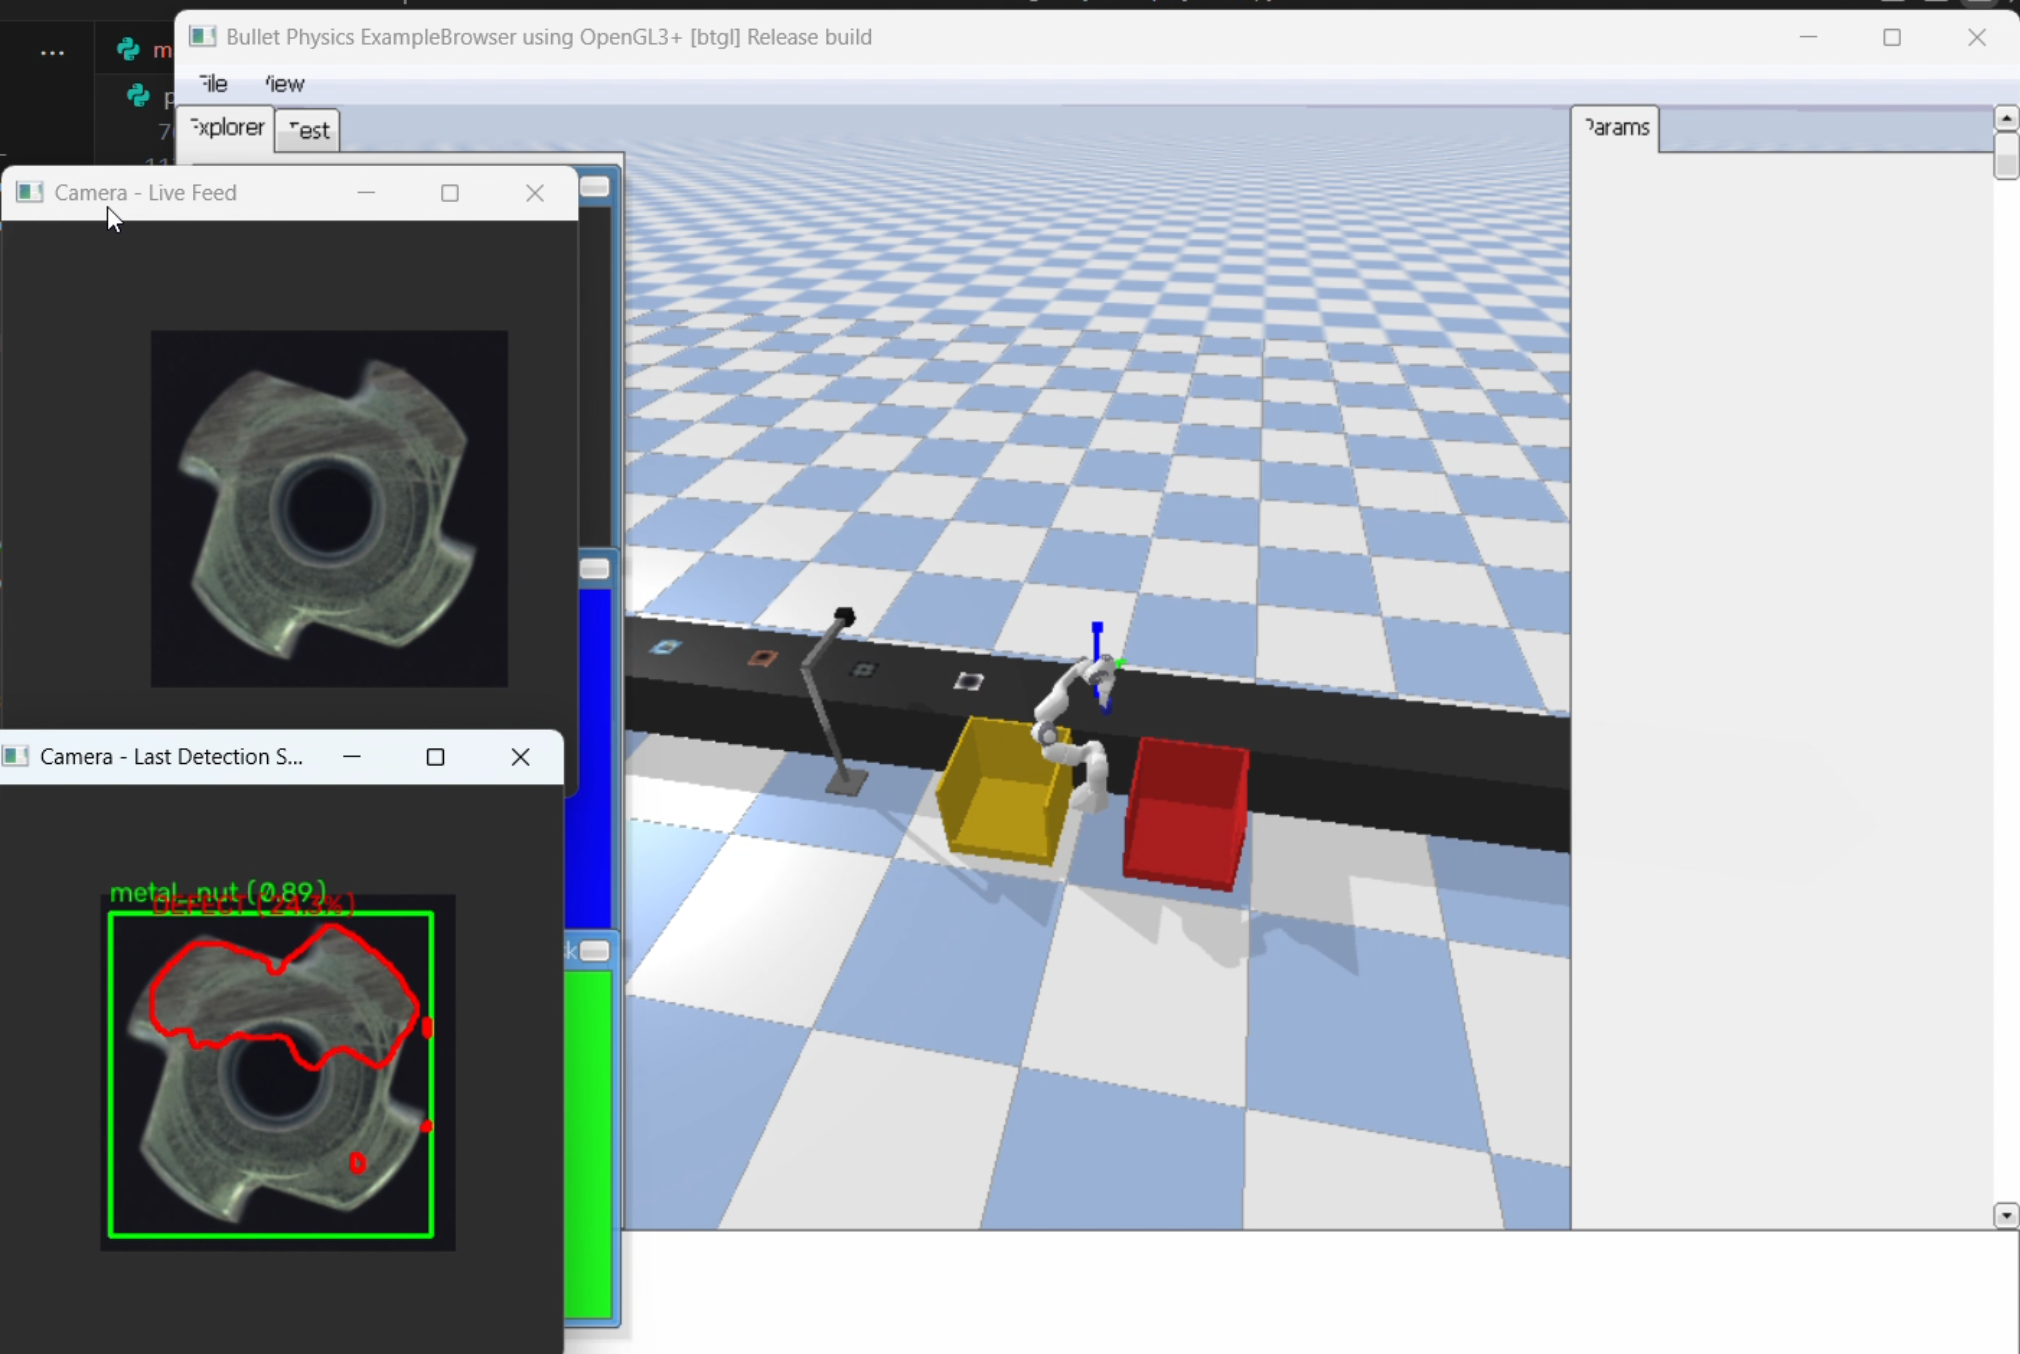
\includegraphics[width=0.85\textwidth]{img/fig31.png}
	\caption{Graphical simulation output and live visual monitoring display.}
	\label{fig:fig31}
\end{figure}

\begin{figure}[H]
	\centering
	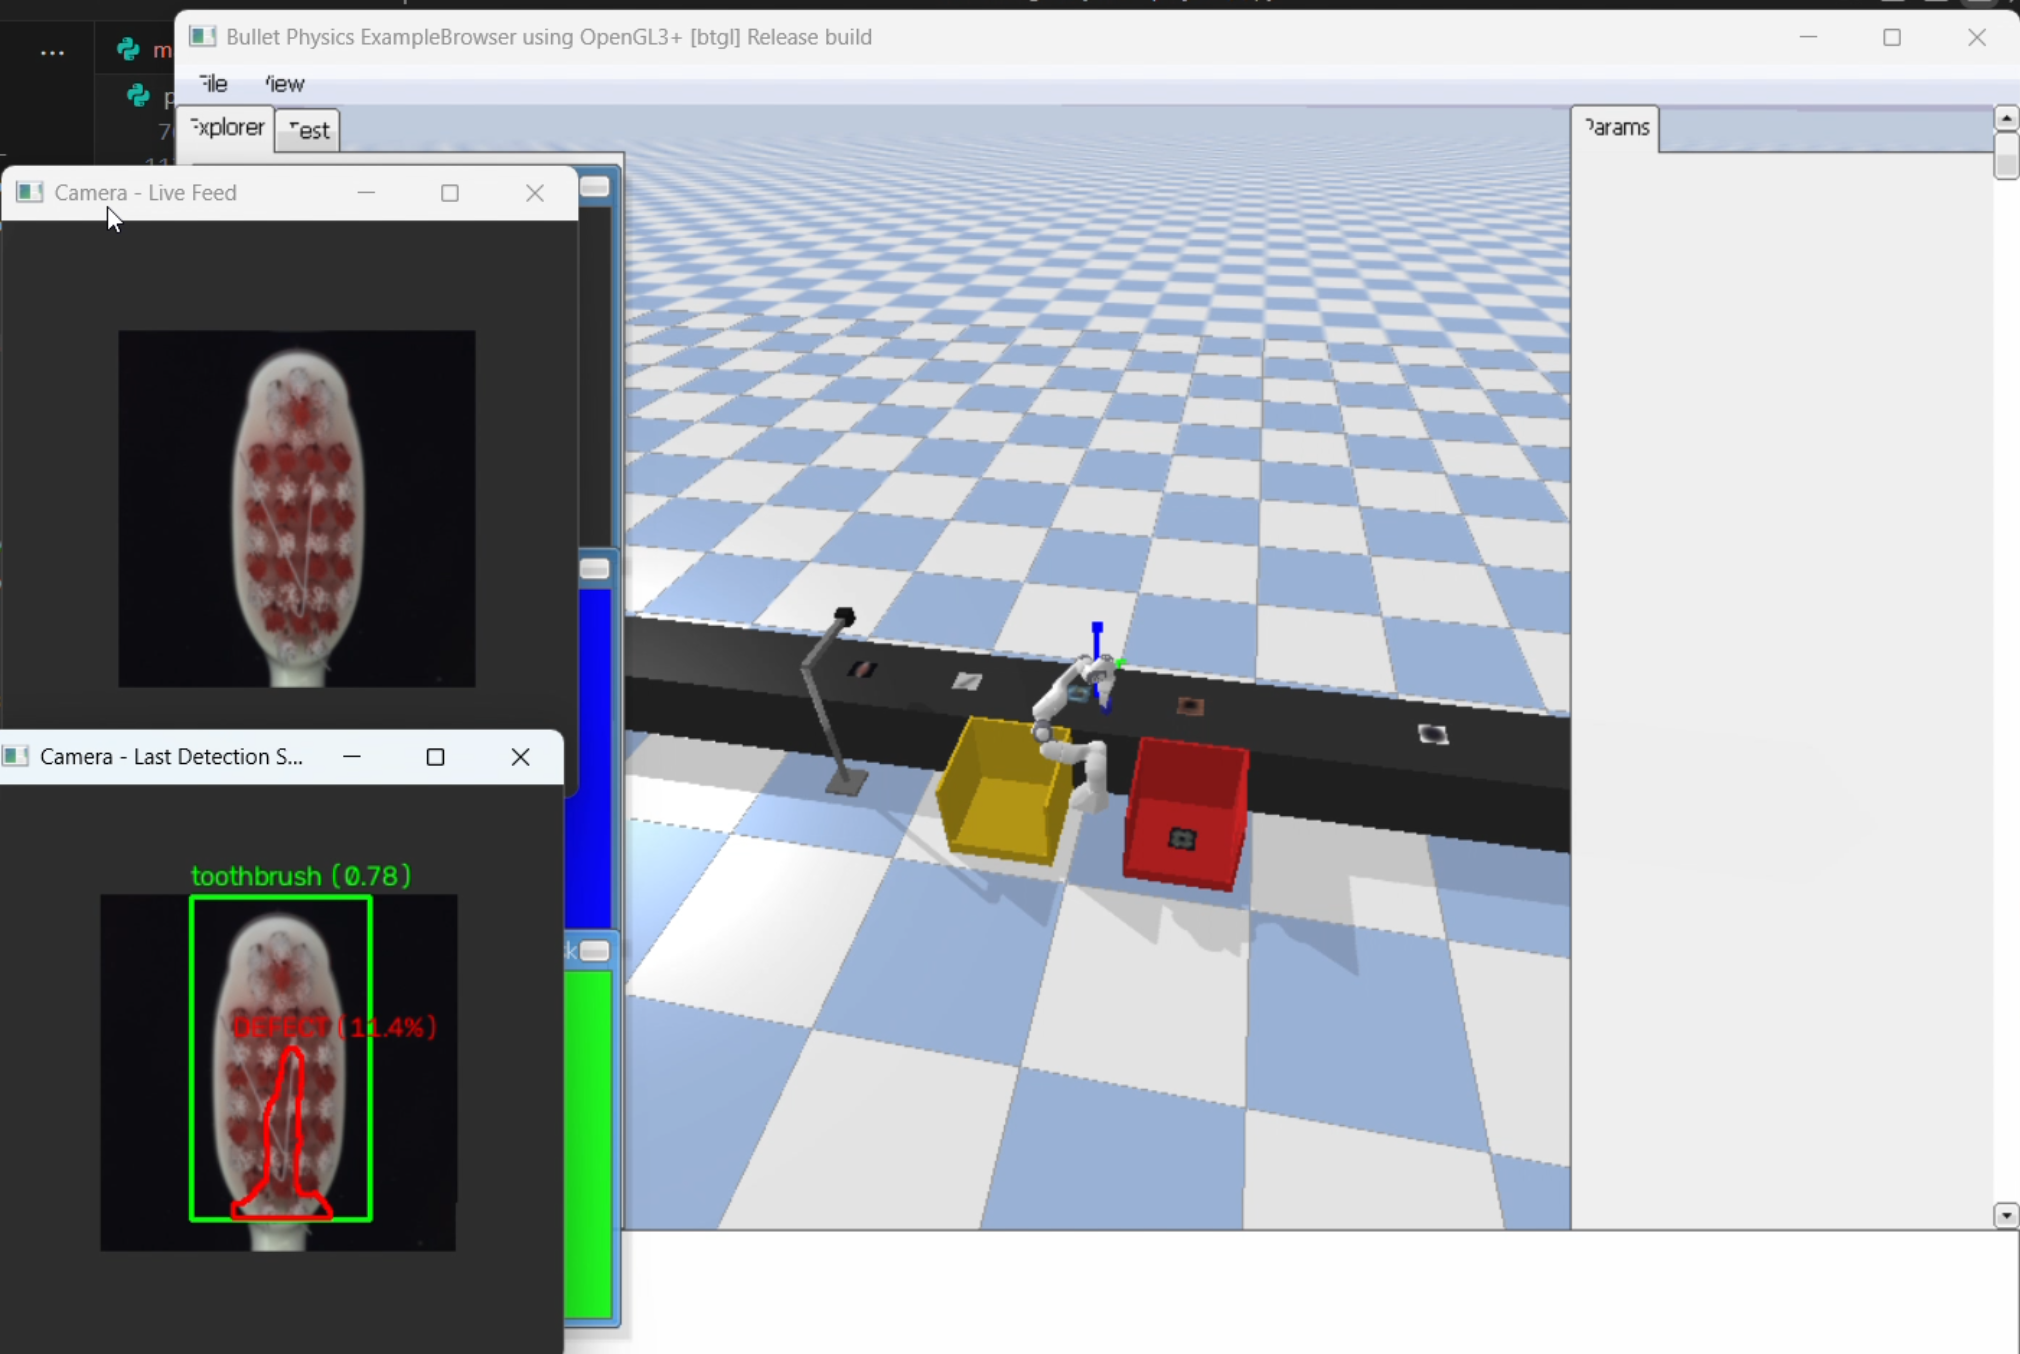
\includegraphics[width=0.85\textwidth]{img/fig32.png}
	\caption{Real-time defect segmentation and bounding box overlay interface.}
	\label{fig:fig32}
\end{figure}

\subsection{Execution Summary}
The execution run concluded with a graceful shutdown of active processing threads and a safe disconnect from the PyBullet server (\texttt{[SimManager] Disconnected from PyBullet}). The absence of blocking errors or frame rate drops during concurrent deep learning inference confirms the stability, memory efficiency, and real-time execution capabilities of the Digital Twin architecture.




\end{document}
